% Chapter 5

\chapter{Resolving Issues in the Beam Modulation Analysis}
\captionsetup{justification=justified,singlelinecheck=false}

\label{Ch:BMod_correction}

\lhead{Chapter 5. \emph{Resolving Issues}} 
A number of tests have been utilized to check the consistency and validity of the dithering analysis, focusing on three main questions. {\bf First}, is the analysis code working as expected and properly debugged? {\bf Second}, is the dithering solution self-consistent? It will be shown that a self-consistent analysis means: a) detector sensitivity to the modulation is removed and  b) the solution is independent of the selection of monitor or coil set used as long as both span the space of beam degrees of freedom. {\bf Third}, does the modulation solution reduce or remove correlations of the detectors to the beam monitors over long timescales?  

The first section of this chapter addresses each of these questions concerning the modulation analysis. Inconsistencies in the modulation analysis for Qweak are investigated and an attempt made to identify possible failure modes by looking at signatures of the failures. The last section of this chapter provides a method for dealing with the inconsistencies and assigning a systematic error. A  modulation correction and error is proposed for the subset of the full \Qs dataset for which valid modulation correction slopes were measured.

\section{Validating the Modulation Analysis}
The modulation analysis involves measuring detector and monitor responses to coils, using these to determine correction slopes $\frac{\partial D}{\partial M_k}$ and finally applying these correction slopes to the detector data. If this procedure is successful, the corrected data should be insensitive to the driving signal. An unsuccessful or partially successful correction will see a residual correlation to the driving signal, which in this case is a sinusoidal waveform. The detector (monitor) responses can be found by fitting a sinusoidal function to the detector (monitor) versus modulation phase data. The residual detector response is found by doing the same fit after the correction has been applied to the detector data. Figure \ref{fig:det_vs_ramp} shows an example of main detector bar 2 responses to the coils before and after correction. A small residual sine response can be seen on the upper left plot of response to Coil 0. These response plots are intended to clarify the discussion ahead.
\begin{figure}
\centering
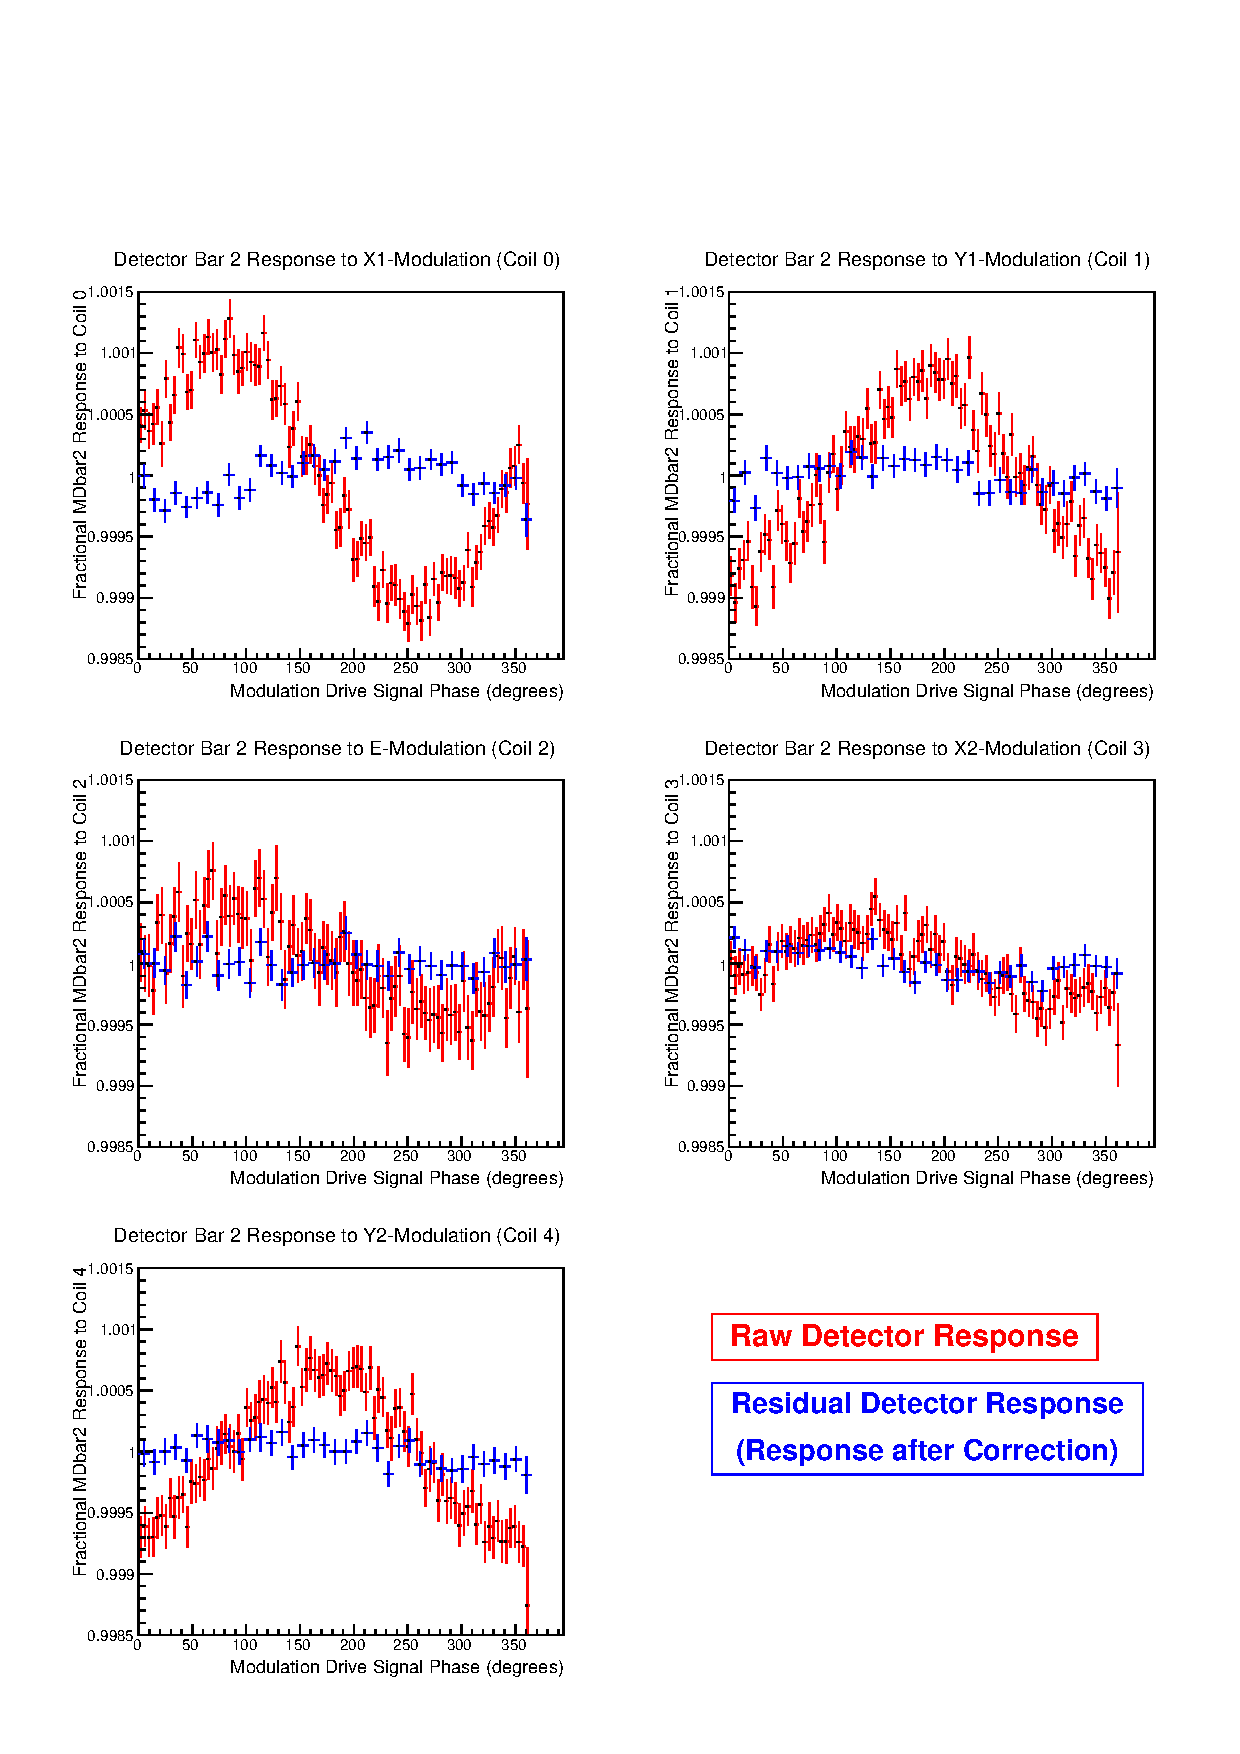
\includegraphics[width=5.8in]{./Pictures/MD_response_vs_coil.pdf}
\caption{\label{fig:det_vs_ramp}Normalized main detector bar 2 (chosen for its sensitivity to all modulation coils) responses to the five modulation coils shown versus drive signal phase. The responses before (red) and after (blue) correction are shown. A small residual response is evident in the plot of response to Coil 0 (upper left).}
\end{figure}

\subsection{Debugging the Analysis Procedure}

Early in the analysis, attempts to find a solution with 5 coils (sine-only) were only partially successful. One source of failure was found to be in the ``ramp'' variable used to keep track of the phase of the modulation drive signal. As previously mentioned, the ramp signal is just a saw-tooth signal sent to the DAQ in phase with and at the same frequency as the modulation signal. This saw-tooth signal was then pedestal subtracted and scaled such that its value was equal to the phase of the drive signal in degrees. A plot of ramp versus time can be seen in plot (a) of figure~\ref{fig:ramp_plots}. 
\begin{figure}[ht]

\centering
\framebox{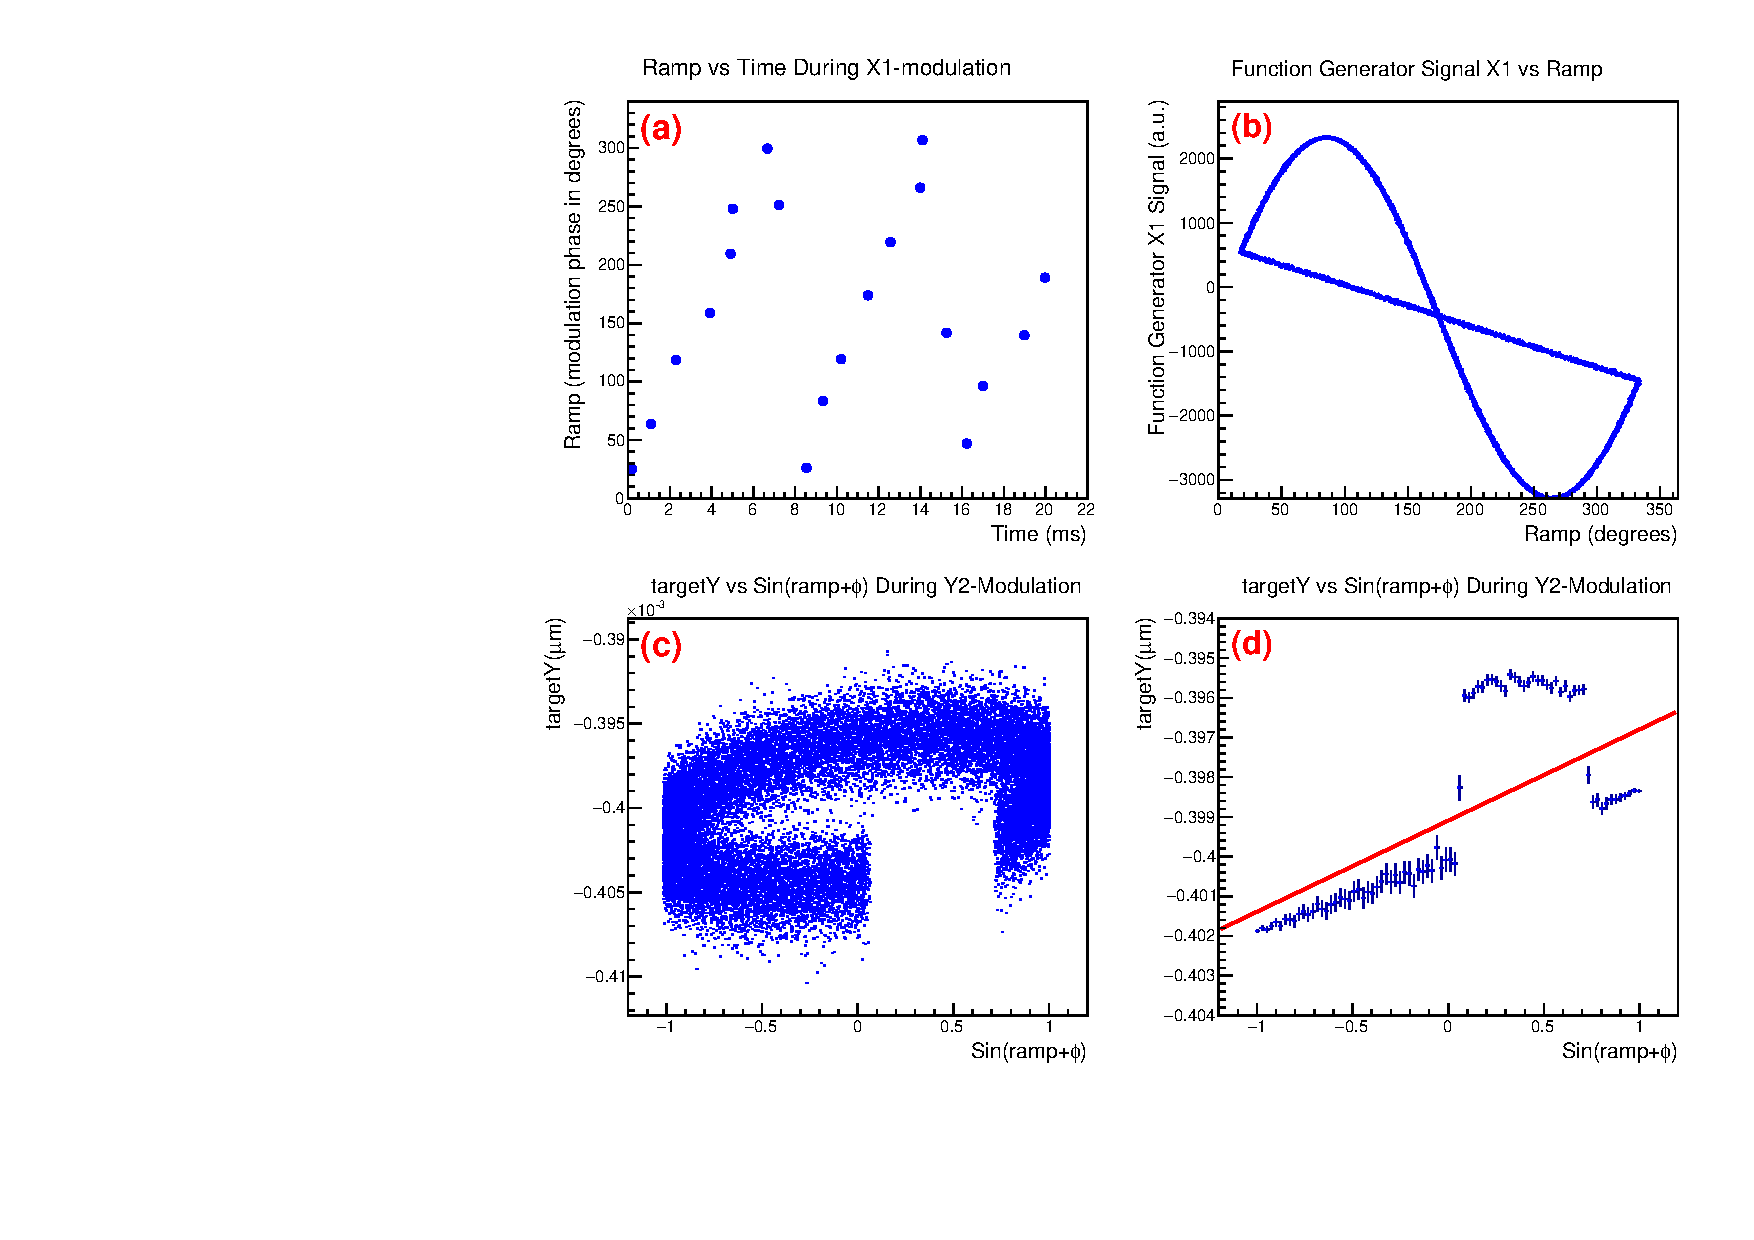
\includegraphics[width=5.5in]{Pictures/ramp.pdf}}
\caption{Various plots demonstrating ``ramp'' variable used to track modulation phase. (a). Ramp versus time showing the clear saw-tooth pattern. Signal integration ensures that phases near 0 and 360 are never reached. (b). Function generator signal driving the one of the horizontal modulation coils during X1 modulation plotted versus ramp variable. Signal integration improperly maps the return of the saw-tooth pattern making the line seen connecting 20 degrees and 340 degrees. (c). TargetY versus the sine of ramp plus and arbitrary phase offset. The combination of in and out-of-phase driving coils can produce elliptical responses in the monitors and detectors. When the improperly mapped phase in the saw-tooth return region is cut, a gap is left in the ellipse. (d). Profile plot (horizontal bin averages) of data from (c) with linear fit demonstrates how the coefficients of the sine and cosine responses can be biased by the missing region in ramp.}
\label{fig:ramp_plots}
\end{figure}
From the plot one can see that there are about 8 data points per cycle, consistent with a 125~Hz drive signal being sampled at 960~Hz. Because Qweak was an integrating experiment, the ramp signal was integrated over each MPS window (1~ms) of each sample, which ensured that points near 0 and 360 degrees could never be accessed. In fact, any ramp values which integrate over some portion of the fast return of the saw-tooth pattern will be incorrectly mapped to modulation phase. This can clearly be seen in plot (b) of  figure~\ref{fig:ramp_plots}. If one chooses to simply cut these incorrectly mapped events, a bias can be introduced into the sine and cosine response slopes found as seen in (c) and (d) of Figure \ref{fig:ramp_plots}. Early modulation results were subject to this bias until it was discovered and a simple solution implemented. A new variable ``ramp\_filled'' was created to replace ``ramp'' using a linear mapping from the ramp return region to the gap region of the ramp variable. Figure \ref{fig:ramp_filled} shows the same function generator signal seen in plot (b) of figure~\ref{fig:ramp_plots} but plotted against the new ``ramp\_filled'' variable.

\begin{figure}[ht]

\centering
\framebox{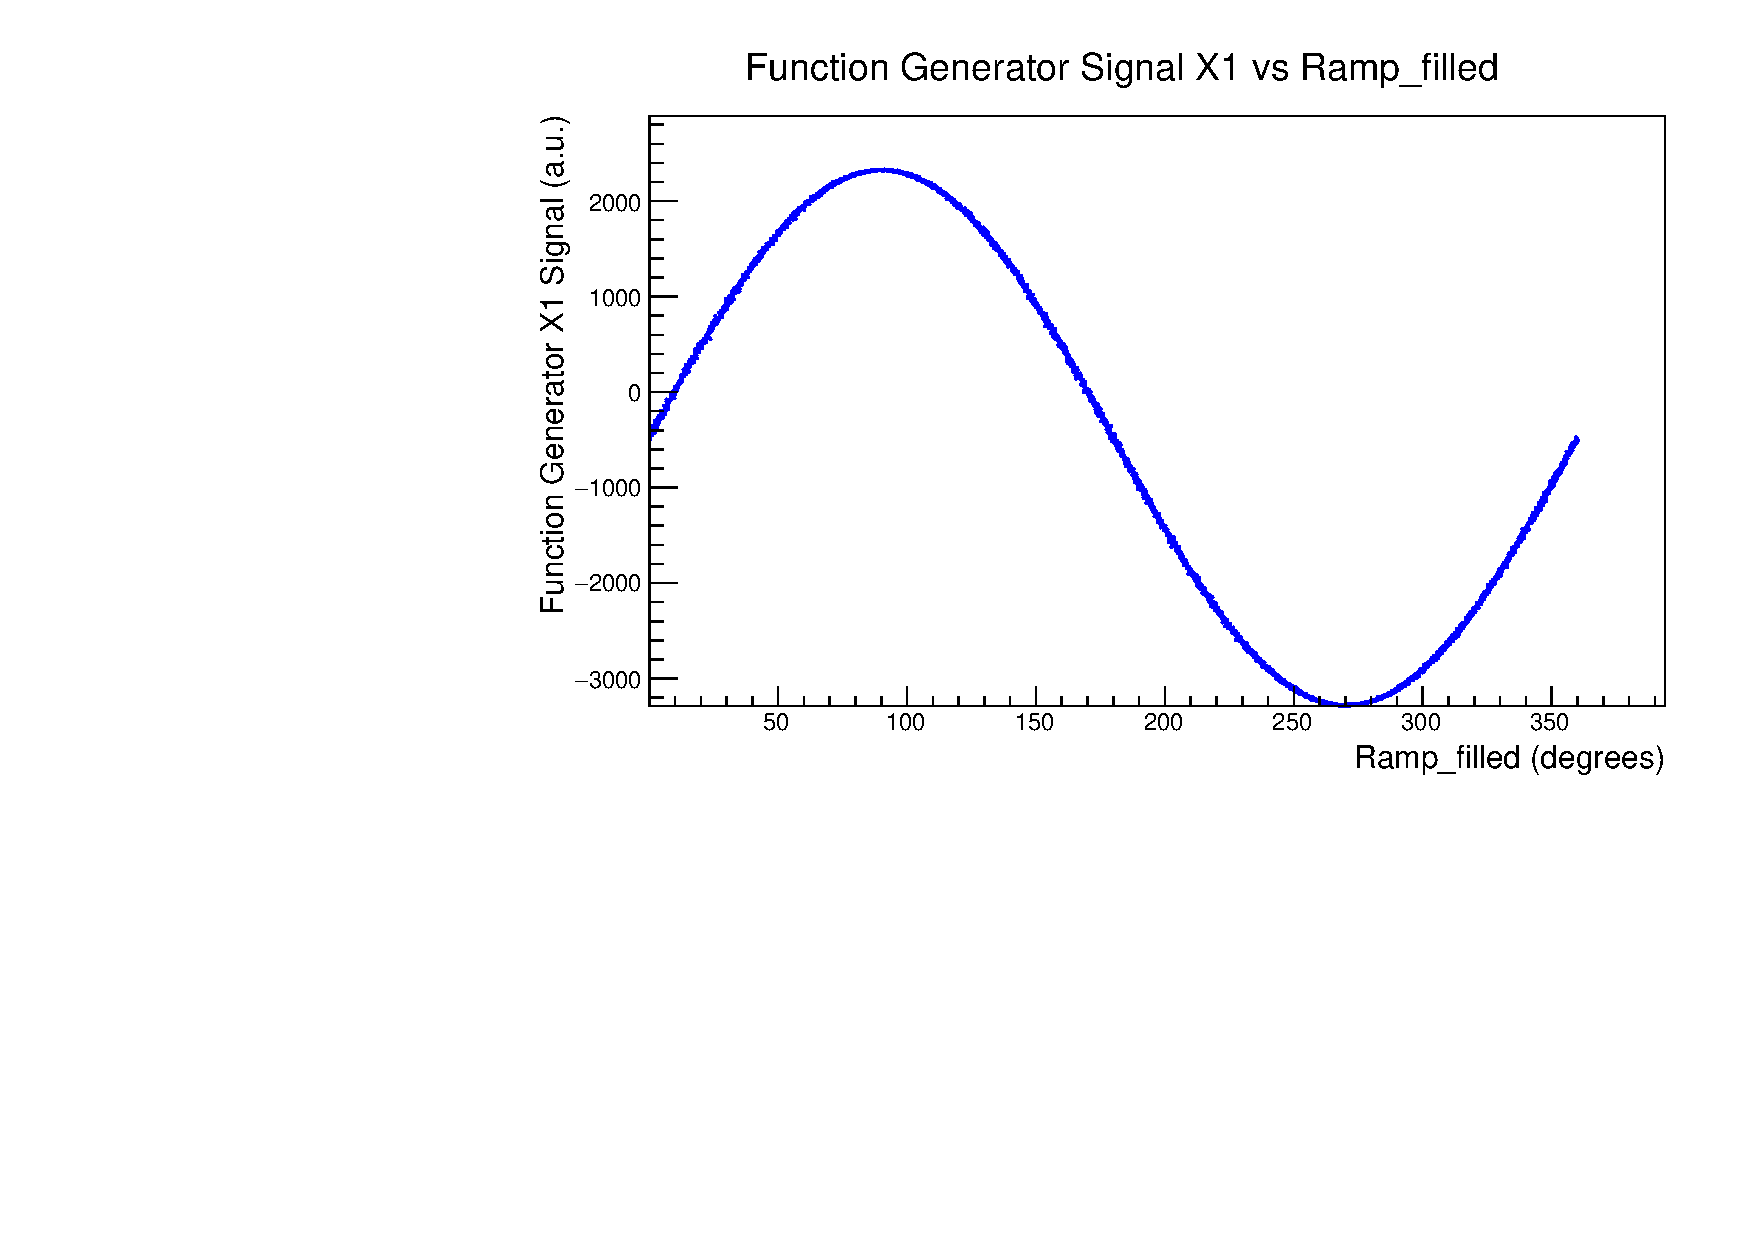
\includegraphics[width=3in]{Pictures/ramp_filled.pdf}}
\caption {Function generator X1 driving signal plotted versus ``ramp\_filled'' where the incorrect phases in ramp have been properly mapped back to ``fill'' the gap region.}
\label{fig:ramp_filled}
\end{figure}

An alternate solution to the problem of bias in the slopes from the gap region is to find both the sine and cosine coefficients simultaneously by fitting a function of
\[ 
\alpha+\alpha_{\sin}\sin(ramp)+\alpha_{\cos}\cos(ramp)
\]
to the detector and monitors versus ramp with the return region re-mapped or simply cut. An analytic solution to the coefficient values can be found making use of the known linearity of the monitor and detector response as follows:\\
\begin{equation*}\footnotesize
\left(\begin{array}{c}\sum_iQ_i\cos(\theta_i)\\\sum_iQ\sin(\theta_i)\\\sum_iQ\end{array}\right)=\left(\begin{array}{ccc}\sum_i\cos^2(\theta_i)&\sum_i\cos(\theta_i)\sin(\theta_i)&\sum_i\cos(\theta_i)\\\sum_i\sin(\theta_i)\cos(\theta_i)&\sum_i\sin^2(\theta_i)&\sum_i\sin(\theta_i)\\\sum_icos(\theta_i)&\sum_i\sin(\theta_i)&\sum_i1\end{array}\right)\left(\begin{array}{c}\alpha_{\cos}\\\alpha_{\sin}\\\alpha\end{array}\right),
\end{equation*}

with Q being the monitor or detector whose response is being measured and $\theta$ the modulation phase (ramp) and the sum going over the events in a given modulation cycle. In the final analysis, the exact analytic solution for the sine and cosine coefficients was utilized and the ``ramp\_filled'' variable was used to prevent unnecessary cutting of useful data. 

The function generator signals (see for example Figure \ref{fig:ramp_filled}) are expected to be proportional to the beam motion. Examples of detector responses to the drive signals were shown in Figure \ref{fig:det_vs_ramp}. A time history of the 5 raw sine response amplitudes for MDallbars is given in Figure \ref{fig:sine_only_res}. Also shown are the residual response amplitudes after correction using the 5-Coil sine-only analysis. The residual in-phase responses to modulation coils are indeed zero as required by linear algebra providing a first level cross-check of the analysis code.
\begin{figure}[h]

\centering
\framebox{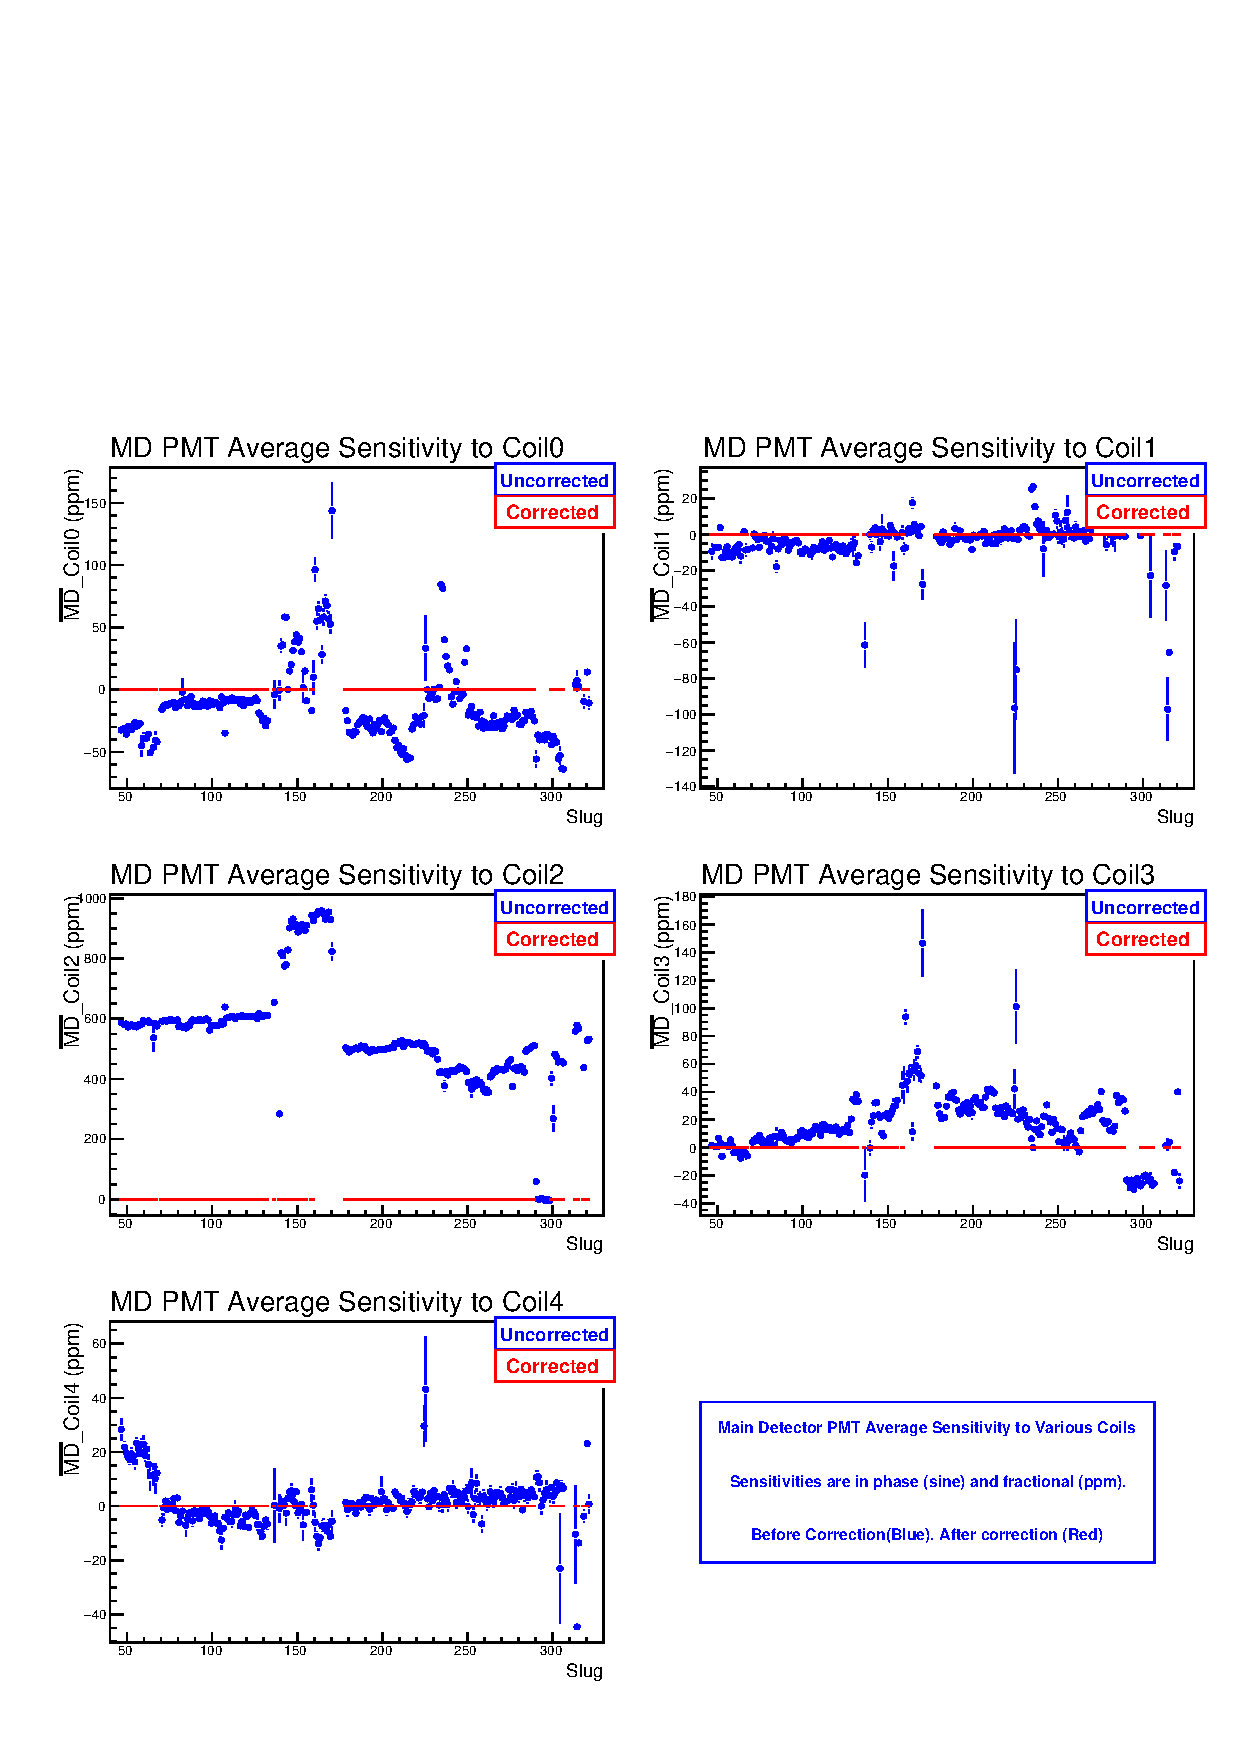
\includegraphics[width=5.5in]{Pictures/sine_only_residuals.pdf}}
\caption{Main detector average in-phase (sine) response to the five different types of modulation. Blue is the raw responses and red is the residual response after the modulation corrections have been applied. Only the in-phase (sine) responses of detectors and monitors have been used in this analysis, so the residuals must be 0 by definition if the analysis code is working properly.}
\label{fig:sine_only_res}
\end{figure}


\subsection{\label{sctn:inconsistency}Inconsistency Arising from Redundancy}
As previously mentioned, the subject of inconsistency in the modulation analysis naturally lends itself to two divisions:\\ 1). Inconsistency in the over-determined equation set manifesting itself as a residual sensitivity to modulation after correction.\\
2). Inconsistency in total correction to the dataset prescribed by parallel analyses using different coil selections.\\ Although these are related and it would appear that the first leads directly to the second, we will see that it is possible in some instances to have analyses whose differences in prescribed corrections cancel over time to produce a consistent net correction. The following two subsections individually deal with each of these two types of inconsistencies in the dataset. 
\subsubsection{Residual Sensitivity to Modulation}
While introducing extra coils provides a way of reducing the uncertainty in the solution, it also provides a way of recognizing potential inconsistencies in the set of linear equations used.  Residual sensitivity of detectors to modulation after correction is the first place to look for this inconsistency. Figure \ref{fig:10coil_and_sine_only_res} compares the residual sensitivity of MDallbars to the modulation coils for a sine-only analysis and a 10 coil analysis. If one only had access to the 5 coils of the sine-only analysis, that is, if FFB were paused during modulation and only 5 modulation patterns were used, the inconsistency in the modulation system/analysis would be hidden. The residuals would not be a useful criterion for determining the effectiveness of the applied correction. With more than 5 coils, the total residual is minimized but not forced to be zero like the solution shown in figure~\ref{fig:sine_only_res}. Equation~\ref{eq:chisquaresolution_no_variance} shows that the ``total residual'' being minimized is given by
\begin{equation}
Total~Residual=\sqrt{\sum_{i=1}^{N}\left(\frac{\partial D_d}{\partial C_i} - \sum_{m=1}^{5}\frac{\partial D_d}{\partial M_m}\frac{\partial M_m}{\partial C_i} \right)^2}.
\label{eq:total_residual}
\end{equation}

For the \Qs modulation dataset, analyses with different complete coil sets yield systematically different solutions, pointing to a problem in either the data or the analysis procedure. With 10 coils (probably only 9 useful ones) available, there are dozens of sets of independent coils that adequately span the phase space, and while the author has not analyzed all of the possible sets, the 32 schemes he has completed present a not-so-consistent picture. Figure~\ref{fig:chisquare_vs_slug} compares the total residuals for a few different coil selections and clearly illustrates that the 10 coil analysis always produces the minimum total residual as defined by equation~\ref{eq:total_residual}.
\begin{figure}[t]

\centering
\framebox{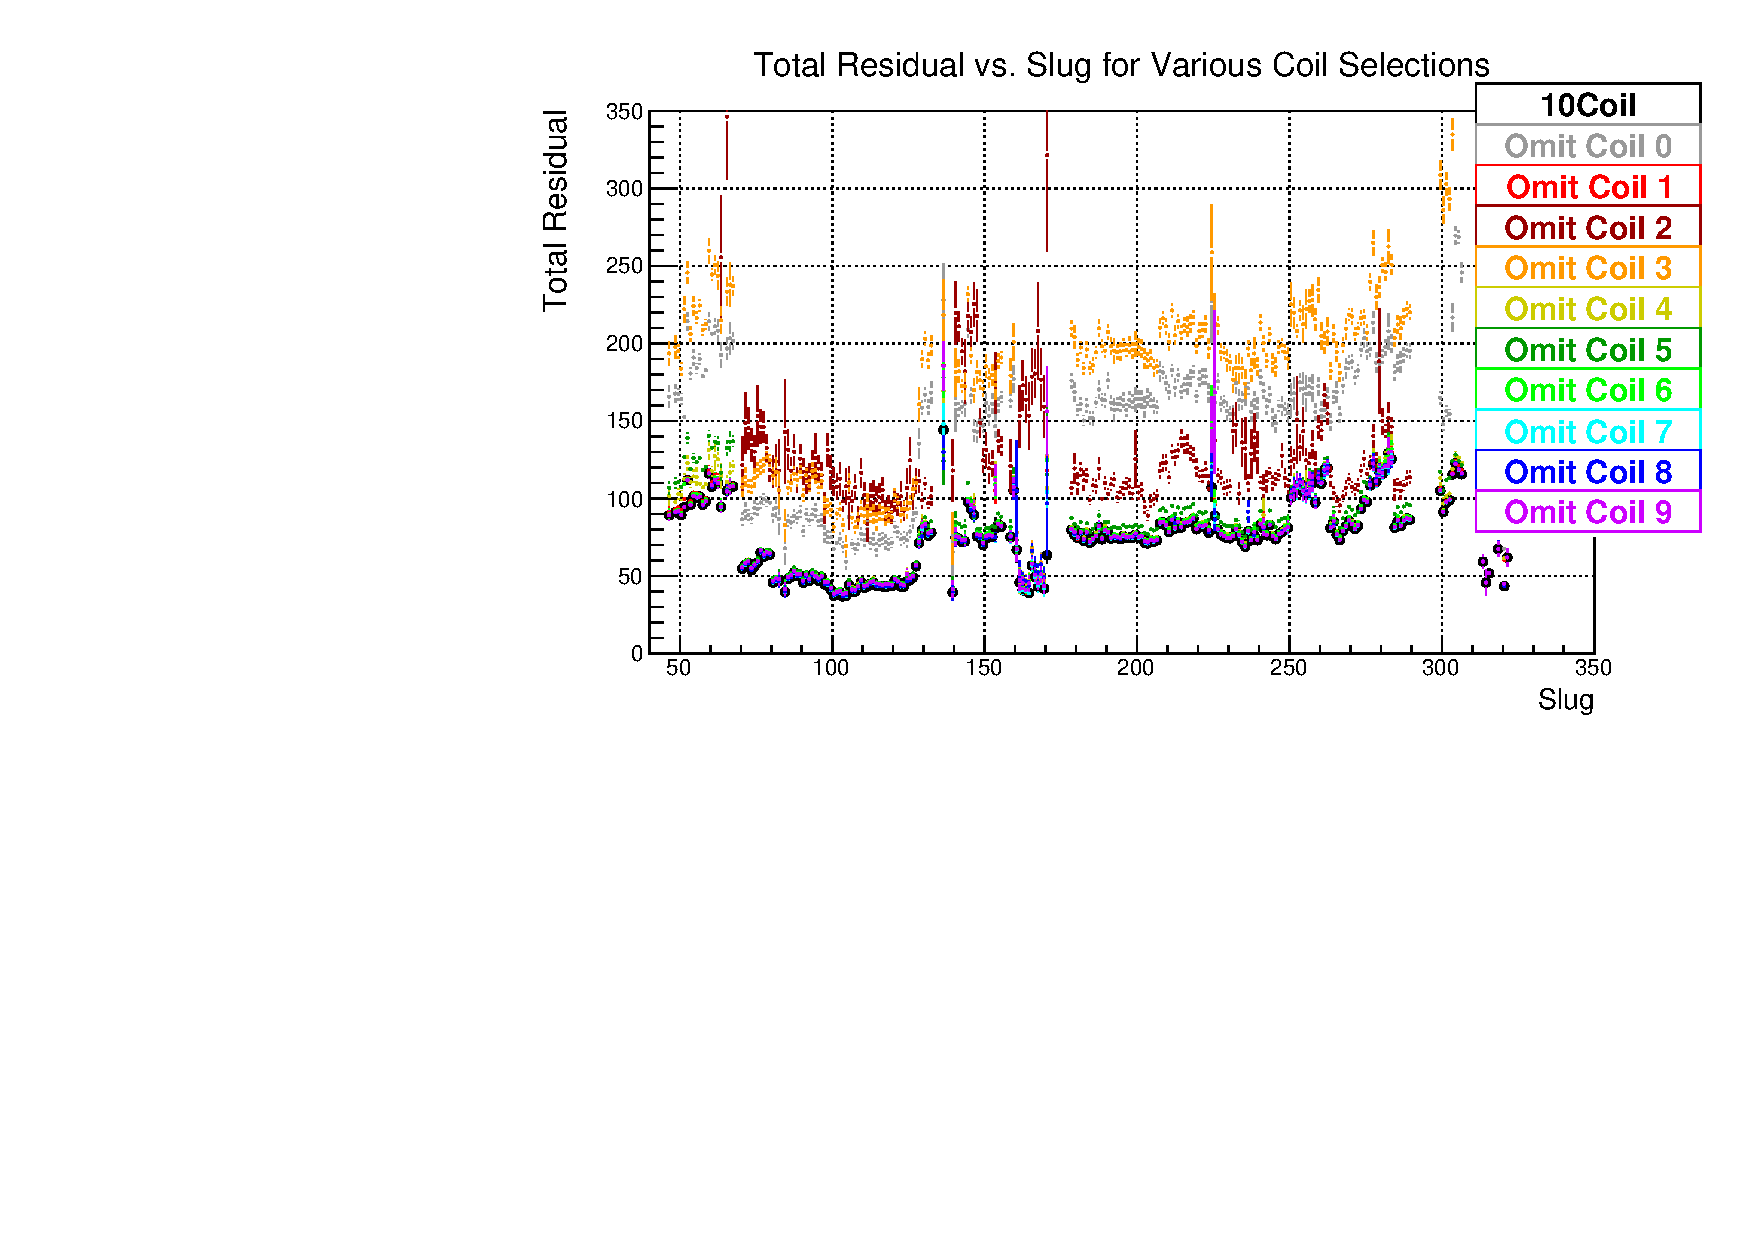
\includegraphics[width=5in]{Pictures/ChiSquare_vs_slug.pdf}}
\caption{Comparison of total residual (Equation \ref{eq:total_residual}) versus slug for analyses with various coil selections.}
\label{fig:chisquare_vs_slug}
\end{figure}

If the residuals are a result of a problem in the analysis procedure, then the analysis should also fail to correct beam position monitors, that is, it should fail to remove monitor sensitivity to the modulation coils just as it fails in the detector correction. In a linear optics model for the electron beam a complete set of beam position monitors that are sufficiently sensitive to the phase space of beam position, slope and energy should be able to predict the response of any other monitor. Of course, given the modulation calibration procedure for determining monitor responses, a prediction will only be available for monitors downstream of the modulation coils. In principle, therefore, a complete\footnote{In this context ``complete'' means that you have a set of monitors that spans the 5 dimensional space of position, slope and energy''} set of 5 monitors should provide sufficient information to predict any other monitor and with properly measured correction slopes be able to completely remove sensitivity to modulation. 

\begin{sidewaysfigure}[t]

\centering
\framebox{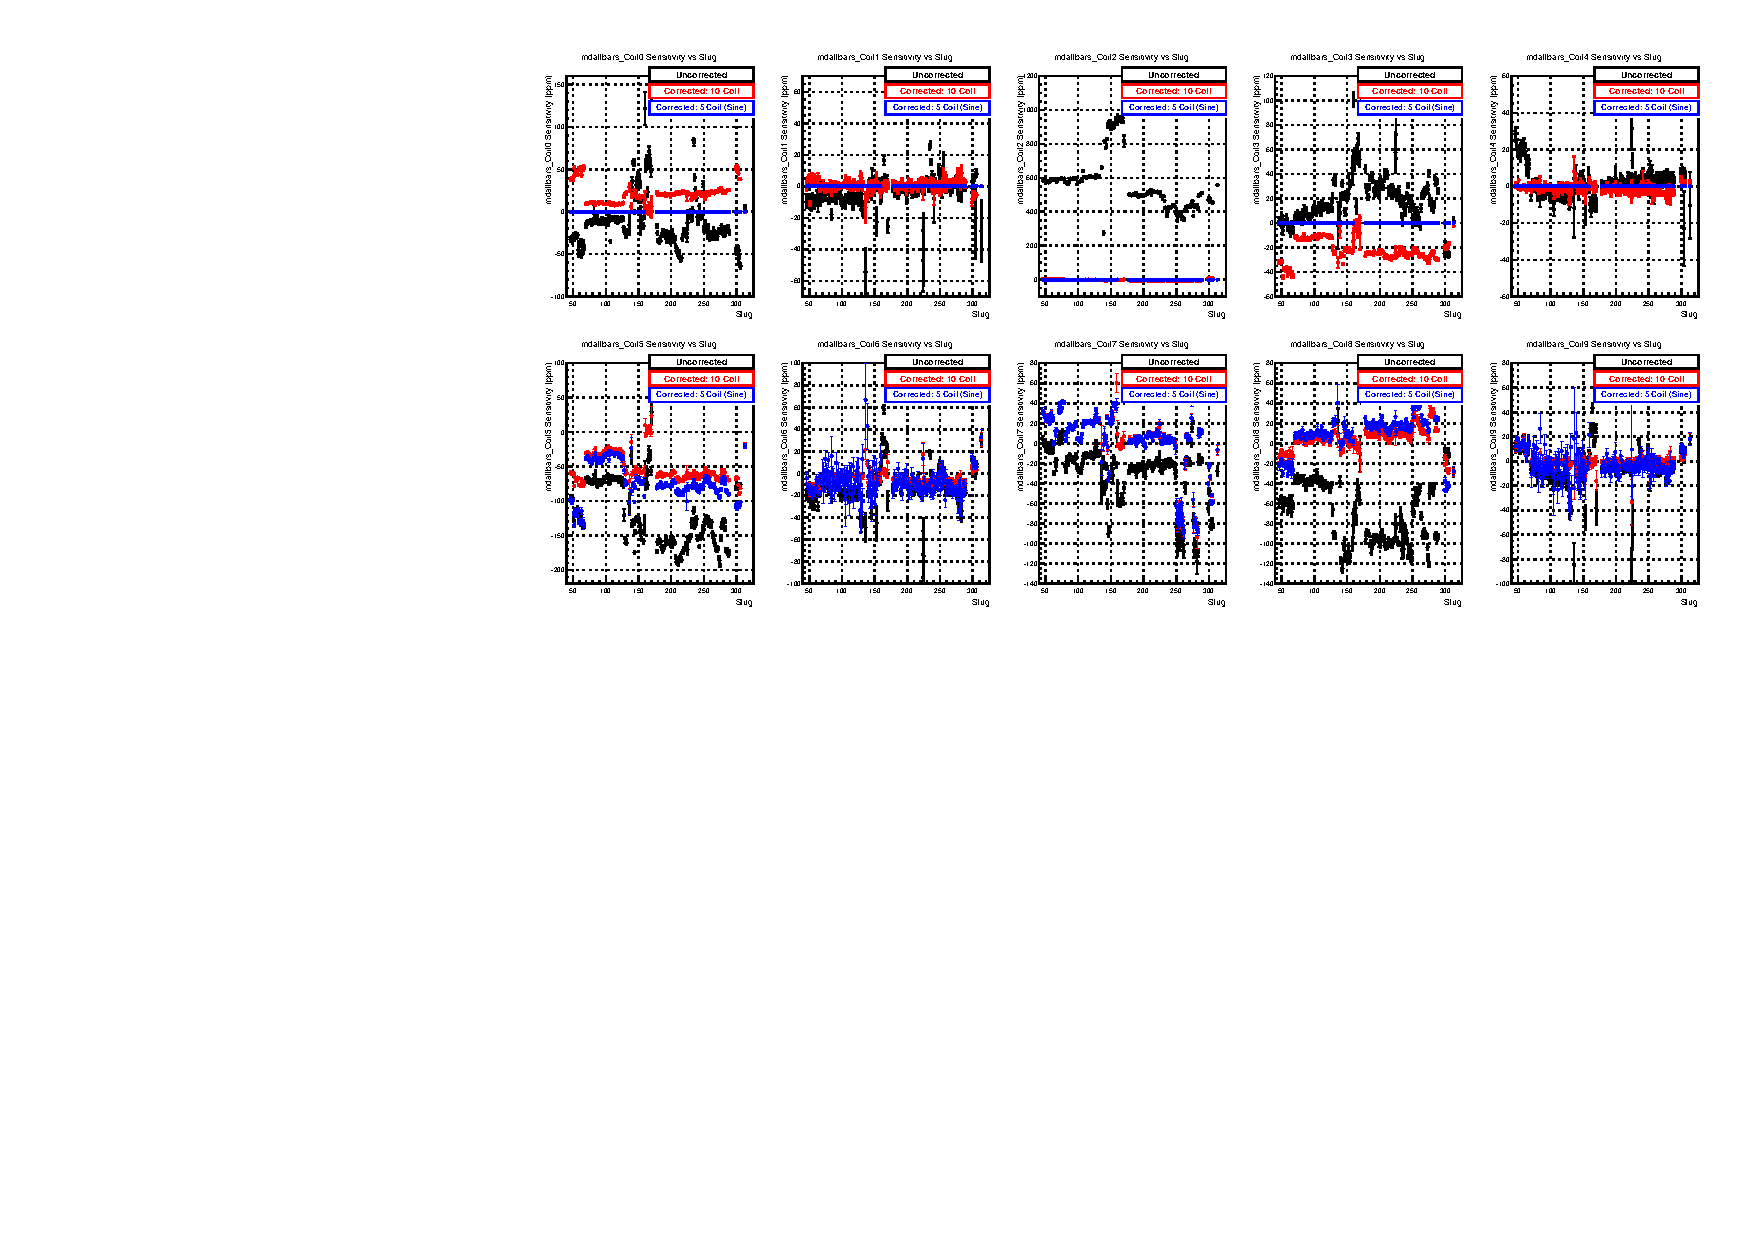
\includegraphics[width=8.9in]{Pictures/Residuals10CoilandSineOnly.pdf}}
\caption{Comparison of residual MDallbars responses to the five different types of modulation. Black is the raw uncorrected responses and red is the residual response after correction using a 10-Coil analysis  and blue is the residual response after the 5-Coil (sine-only) modulation corrections have been applied. The 10-Coil analysis by definition gives the smallest collective least squares residual. Each plot represents a single term in the summation in equation~\ref{eq:total_residual}. It becomes apparent that the sine-only analysis creates a 0 in-phase residual response by increasing the residual out-of-phase response.}
\label{fig:10coil_and_sine_only_res}
\end{sidewaysfigure}

\begin{sidewaysfigure}[t]

\centering
\framebox{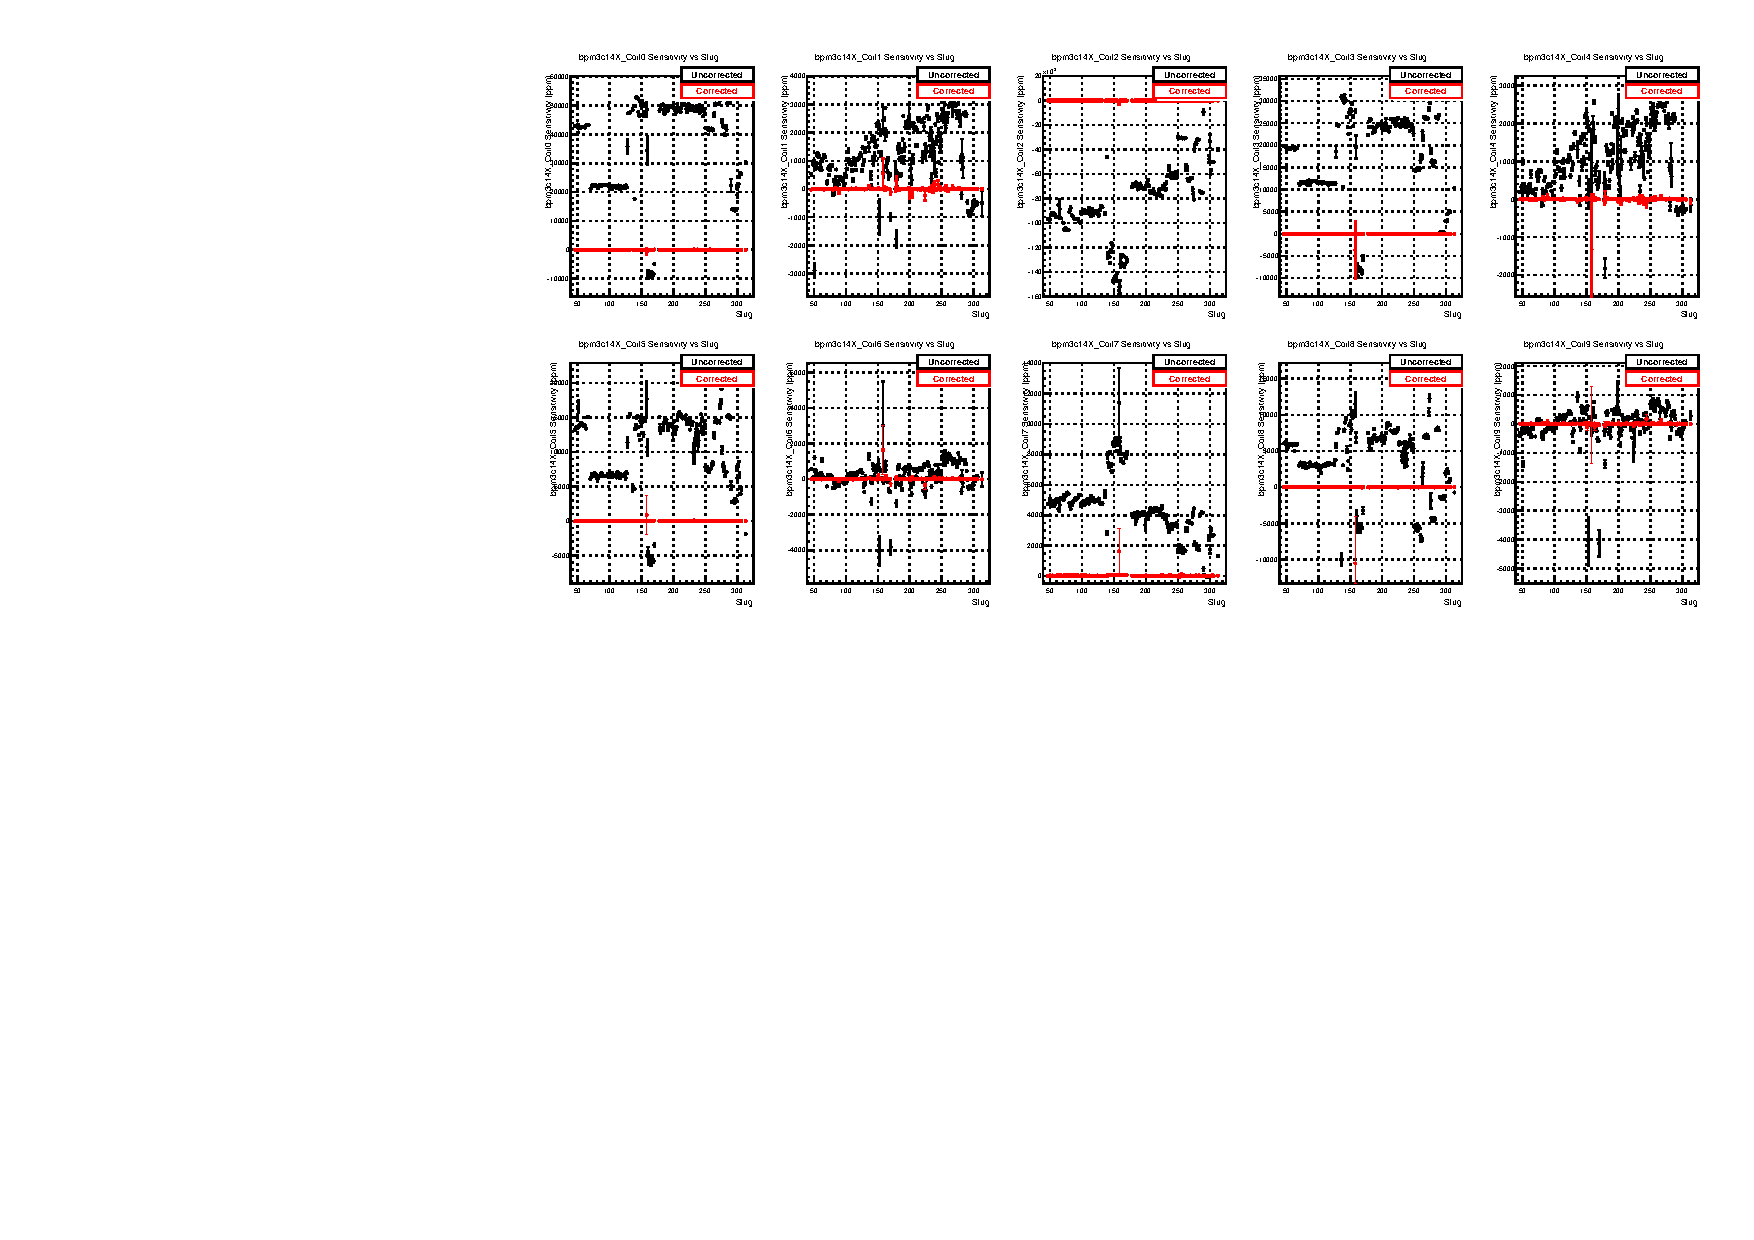
\includegraphics[width=8.9in]{Pictures/Residual_bpm3c14X.pdf}}
\caption{Comparison of residual bpm3c14X responses to the five different types of modulation. Black is the raw uncorrected responses and red is the residual response after correction using a 10-Coil analysis. The sensitivity to the modulation coils is almost completely removed by the correction using targetX, targetXSlope, targetY, targetYSlope, and bpm3c12X.}
\label{fig:residual_bpm3c14X}
\end{sidewaysfigure}
\begin{sidewaysfigure}[t]

\centering
\framebox{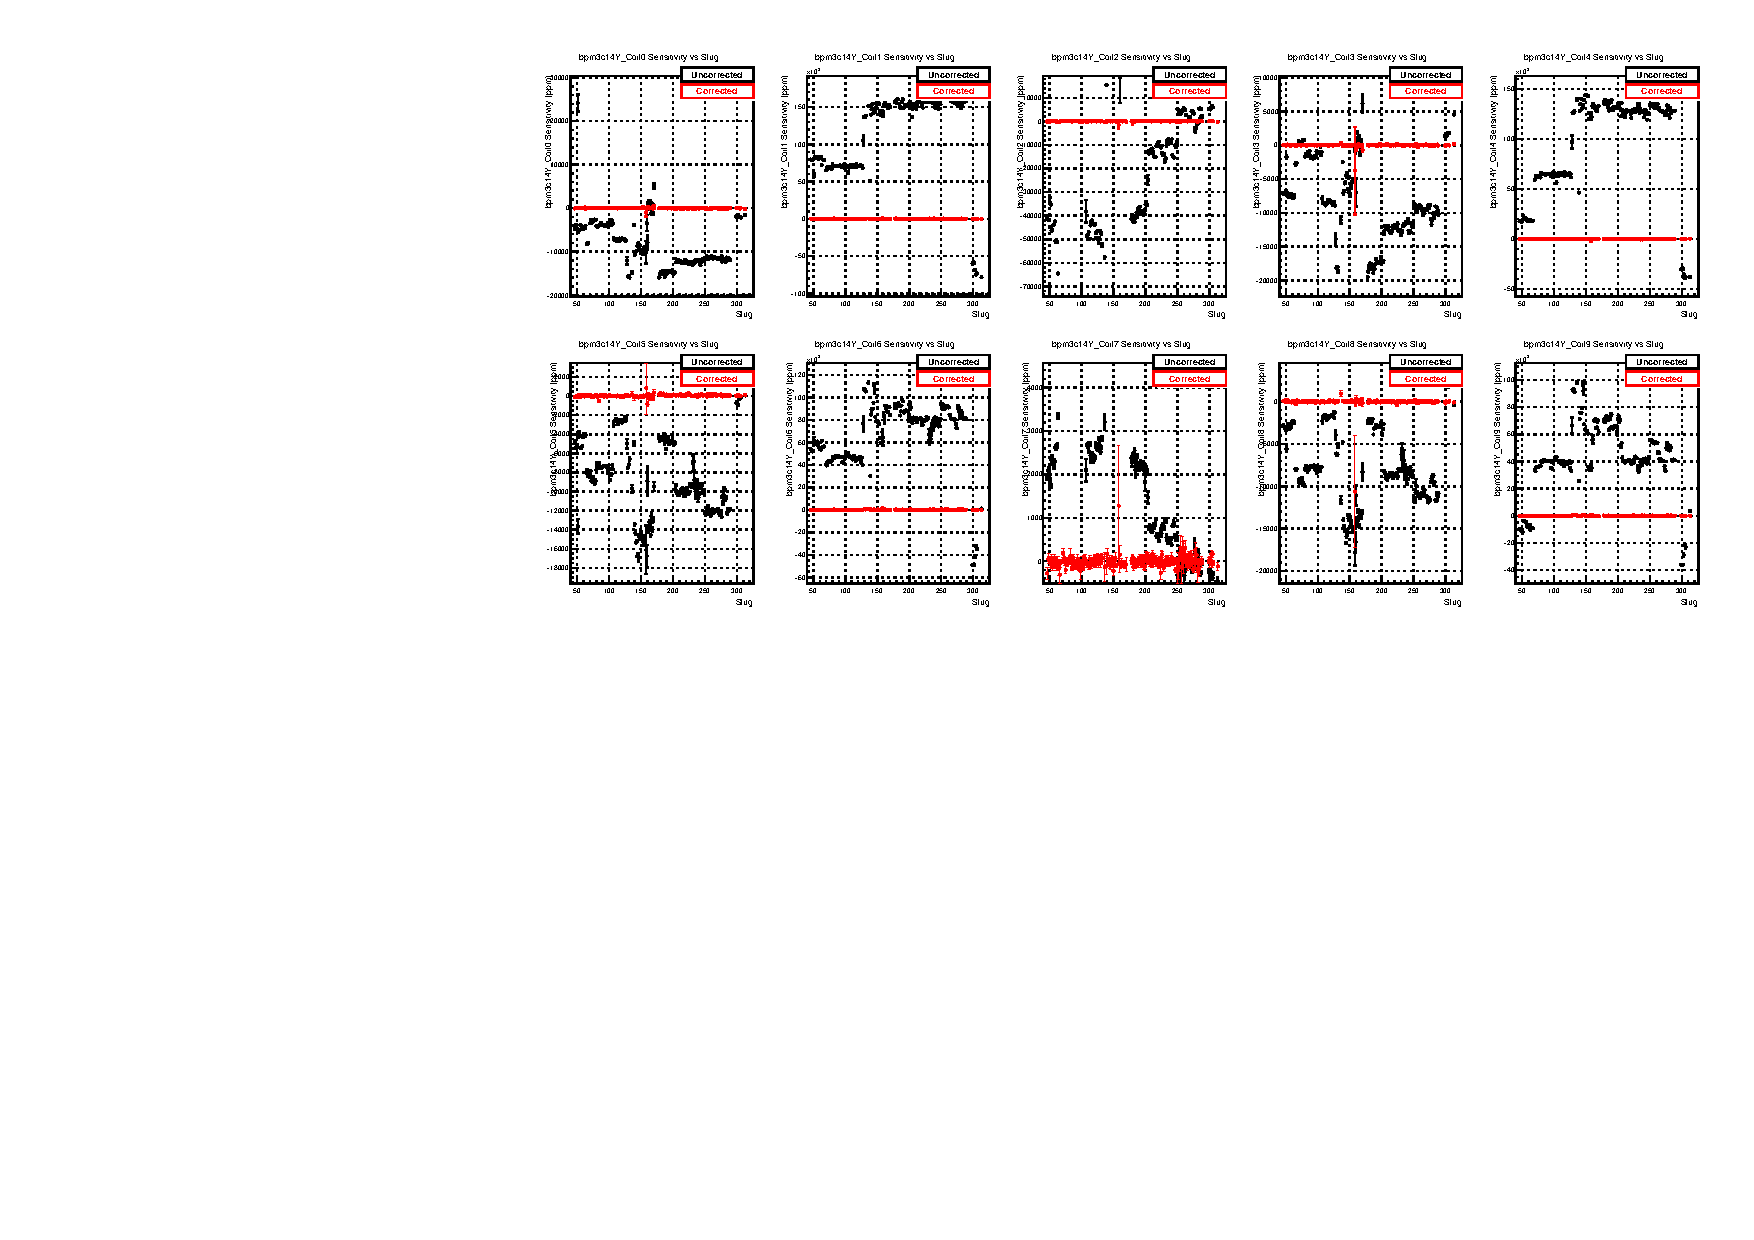
\includegraphics[width=8.9in]{Pictures/Residual_bpm3c14Y.pdf}}
\caption{Comparison of residual bpm3c14Y responses to the five different types of modulation. Black is the raw uncorrected responses and red is the residual response after correction using a 10-Coil analysis. The sensitivity to the modulation coils is almost completely removed by the correction using targetX, targetXSlope, targetY, targetYSlope, and bpm3c12X.}
\label{fig:residual_bpm3c14Y}
\end{sidewaysfigure}

A set of monitors not included in the 5 used for the correction were treated as detectors in the analysis code and corrected to remove sensitivity to modulation. The analysis showed that the monitors chosen for the correction (4 target variables plus bpm3c12X) are effective at correcting other monitors. Thus, once the responses of the electron beam to position, angle and energy changes at a given location along the beamline have been calibrated to the responses of the five monitors to the same changes, then any given response at that location can be accurately predicted using only the five monitors. The modulation analysis is simply an accurate calibration procedure. Figures \ref{fig:residual_bpm3c14X} and \ref{fig:residual_bpm3c14Y} compare the uncorrected and corrected sensitivities of the beam position monitor at girder 3c14 on the Hall C beamline. The horizontal beam response is given by bpm3c14X and vertical response by bpm3c14Y. Notice how well the monitor response is zeroed after correction when compared with the MDallbars response in figure~\ref{fig:chisquare_vs_slug}. 
\FloatBarrier
A number of conclusions can be drawn from the study where monitors are corrected to remove modulation sensitivity:
\begin{itemize}
\item{This provides a second validation of the analysis procedure and code (the first being the residuals going to 0 with equal number of monitors and coils.)}
\item{The expected 5 degrees of freedom seem sufficient to describe the responses of the monitors.}
\item{Any model for the main detector residuals involving a failure of the monitors must specifically be able to explain their success in correcting other monitors. This observation narrows the space of allowed failure models.}
\item{It appears that the detectors are sensitive to some effect that the monitors do not measure, at least not well. This effect may be a real beam property like halo or spot size that the monitors do not resolve well. Alternately, it could be an artifact introduced to the detectors by the coils themselves such as noise or pedestal shifts coherent with the modulation signal.}
\end{itemize} 
Although equation~\ref{eq:total_residual} guarantees the 10-Coil analysis will provide the smallest total residual, it is not guaranteed to provide the optimal correction slopes. Furthermore, if one chooses to calculate the residual differently by only summing over a subset of the coils, the 10-Coil solution will not always be optimal in terms of residual size. Figure~\ref{fig:residual_omit38} demonstrates that when the residuals arising from coils 3 and 8 are omitted from the summation (see Table \ref{tab:coil_nomenclature} for definition of coils), the 10-Coil analysis yields a much larger residual than does the analysis where the same coils are omitted in the slope calculation. The residual shown is given as
\[
Residual=\sqrt{\sum\limits_{\substack{i=1\\i\neq 3,8}}^{10}\left(\frac{\partial D_d}{\partial C_i} - \sum_{m=1}^{5}\frac{\partial D_d}{\partial M_m}\frac{\partial M_m}{\partial C_i} \right)^2}.
\]
\begin{figure}[h]

\centering
\framebox{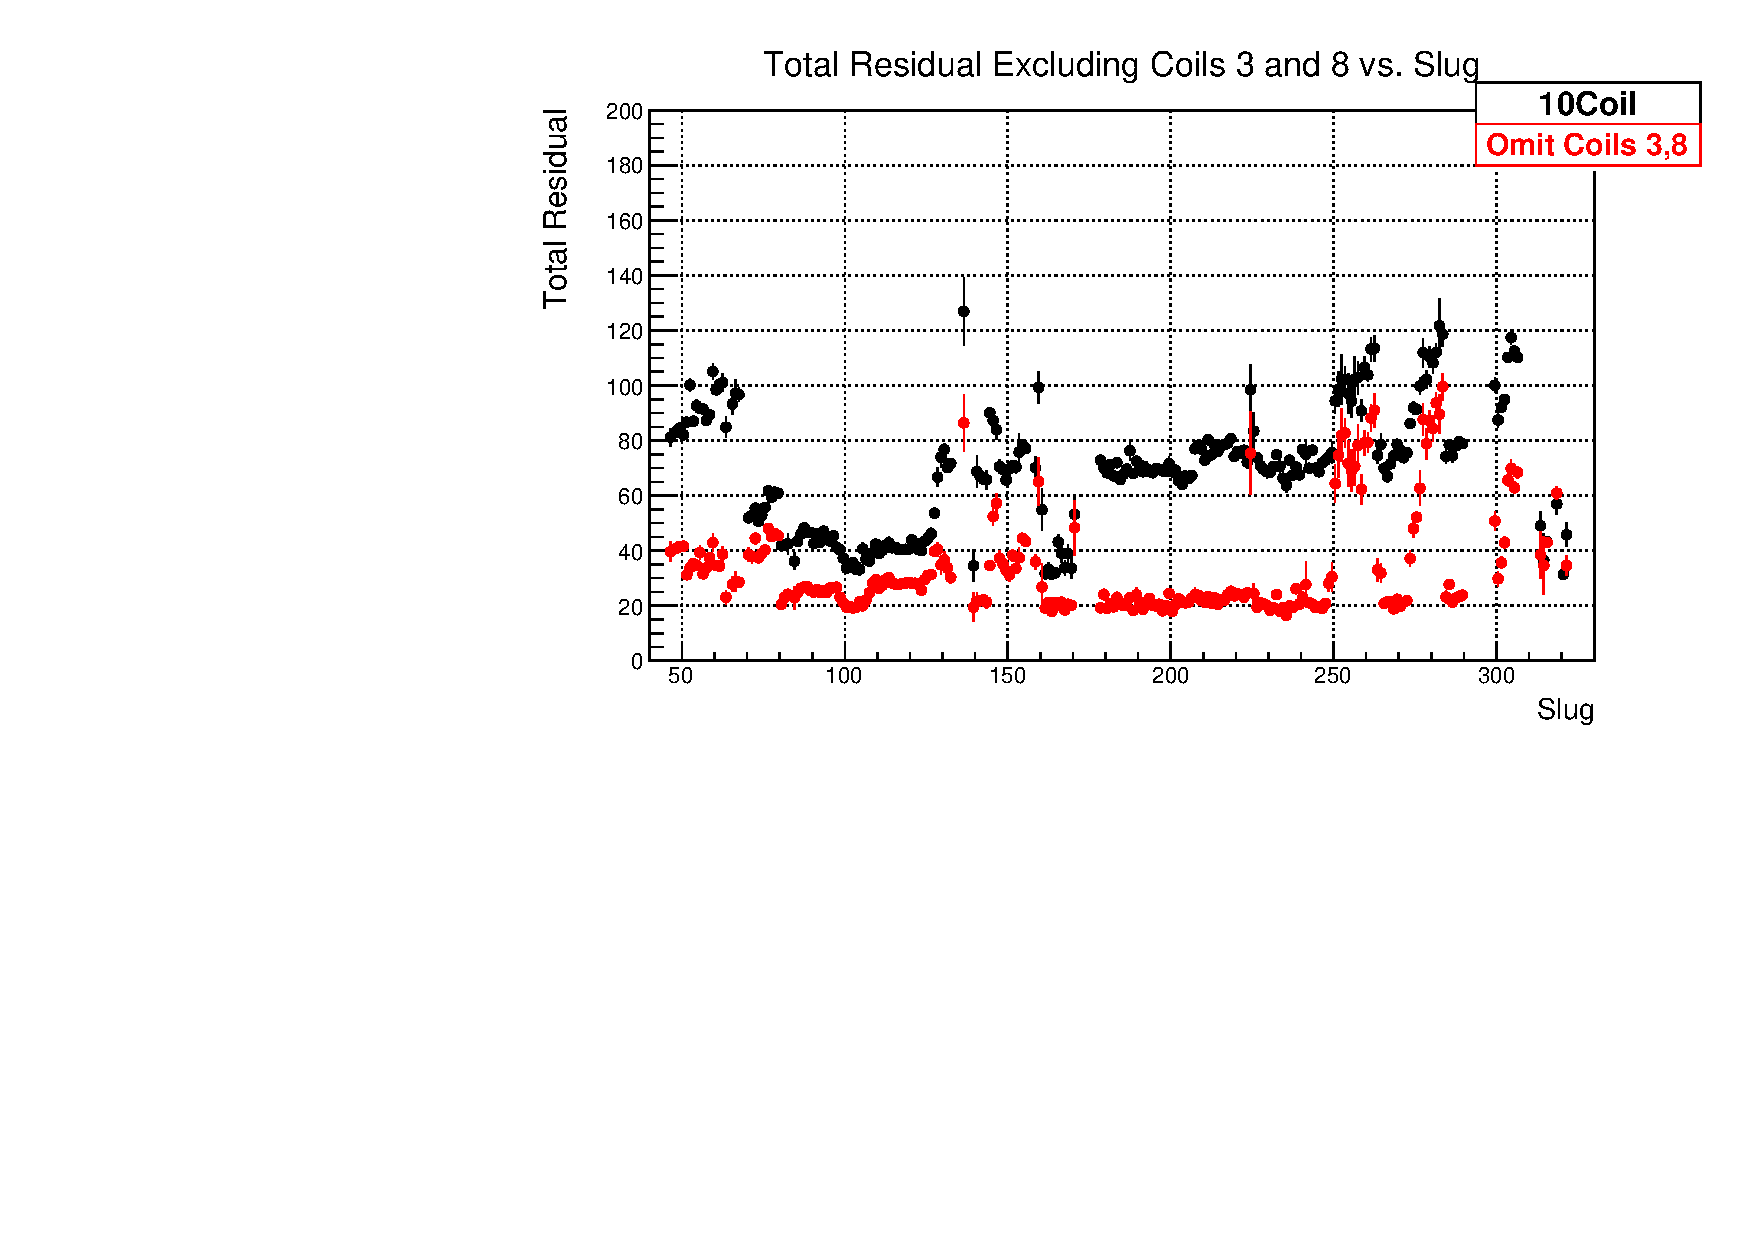
\includegraphics[width=3.5in]{Pictures/ChiSquare_vs_slug_omit38.pdf}}
\caption{Comparison of total residual responses after correction using slopes from a 10-Coil analysis and those from an 8-Coil analysis where coils 3 and 8 are omitted. In this plot, the residual is calculated omitting the residuals from coils 3 and 8 as well. Coils 3 and 8 are associated with X2-modulation. If an issue were found with the X2-modulation coils, for example, this particular residual calculation would be of more interest than the full residual over 10 coils.}
\label{fig:residual_omit38}
\end{figure}


\begin{table}[!h]
\caption{Modulation coil nomenclature used in the analysis discussion.}
\begin{center}
\begin{tabular}[h]{|c||c|c|}\hline
Modulation&In-Phase Response&Out-of-Phase Response\\
Type&(Sine Amplitude)&(Cosine Amplitude)\\\hline\hline
X1-Type&Coil 0&Coil 5\\
X2-Type&Coil 3&Coil 8\\\hline\hline
Y1-Type&Coil 1&Coil 6\\
Y2-Type&Coil 4&Coil 9\\\hline\hline
E-Type&Coil 2&Coil 7\\\hline
\end{tabular}
\end{center}
\label{tab:coil_nomenclature}
\end{table}

One could imagine situations where cumulative evidence might force one away from the default 10-Coil choice.  Imagine, for example, a situation where it was found that whenever a particular modulation coil was active, an artifact appeared in the data that was inconsistent with what is known to be true about the system. One such example investigated was the introduction of noise coherent with the drive signal into the detector data. If a response to the modulation signal in any modulation period were found in a channel known to have no correlation with beam dynamics, this would signal a problem with electronics pickup possibly biasing the results. In that case, it would be wise to remove any coils associated with this artifact from the calculation of both the correction slopes and the residuals. 

One detector channel in the \Qs analysis chain was fed by a signal from a battery and was setup to test for effects such as the one mentioned in the previous paragraph. Any response to modulation seen on this channel would certainly be a sign of electronics pickup. Although the data for this channel was not analyzed over the whole \Qs dataset, the response for a randomly chosen period was found to be nearly consistent with zero. Figures \ref{fig:isourc} and \ref{fig:cagesr} show the response of the null channels ``qwk\_isourc'' and ``qwk\_cagesr'' for a period near the beginning of Run 1 (between runs 10000 and 10200). Comparison of the responses of the null channels to the main detector response shows that they are typically 3 orders of magnitude apart, which is far too small an effect to account for the highly non-zero MDallbars residual response at the beginning of Run 1.
\begin{figure}[ht]
\centering
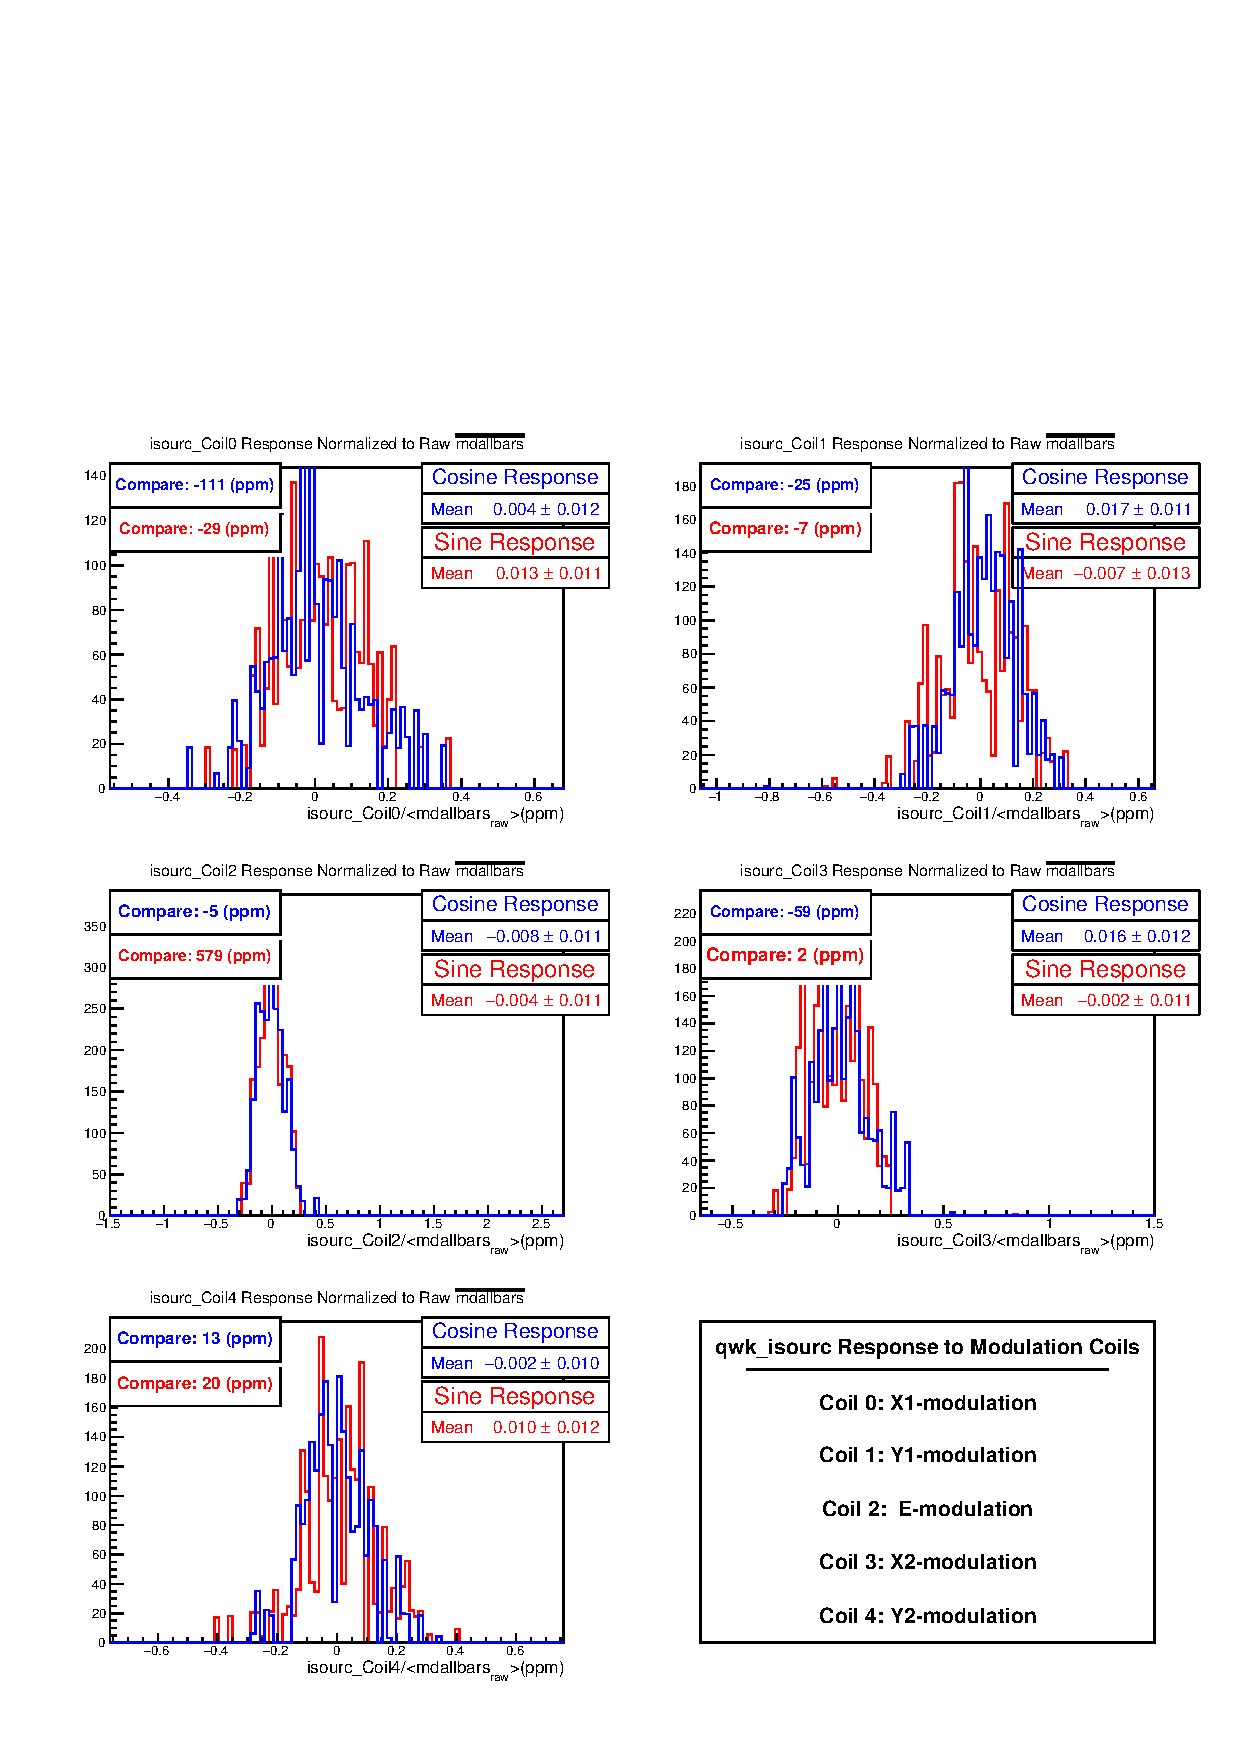
\includegraphics[width=6in]{./Pictures/isourc_coeff.pdf}
\caption{\label{fig:isourc}Response of ``qwk\_isourc'', a current source located in detector hut in the experimental hall and fed through same pre-amplifier and electronics chain as the main detector. Responses shown are normalized to raw MDallbars mean (not normalized to current) for purposes of direct comparison with the MDallbars response given in the ``Compare'' text boxes. The average raw MDallbars value during this period was 5.3~V and the raw isourc value was 8.5~V. As usual, ``Sine'' and ``Cosine'' are the amplitudes of the responses in phase with the modulation coils and 90 degrees out of phase respectively.}
\end{figure}
\begin{figure}[ht]
\centering
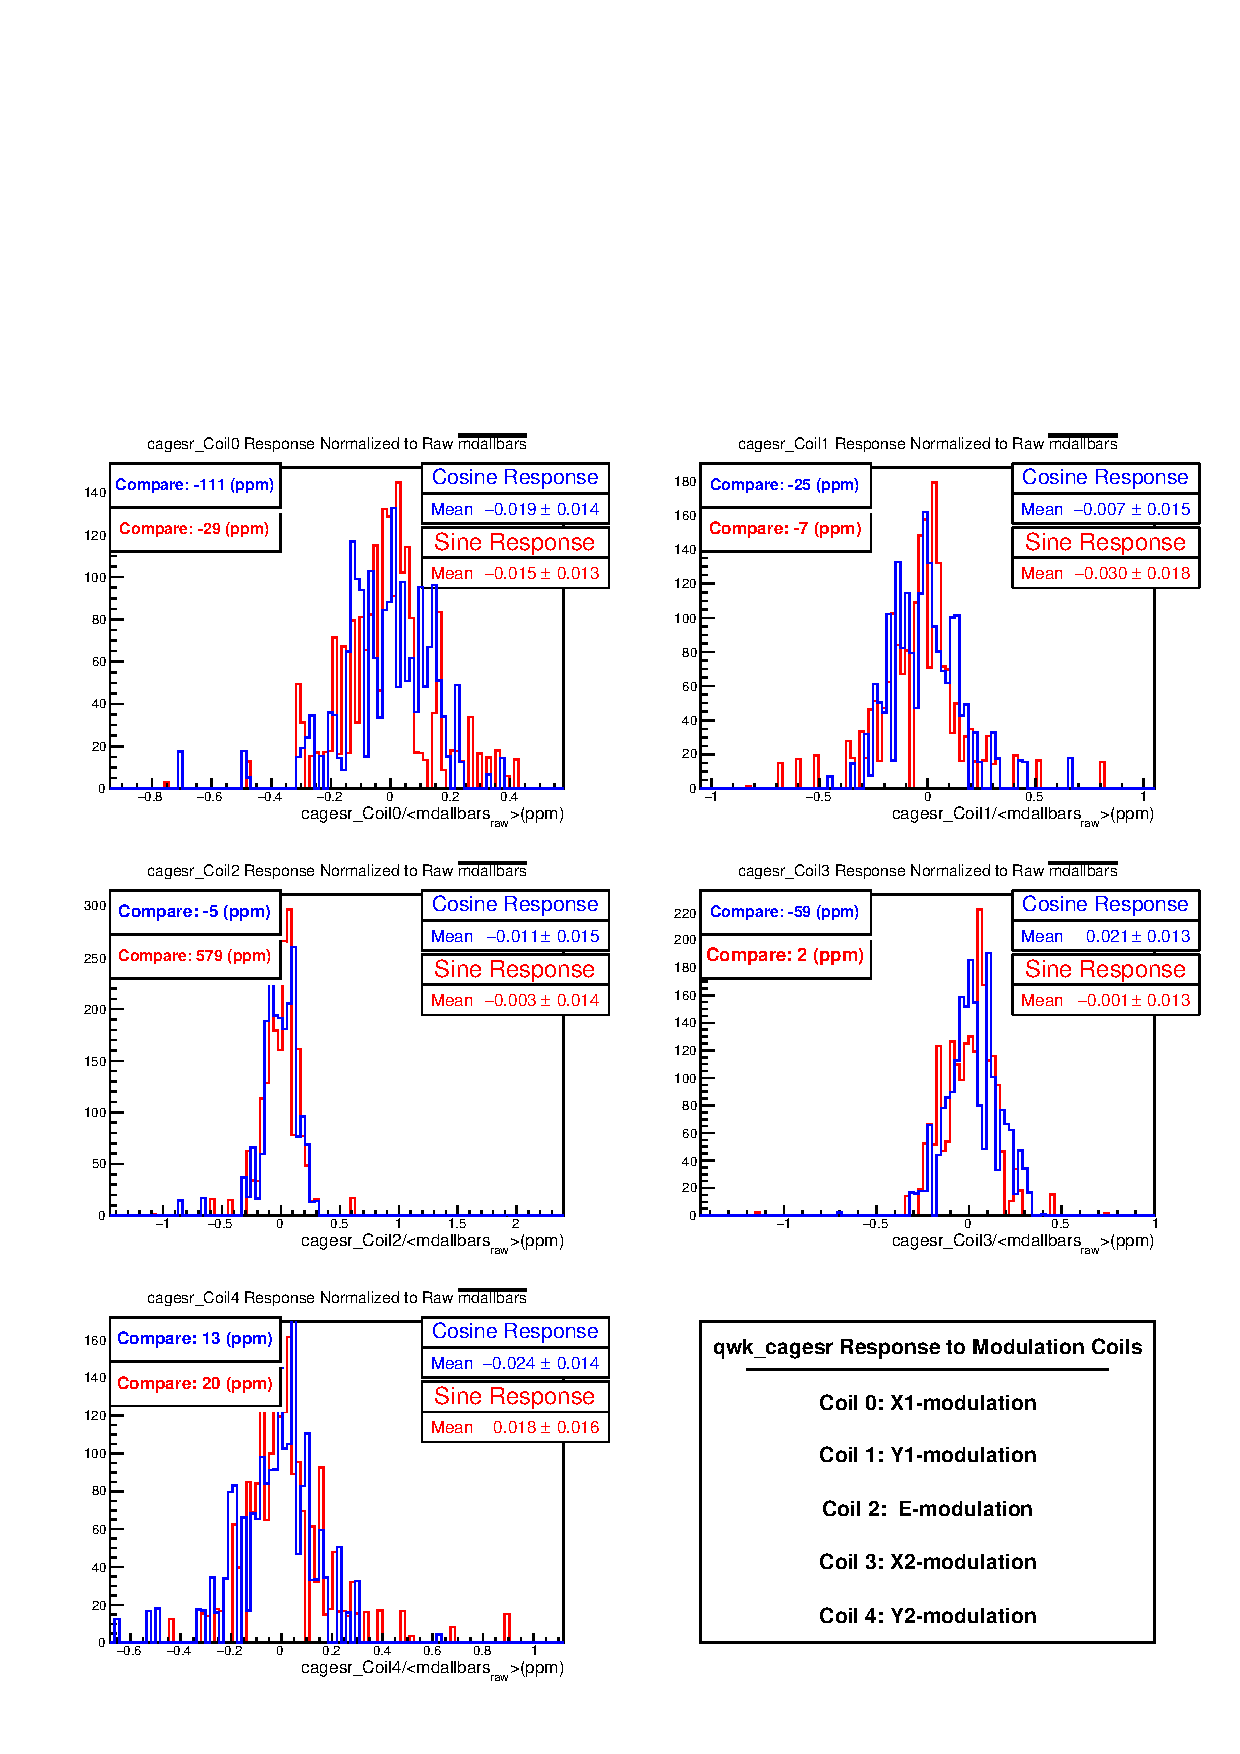
\includegraphics[width=6in]{./Pictures/cagesr_coeff.pdf}
\caption{\label{fig:cagesr}Response of ``qwk\_cagesr'', a battery located in the ``cage''in the Counting House that housed main experimental DAQ electronics. This battery was read out using one of the extra channels used to read out the main detector. The responses shown are normalized to raw MDallbars mean (not normalized to current) for purposes of direct comparison with the MDallbars response given in the ``Compare'' text boxes.  The average raw MDallbars value during this period was 5.3~V and the raw cagesr value was 5.8~V. As usual, ``Sine'' and ``Cosine'' are the amplitudes of the responses in phase with the modulation coils and 90 degrees out of phase respectively.}
\end{figure}
\FloatBarrier

\subsubsection{Differences in Prescribed Corrections}
With information from 10 coils and many beam monitors and with the analysis determining only 5 detector to monitor slopes, there are many combinations of coils and monitors from which the requisite information could be obtained (see Table \ref{tab:coil_nomenclature} for definition of terms). In this section the total correction prescribed by analyses using different coil and monitor sets is investigated. The following constraints must be kept in mind when selecting different sets:
\begin{itemize}
\item{Both monitors and coil sets must adequately span the five dimensions of beam distortion space. That is to say that any set of coils must adequately modulate the beam in all five dimensions and any set of monitors must be able to collectively resolve those five dimensions. }
\item{There are four X-type (horizontal direction) modulation coils and four Y-type (vertical direction) modulation coils. Any useful coil selection must have at a minimum two X-type coils and two Y-type coils. Leaving out any one X-type or Y-type coil gives a total of 8 possible sets. Leaving out any two X-type or two Y-type coils gives a further 12 sets for a total of 20 possible coil sets in addition to the full 10-Coil analysis. Not all of these are guaranteed to have adequate information to provide useful correction slopes.}
\item{There is one E-type (energy) modulation coil. A second but small out-of-phase sensitivity exists for energy as well, but is so small relative to the in-phase energy modulation coil that it is considered negligible and, in fact, its source is not well understood. Omitting the out-of-phase energy coil (Coil 7) makes almost no difference in the analysis but any analysis omitting the large in-phase energy modulation coil (Coil 2) should be considered critically due to lack of energy resolution. Three sets, omitting either in-phase or out-of-phase or omitting both can be considered keeping in mind that most of the energy information will be lost when the in-phase response is omitted. With FFB active during X and Y-type modulations, energy responses will still be measured in the other modulation coils although not nearly as well.}
\item{Although analyses removing 3, 4 and 5 coils are also possible, only a limited number of these will be investigated as evidence is provided for their utility.}
\item{When two coils are removed from either the X-type or Y-type directions, the utility of the redundancy cross-check is lost. In the 5-coil analysis this lack of redundancy was apparent in the precisely zero residuals. When the redundancy cross-check is lost, clues as to the success or failure of the analysis must be provided by other methods (see Section \ref{sctn:residual_correlations}).}
\item{Differences in monitor resolution of the beam parameters will mean that the width of the detector correction will depend upon the monitor set chosen. The monitor set of choice for the modulation analysis are the four target variables and the beam position monitor BPM3c12X because they are particularly well suited for resolving the five dimensions of beam modulation (see Section \ref{sctn:lin_reg} for definition of these monitors). Different monitor sets are expected to yield corrections consistent with each other within the expected statistical deviation from additional detector width associated with differences in monitor resolution.}
\end{itemize}

Tables \ref{tab:run1_dithering_corrections_table} and \ref{tab:run2_dithering_corrections_table} compare the corrections for Runs 1 and 2 for analyses utilizing different coil sets. Coil sets simultaneously omitting coils 0 and 3 and coils 5 and 8 were removed from the comparisons for Run 2 because omitting these coils from the analysis produced sections of data with insufficient information for extraction of useful correction slopes. The results shown are averaged over Wien states weighted by the main detector average asymmetry (MDallbars) errors\footnote{The error weights are the runlet-level (4-5 minutes of data) inverse variance of the MDallbars asymmetry divided by the number of quartets in the runlet: $w_{runlet}=\frac{1}{\sigma_{runlet}^2/N}$}. It becomes apparent, especially in Run 1, that there is a large disparity in the corrections prescribed by analyses with different coil sets. A careful look at the tables shows that omitting coil 3 creates the worst outliers. All coils sets considered invalid are shown as grayed-out in advance of evidence of their unreliability provided in Section \ref{sctn:residual_correlations}.

As previously explained in Section \ref{sctn:electron_source}, \Qs utilized two different slow reversals to cancel out certain types of false asymmetries: 1) half-wave plate insertion and removal on an 8 hour timescale to flip electron source laser helicity;  and  2) monthly double Wien filter reversal of the electron beam helicity relative to its helicity coming off the photo-cathode. With these slow reversal techniques in place, it is not inconceivable that inconsistencies apparent in the modulation could be created by an effect that largely cancels under these reversal, producing the proper average correction. The corrections for Run 2 in Table \ref{tab:run2_dithering_corrections_table} seem to indicate that this type of cancelation is happening and producing consistent average corrections at the $\pm1$~ppb level across all dithering schemes. However, for Run 1 the range of average corrections is a much larger $\pm 6$~ppb. This range helps provide a scale for the effect of inconsistencies in the modulation analysis on the physics asymmetry correction.  

\begin{table}[!h]

\caption{Run 1 dithering corrections for MDallbars asymmetry compared for different coil selections. Grayed-out sets often seen to be outliers are sets considered suspect for reasons investigated in Section \ref{sctn:residual_correlations}.}
\begin{center}
\begin{tabular}[h]{|l||c|c|c|c|c||c|}\hline
Dithering& Wien 1& Wien 2& Wien 3& Wien 4& Wien 5& Total\\
~Scheme&(ppb)&(ppb)&(ppb)&(ppb)&(ppb)&(ppb)\\\hline\hline
10-Coil& -24.1& +3.4& -44.6& -16.8& -17.5& -19.2\\\hline
{\color{Gray}Omit0,3}&{\color{Gray} -36.9}&{\color{Gray} -51.0}&{\color{Gray} -79.5}&{\color{Gray} -21.1}&{\color{Gray} -25.3}&{\color{Gray} -43.8}\\\hline
Omit0,5& -19.2& +21.6& -43.9& -16.9& -14.9& -13.6\\\hline
{\color{Gray}Omit0,8}&{\color{Gray} -16.1}&{\color{Gray} +21.8}&{\color{Gray} -68.8}&{\color{Gray} -24.6}&{\color{Gray} -16.0}&{\color{Gray} -20.2}\\\hline
{\color{Gray}Omit3,5}&{\color{Gray} -53.3}&{\color{Gray} -49.8}&{\color{Gray} -59.0}&{\color{Gray} -16.4}&{\color{Gray} -16.8}&{\color{Gray} -38.9}\\\hline
{\color{Gray}Omit3,8}&{\color{Gray} -88.7}&{\color{Gray} -102.7}&{\color{Gray} -77.6}&{\color{Gray} -22.0}&{\color{Gray} -19.3}&{\color{Gray} -62.3}\\\hline
{\color{Gray}Omit5,8}&{\color{Gray} -10.0}&{\color{Gray} +22.3}&{\color{Gray} -37.9}&{\color{Gray} -16.1}&{\color{Gray} -17.2}&{\color{Gray} -11.0}\\\hline
{\color{Gray}Omit1,4}&{\color{Gray} -28.3}&{\color{Gray} +2.6}&{\color{Gray} -61.2}&{\color{Gray} +11.7}&{\color{Gray} -99.2}&{\color{Gray} -34.1}\\\hline
Omit1,6& -19.5& +7.4& -44.5& -15.8& -17.1& -17.3\\\hline
Omit1,9& -23.9& +3.8& -44.6& -17.2& -17.2& -19.1\\\hline
Omit4,6& -46.0& +4.5& -44.5& -15.3& -17.8& -22.0\\\hline
Omit4,9& -17.3& +1.7& -44.7& -17.4& -18.0& -18.9\\\hline
Omit6,9& -23.6& -1.3& -41.9& -7.4& -12.1& -16.7\\\hline
Omit2,7& -16.6& -2.9& -53.1& -17.9& -19.3& -22.0\\\hline
Omit 0& -16.4& +19.3& -55.9& -20.5& -16.9& -17.4\\\hline
Omit 1& -24.2& +3.6& -44.8& -16.9& -17.3& -19.2\\\hline
Omit 2& -14.8& -6.2& -47.3& -15.2& -16.6& -20.1\\\hline
{\color{Gray}Omit 3}&{\color{Gray} -84.0}&{\color{Gray} -95.8}&{\color{Gray} -75.4}&{\color{Gray} -20.7}&{\color{Gray} -19.2}&{\color{Gray} -59.2}\\\hline
Omit 4& -23.7& +2.5& -44.7& -16.7& -18.2& -19.5\\\hline
Omit 5& -11.5& +20.4& -38.7& -16.1& -17.0& -11.8\\\hline
Omit 6& -24.0& +3.3& -44.5& -15.6& -17.2& -18.9\\\hline
Omit 7& -24.1& +3.4& -44.7& -17.1& -17.5& -19.3\\\hline
Omit 8& -23.5& +4.3& -44.3& -16.9& -17.7& -18.9\\\hline
Omit 9& -23.8& +3.1& -44.6& -17.2& -17.5& -19.3\\\hline
\end{tabular}
\end{center}
\label{tab:run1_dithering_corrections_table}
\end{table}


\begin{table}[!h]

\caption{Run 2 dithering corrections for MDallbars asymmetry compared for different coil selections. Grayed-out sets often seen to be outliers are sets considered suspect for reasons investigated in Section \ref{sctn:residual_correlations}.}
\begin{center}
\begin{tabular}[h]{|l||c|c|c|c|c|c||c|}\hline
Dithering& Wien 6& Wien 7& Wien 8a& Wien 8b& Wien 9a& Wien 9b& Total\\
~Scheme&(ppb)&(ppb)&(ppb)&(ppb)&(ppb)&(ppb)&(ppb)\\\hline\hline
10-Coil& -25.5& +35.6& -12.3& -4.3& +2.0& +1.3& -1.7\\\hline
Omit0,5& -24.7& +36.0& -13.9& -5.3& +1.7& +0.2& -2.4\\\hline
{\color{Gray}Omit0,8}&{\color{Gray} -27.2}&{\color{Gray} +36.4}&{\color{Gray} -33.8}&{\color{Gray} +0.9}&{\color{Gray} -0.1}&{\color{Gray} +0.2}&{\color{Gray} -5.0}\\\hline
{\color{Gray}Omit3,5}&{\color{Gray} -26.3}&{\color{Gray} +36.3}&{\color{Gray} -17.4}&{\color{Gray} -5.6}&{\color{Gray} +2.9}&{\color{Gray} +4.5}&{\color{Gray} -1.8}\\\hline
{\color{Gray}Omit3,8}&{\color{Gray} -29.3}&{\color{Gray} +38.5}&{\color{Gray} -23.6}&{\color{Gray} -1.2}&{\color{Gray} +3.0}&{\color{Gray} +13.9}&{\color{Gray} +0.2}\\\hline
{\color{Gray}Omit1,4}&{\color{Gray} -14.2}&{\color{Gray} +31.3}&{\color{Gray} -40.8}&{\color{Gray} -11.0}&{\color{Gray} -2.2}&{\color{Gray} -1.0}&{\color{Gray} -8.0}\\\hline
Omit1,6& -25.7& +37.6& -12.1& -4.4& +1.9& +1.3& -1.6\\\hline
Omit1,9& -25.5& +35.6& -12.2& -4.2& +2.0& +1.3& -1.7\\\hline
Omit4,6& -25.4& +37.8& -12.2& -4.2& +1.9& +1.5& -1.5\\\hline
Omit4,9& -25.1& +35.7& -12.5& -4.4& +1.9& +1.4& -1.8\\\hline
Omit6,9& -27.3& +36.1& -10.8& -3.7& +1.9& +1.5& -1.5\\\hline
Omit2,7& -28.8& +53.2& -13.0& -5.4& +2.3& +3.3& -0.5\\\hline
{\color{Gray}Omit 0}&{\color{Gray} -26.2}&{\color{Gray} +37.8}&{\color{Gray} -23.4}&{\color{Gray} -1.8}&{\color{Gray} +0.4}&{\color{Gray} +1.0}&{\color{Gray} -3.3}\\\hline
Omit 1& -25.3& +36.5& -12.3& -4.2& +2.0& +1.3& -1.6\\\hline
Omit 2& -27.0& +33.1& -12.9& -5.3& +2.2& +2.7& -2.0\\\hline
{\color{Gray}Omit 3}&{\color{Gray} -29.1}&{\color{Gray} +37.9}&{\color{Gray} -22.5}&{\color{Gray} -1.8}&{\color{Gray} +2.8}&{\color{Gray} +7.9}&{\color{Gray} -1.2}\\\hline
Omit 4& -25.1& +36.1& -12.6& -4.3& +1.9& +1.4& -1.7\\\hline
Omit 5& -24.6& +35.4& -9.3& -5.2& +2.2& +1.0& -1.4\\\hline
Omit 6& -25.4& +37.3& -12.1& -4.2& +1.9& +1.4& -1.6\\\hline
Omit 7& -25.5& +35.7& -12.3& -4.3& +2.0& +1.4& -1.7\\\hline
Omit 8& -25.5& +37.7& -12.0& -4.1& +2.0& +1.4& -1.5\\\hline
Omit 9& -25.2& +35.7& -12.2& -4.2& +2.0& +1.3& -1.7\\\hline
\end{tabular}
\end{center}
\label{tab:run2_dithering_corrections_table}
\end{table}

Another useful set of cross-checks used in parity-violation experiments are null asymmetries which are a measurement of the differences cancelled by slow reversals. Null asymmetries that are small or consistent with zero are a good indication that there are not significant sources of systematic false asymmetries being cancelled by the slow helicity reversal. If the source of the cancellations is understood, it is not necessary that the null be consistent with 0. After all, one of the purposes of slow helicity reversal is to cancel small false asymmetries. However, large cancellations of effects not well understood sometimes requires the addition of a systematic error. For this reason it is appropriate to look at beam modulation corrections prescribed to null asymmetries as well. For the purposes of \Qs there are three slow helicity-reversal mechanisms: the insertable half-wave plate (IHWP), the double Wien filter, and the g-2 reversal from traveling around the accelerator.

The two most important null asymmetries relevant to this study are defined as follows:
\begin{itemize}
\item{{\bf ``IHWP+Spin-reversal'' Null}~~~~~$\left[\frac{A_{IN}^{raw}+A_{OUT}^{raw}}{2}\right]$:\\ This null is the average asymmetry of both half-wave plate (HWP) states with no sign corrections applied to the asymmetries for any of the three slow reversals. The parity-violating physics asymmetry is expected to cancel leaving false asymmetries due to effects such as electrical pickup of the helicity reversal signal or mechanical effects such as lensing in the electron source Pockels cell. }
\item{{\bf ``IHWP-only'' Null}~~~~$\left[\frac{Sign(A_{IN}^{raw})-Sign(A_{OUT}^{raw})}{2}\right]$:\\ This null is the difference between average asymmetries of IHWP states, each individually sign-corrected for all slow reversals. By sign-correcting for all slow reversals and then taking the difference between the two IHWP states, the effect of the IHWP reversal is isolated. This null reveals false asymmetries that cancel with the IHWP reversal but survive the other slow reversal cancelations.}
\end{itemize}

Tables \ref{tab:run1_null_corrections_table} and \ref{tab:run2_null_corrections_table} show the range of corrections for Runs 1 and 2 respectively to the ``IHWP+Spin-reversal'' null asymmetry provided by analyses with various coil selections. Tables \ref{tab:run1_ihwp_only_null_corrections_table} and \ref{tab:run2_ihwp_only_null_corrections_table} show the analogous range of corrections to the ``IHWP-only'' null. From these tables one can easily observe: 1) that the inconsistency in the various modulation corrections is more apparent in the null asymmetry corrections than in the physics asymmetry corrections; and 2) variations in the null asymmetries are at least as large if not larger in Run 2 than they are in Run 1 even though the spread in the physics asymmetry corrections is much smaller.

Inconsistencies on the order of 30~ppb in the null asymmetry corrections using various coil selections help give a scale to the issue with the beam modulation analysis. If \Qs were not set up to benefit from slow reversal cancellation or if a single IHWP state were modulation-corrected, there would be discrepancies of tens of ppb between different schemes. This does not mean that there is an error in the modulation correction slopes that is IHWP-correlated. The modulation correction comes from the product of the correction slopes and monitor differences and this discrepancy in the null mainly points to the slow-reversal cancellation of monitor differences, that is, the helicity-correlated beam properties measured in the monitors. Utilizing the full cancellation of slow reversals allows the assignment of a much smaller systematic error for this discrepancy.


\begin{table}[!h]
%table made by ~/thesis_plot_macros/MakeDitheringCorrectionsTable.C
\caption{Run 1 dithering corrections to ``IHWP-only'' null asymmetry for various coil selections. Grayed-out sets considered suspect  for reasons investigated in Section \ref{sctn:residual_correlations}.}
\begin{center}
\begin{tabular}[h]{|l||c|c|c|c|c||c|}\hline
Dithering& Wien 1& Wien 2& Wien 3& Wien 4& Wien 5& Total\\
~Scheme&(ppb)&(ppb)&(ppb)&(ppb)&(ppb)&(ppb)\\\hline\hline
10-Coil& -14.6& -13.1& +38.5& -115.8& +6.3& -19.0\\\hline
{\color{Gray}Omit0,3}&{\color{Gray} -14.3}&{\color{Gray} -76.2}&{\color{Gray} +76.8}&{\color{Gray} -312.0}&{\color{Gray} -203.6}&{\color{Gray} -107.1}\\\hline
Omit0,5& -6.3& -9.7& +37.2& -102.1& +8.8& -13.7\\\hline
{\color{Gray}Omit0,8}&{\color{Gray} -6.4}&{\color{Gray} -15.1}&{\color{Gray} +57.3}&{\color{Gray} -128.9}&{\color{Gray} -113.6}&{\color{Gray} -39.6}\\\hline
{\color{Gray}Omit3,5}&{\color{Gray} -27.1}&{\color{Gray} -58.8}&{\color{Gray} +53.6}&{\color{Gray} -206.5}&{\color{Gray} -81.6}&{\color{Gray} -65.7}\\\hline
{\color{Gray}Omit3,8}&{\color{Gray} -42.9}&{\color{Gray} -115.6}&{\color{Gray} +72.9}&{\color{Gray} -274.6}&{\color{Gray} -181.9}&{\color{Gray} -112.3}\\\hline
{\color{Gray}Omit5,8}&{\color{Gray} -9.4}&{\color{Gray} +10.4}&{\color{Gray} +32.0}&{\color{Gray} -91.4}&{\color{Gray} +47.0}&{\color{Gray} -0.5}\\\hline
{\color{Gray}Omit1,4}&{\color{Gray} -16.2}&{\color{Gray} -30.3}&{\color{Gray} +33.7}&{\color{Gray} -409.9}&{\color{Gray} -74.7}&{\color{Gray} -97.2}\\\hline
Omit1,6& -36.3& +2.9& +38.5& -113.6& +6.1& -17.6\\\hline
Omit1,9& -14.1& -13.1& +38.5& -114.8& +6.4& -18.7\\\hline
Omit4,6& -16.7& -13.7& +38.6& -116.3& +5.6& -20.5\\\hline
Omit4,9& -15.3& -13.4& +38.5& -118.7& +5.9& -19.6\\\hline
Omit6,9& -15.8& -17.5& +39.3& -85.1& +1.2& -15.2\\\hline
Omit2,7& -7.5& -18.4& +45.8& -124.5& +19.8& -16.6\\\hline
Omit 0& -6.6& -13.0& +47.2& -119.0& -56.7& -28.3\\\hline
Omit 1& -14.3& -13.3& +38.7& -114.8& +6.4& -18.8\\\hline
Omit 2& -6.1& -19.9& +40.9& -119.0& +6.7& -19.4\\\hline
{\color{Gray}Omit 3}&{\color{Gray} -40.0}&{\color{Gray} -108.7}&{\color{Gray} +70.7}&{\color{Gray} -264.0}&{\color{Gray} -169.2}&{\color{Gray} -105.8}\\\hline
Omit 4& -15.0& -13.4& +38.5& -118.4& +5.8& -19.7\\\hline
Omit 5& -10.1& +8.3& +32.7& -95.1& +41.3& -2.9\\\hline
Omit 6& -15.7& -13.1& +38.6& -114.0& +5.9& -18.9\\\hline
Omit 7& -14.6& -13.1& +38.6& -115.6& +6.4& -18.9\\\hline
Omit 8& -14.3& -12.2& +38.2& -114.2& +8.8& -18.0\\\hline
Omit 9& -14.6& -13.3& +38.5& -115.6& +6.2& -19.0\\\hline
\end{tabular}
\end{center}
\label{tab:run1_ihwp_only_null_corrections_table}
\end{table}

\begin{table}[!h]

\caption{Run 2 dithering corrections to ``IHWP-only'' null asymmetry for various coil selections. Grayed-out sets considered suspect  for reasons investigated in Section \ref{sctn:residual_correlations}.}
\begin{center}
\begin{tabular}[h]{|l||c|c|c|c|c|c||c|}\hline
Dithering& Wien 6& Wien 7& Wien 8a& Wien 8b& Wien 9a& Wien 9b& Total\\
~Scheme&(ppb)&(ppb)&(ppb)&(ppb)&(ppb)&(ppb)&(ppb)\\\hline\hline
10-Coil& +24.6& +129.1& -35.9& -22.6& -0.9& -8.4& +0.6\\\hline
Omit0,5& +24.1& +127.6& -39.9& -23.9& -3.9& -17.3& -3.3\\\hline
{\color{Gray}Omit0,8}&{\color{Gray} +19.1}&{\color{Gray} +142.8}&{\color{Gray} -145.4}&{\color{Gray} -93.4}&{\color{Gray} -38.6}&{\color{Gray} -35.3}&{\color{Gray} -44.0}\\\hline
{\color{Gray}Omit3,5}&{\color{Gray} +25.2}&{\color{Gray} +129.1}&{\color{Gray} -75.4}&{\color{Gray} -41.2}&{\color{Gray} -5.2}&{\color{Gray} -24.4}&{\color{Gray} -13.4}\\\hline
{\color{Gray}Omit3,8}&{\color{Gray} +28.7}&{\color{Gray} +137.1}&{\color{Gray} -132.3}&{\color{Gray} -77.2}&{\color{Gray} -14.8}&{\color{Gray} -58.3}&{\color{Gray} -37.8}\\\hline
{\color{Gray}Omit1,4}&{\color{Gray} -2.4}&{\color{Gray} +129.5}&{\color{Gray} -16.9}&{\color{Gray} -26.7}&{\color{Gray} -7.6}&{\color{Gray} -6.6}&{\color{Gray} -1.1}\\\hline
Omit1,6& +24.8& +130.4& -35.3& -21.2& -0.5& -8.7& +1.1\\\hline
Omit1,9& +24.6& +129.3& -35.8& -22.6& -1.0& -8.7& +0.5\\\hline
Omit4,6& +25.0& +133.1& -35.4& -22.0& -0.6& -8.5& +1.2\\\hline
Omit4,9& +24.8& +131.5& -35.7& -23.2& -1.3& -8.6& +0.6\\\hline
Omit6,9& +28.7& +131.3& -32.9& -19.5& -0.2& -8.0& +2.4\\\hline
Omit2,7& +29.2& +100.3& -34.0& -20.0& -0.4& -5.2& +0.5\\\hline
{\color{Gray}Omit 0}&{\color{Gray} +20.8}&{\color{Gray} +135.7}&{\color{Gray} -89.8}&{\color{Gray} -59.5}&{\color{Gray} -18.1}&{\color{Gray} -24.1}&{\color{Gray} -21.9}\\\hline
Omit 1& +24.8& +130.0& -36.0& -22.7& -0.9& -8.7& +0.6\\\hline
Omit 2& +27.8& +129.1& -34.1& -20.3& -0.8& -6.6& +2.1\\\hline
{\color{Gray}Omit 3}&{\color{Gray} +28.6}&{\color{Gray} +135.1}&{\color{Gray} -123.0}&{\color{Gray} -72.2}&{\color{Gray} -12.4}&{\color{Gray} -37.7}&{\color{Gray} -30.2}\\\hline
Omit 4& +24.8& +129.5& -35.9& -23.2& -1.1& -8.6& +0.4\\\hline
Omit 5& +24.5& +126.1& -15.9& -10.2& +3.0& -4.2& +7.5\\\hline
Omit 6& +25.0& +130.4& -35.5& -21.7& -0.6& -8.2& +1.1\\\hline
Omit 7& +24.6& +129.1& -35.9& -22.6& -0.9& -8.4& +0.6\\\hline
Omit 8& +24.6& +132.8& -33.7& -21.5& -0.1& -6.9& +1.9\\\hline
Omit 9& +24.8& +131.7& -35.8& -22.7& -0.9& -8.4& +0.8\\\hline
\end{tabular}
\end{center}
\label{tab:run2_ihwp_only_null_corrections_table}
\end{table}

\begin{table}[!h]
%table made by ~/thesis_plot_macros/MakeDitheringCorrectionsTable.C
\caption{Run 1 dithering corrections to ``IHWP+Spin-reversal'' null asymmetry for various coil selections. Grayed-out sets considered suspect  for reasons investigated in Section \ref{sctn:residual_correlations}.}
\begin{center}
\begin{tabular}[h]{|l||c|c|c|c|c||c|}\hline
Dithering& Wien 1& Wien 2& Wien 3& Wien 4& Wien 5& Total\\
~Scheme&(ppb)&(ppb)&(ppb)&(ppb)&(ppb)&(ppb)\\\hline\hline
10-Coil& -14.6& +13.1& +38.5& +115.8& +6.3& +33.4\\\hline
{\color{Gray}Omit0,3}&{\color{Gray} -14.3}&{\color{Gray} +76.2}&{\color{Gray} +76.8}&{\color{Gray} +312.0}&{\color{Gray} -203.6}&{\color{Gray} +56.1}\\\hline
Omit0,5& -6.3& +9.7& +37.2& +102.1& +8.8& +30.9\\\hline
{\color{Gray}Omit0,8}&{\color{Gray} -6.4}&{\color{Gray} +15.1}&{\color{Gray} +57.3}&{\color{Gray} +128.9}&{\color{Gray} -113.6}&{\color{Gray} +18.2}\\\hline
{\color{Gray}Omit3,5}&{\color{Gray} -27.1}&{\color{Gray} +58.8}&{\color{Gray} +53.6}&{\color{Gray} +206.5}&{\color{Gray} -81.6}&{\color{Gray} +46.7}\\\hline
{\color{Gray}Omit3,8}&{\color{Gray} -42.9}&{\color{Gray} +115.6}&{\color{Gray} +72.9}&{\color{Gray} +274.6}&{\color{Gray} -181.9}&{\color{Gray} +55.7}\\\hline
{\color{Gray}Omit5,8}&{\color{Gray} -9.4}&{\color{Gray} -10.4}&{\color{Gray} +32.0}&{\color{Gray} +91.4}&{\color{Gray} +47.0}&{\color{Gray} +30.4}\\\hline
{\color{Gray}Omit1,4}&{\color{Gray} -16.2}&{\color{Gray} +30.3}&{\color{Gray} +33.7}&{\color{Gray} +409.9}&{\color{Gray} -74.7}&{\color{Gray} +83.6}\\\hline
Omit1,6& -36.3& -2.9& +38.5& +113.6& +6.1& +26.3\\\hline
Omit1,9& -14.1& +13.1& +38.5& +114.8& +6.4& +33.3\\\hline
Omit4,6& -16.7& +13.7& +38.6& +116.3& +5.6& +32.4\\\hline
Omit4,9& -15.3& +13.4& +38.5& +118.7& +5.9& +34.2\\\hline
Omit6,9& -15.8& +17.5& +39.3& +85.1& +1.2& +27.3\\\hline
Omit2,7& -7.5& +18.4& +45.8& +124.5& +19.8& +42.0\\\hline
Omit 0& -6.6& +13.0& +47.2& +119.0& -56.7& +24.7\\\hline
Omit 1& -14.3& +13.3& +38.7& +114.8& +6.4& +33.3\\\hline
Omit 2& -6.1& +19.9& +40.9& +119.0& +6.7& +37.9\\\hline
{\color{Gray}Omit 3}&{\color{Gray} -40.0}&{\color{Gray} +108.7}&{\color{Gray} +70.7}&{\color{Gray} +264.0}&{\color{Gray} -169.2}&{\color{Gray} +54.4}\\\hline
Omit 4& -15.0& +13.4& +38.5& +118.4& +5.8& +33.9\\\hline
Omit 5& -10.1& -8.3& +32.7& +95.1& +41.3& +30.6\\\hline
Omit 6& -15.7& +13.1& +38.6& +114.0& +5.9& +32.8\\\hline
Omit 7& -14.6& +13.1& +38.6& +115.6& +6.4& +33.4\\\hline
Omit 8& -14.3& +12.2& +38.2& +114.2& +8.8& +33.3\\\hline
Omit 9& -14.6& +13.3& +38.5& +115.6& +6.2& +33.4\\\hline
\end{tabular}
\end{center}
\label{tab:run1_null_corrections_table}
\end{table}

\begin{table}[!h]

\caption{Run 2 dithering corrections to ``IHWP+Spin-reversal'' null asymmetry for various coil selections. Grayed-out sets considered suspect for reasons investigated in Section \ref{sctn:residual_correlations}.}
\begin{center}
\begin{tabular}[h]{|l||c|c|c|c|c|c||c|}\hline
Dithering& Wien 6& Wien 7& Wien 8a& Wien 8b& Wien 9a& Wien 9b& Total\\
~Scheme&(ppb)&(ppb)&(ppb)&(ppb)&(ppb)&(ppb)&(ppb)\\\hline\hline
10-Coil& +24.6& -129.1& -35.9& -22.6& +0.9& +8.4& -13.9\\\hline
Omit0,5& +24.1& -127.6& -39.9& -23.9& +3.9& +17.3& -11.8\\\hline
{\color{Gray}Omit0,8}&{\color{Gray} +19.1}&{\color{Gray} -142.8}&{\color{Gray} -145.4}&{\color{Gray} -93.6}&{\color{Gray} +38.6}&{\color{Gray} +35.3}&{\color{Gray} -27.9}\\\hline
{\color{Gray}Omit3,5}&{\color{Gray} +25.2}&{\color{Gray} -129.1}&{\color{Gray} -75.4}&{\color{Gray} -41.3}&{\color{Gray} +5.2}&{\color{Gray} +24.4}&{\color{Gray} -18.1}\\\hline
{\color{Gray}Omit3,8}&{\color{Gray} +28.7}&{\color{Gray} -137.1}&{\color{Gray} -132.3}&{\color{Gray} -77.4}&{\color{Gray} +14.8}&{\color{Gray} +58.4}&{\color{Gray} -22.5}\\\hline
{\color{Gray}Omit1,4}&{\color{Gray} -2.4}&{\color{Gray} -129.5}&{\color{Gray} -16.9}&{\color{Gray} -26.7}&{\color{Gray} +7.6}&{\color{Gray} +6.6}&{\color{Gray} -13.1}\\\hline
Omit1,6& +24.8& -130.4& -35.3& -21.3& +0.5& +8.7& -13.7\\\hline
Omit1,9& +24.6& -129.3& -35.8& -22.6& +1.0& +8.7& -13.8\\\hline
Omit4,6& +25.0& -133.1& -35.4& -22.0& +0.6& +8.5& -14.0\\\hline
Omit4,9& +24.8& -131.5& -35.7& -23.2& +1.3& +8.6& -14.0\\\hline
Omit6,9& +28.7& -131.3& -32.9& -19.5& +0.2& +8.0& -13.0\\\hline
Omit2,7& +29.2& -100.3& -34.0& -20.0& +0.4& +5.2& -11.4\\\hline
{\color{Gray}Omit 0}&{\color{Gray} +20.8}&{\color{Gray} -135.7}&{\color{Gray} -89.8}&{\color{Gray} -59.6}&{\color{Gray} +18.1}&{\color{Gray} +24.1}&{\color{Gray} -21.1}\\\hline
Omit 1& +24.8& -130.0& -36.0& -22.7& +0.9& +8.8& -13.9\\\hline
Omit 2& +27.8& -129.1& -34.1& -20.3& +0.8& +6.6& -13.4\\\hline
{\color{Gray}Omit 3}&{\color{Gray} +28.6}&{\color{Gray} -135.1}&{\color{Gray} -123.0}&{\color{Gray} -72.4}&{\color{Gray} +12.4}&{\color{Gray} +37.8}&{\color{Gray} -25.7}\\\hline
Omit 4& +24.8& -129.5& -35.9& -23.2& +1.1& +8.6& -13.9\\\hline
Omit 5& +24.5& -126.1& -15.9& -10.1& -3.0& +4.2& -10.6\\\hline
Omit 6& +25.0& -130.4& -35.5& -21.8& +0.6& +8.2& -13.9\\\hline
Omit 7& +24.6& -129.1& -35.9& -22.6& +0.9& +8.4& -13.9\\\hline
Omit 8& +24.6& -132.8& -33.7& -21.5& +0.1& +6.9& -14.2\\\hline
Omit 9& +24.8& -131.7& -35.8& -22.7& +0.9& +8.4& -14.1\\\hline
\end{tabular}
\end{center}
\label{tab:run2_null_corrections_table}
\end{table}
\FloatBarrier
To study the effect of varying the set of {\bf monitors} used in the modulation analysis on the detector correction, a full analysis was completed with three different sets of monitors chosen. The first set, hereafter referred to as ``Set A'', was the original default set with the target variables plus BPM3c12X. A second set, hereafter referred to as ``Set B'', comprised the target variables plus an alternate energy-sensitive beam position monitor BPM3p02bY. This BPM is located in the vertically-dispersive region of the Hall C Compton polarimeter and is about 7 times less sensitive to energy shifts than BPM3c12X since its dispersion is only 57~cm compared to the 4.4~m of the Hall C arc at girder 3c12. This choice has a two-fold advantage. First, the dispersive direction of the BPM3p02bY is vertical whereas that of  BPM3c12X is horizontal which might allow potential issues associated with strength sharing between energy and position to be disentangled. Second, this BPM is located 35 meters downstream of BPM3c12 and might be sensitive to additional effects to which BPM3c12X is blind. An example of such an hypothesis which was investigated as a possible source of the modulation inconsistency is electronics pickup of the modulation signal by an air coil magnet on the beamline downstream of BPM3c12. This would create an effect on the beam coherent with the modulation driving signal which would be invisible to BPM3c12X and would likely compromise the validity of the energy correction. Finally, a third set ``Set C'' is composed of five single BPM's named according to the beamline girder on which they are located: BPM3c11X (energy),  BPM3c14X and BPM3h02X (X and X angle), and BPM3c14Y and BPM3h02Y (Y and Y angle). ``Set C'' represents a completely independent set of monitors none of which are included in the Sets A and B. Differences in the widths of the corrections can be expected due to variations in the resolution of the different monitor sets. Set A which uses the average of many BPM's to calculate position and angle on target along with the most sensitive energy BPM is expected to give the smallest correction distribution width since its collective resolution of the five beam parameters is smallest. 

The plots in Figure \ref{fig:compton_bpm_slopes} compare the correction slopes given by analyses using BPM3c12X (Set A) and BPM3p02bY (Set B) as energy monitor. It can easily be seen that monitors sensitive to the dispersive direction of the energy monitor used have much larger slopes due to mixing of energy and position/slope in that direction. During Run 2 (after slug 136), energy slopes using BPM3p02bY are 7-8 times larger than those from BPM3c12X which is roughly the scaling one would expect from the difference in dispersion. During Run 1, the slopes do not appear to scale the same way with dispersion. Since there are no common monitors between Set C and the other two sets, comparison of the slopes for Set C is irrelevant.

\begin{figure}[ht]

\centering
\framebox{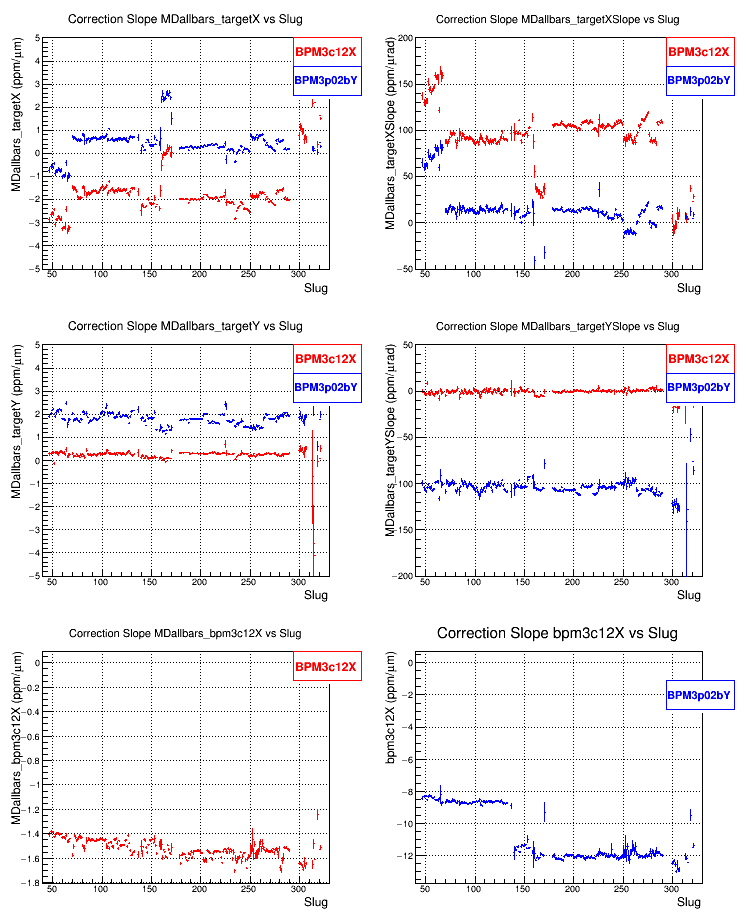
\includegraphics[width=5in]{Pictures/slopes_compton_bpm.png}}
\caption{Comparison of correction slopes from two analyses, one using BPM3c12X as energy monitor and the other using BPM3p02bY.}
\label{fig:compton_bpm_slopes}
\end{figure}

The key issue is whether or not the three sets give statistically consistent results for the magnitude of the corrections. The total correction distributions for the three monitor sets are shown in Figure \ref{fig:correction_distributions}. The width increase from Set A to the other monitor sets is obvious. These distributions are not expected to be normal, so direct statistical comparison of the distributions is not meaningful.
\begin{figure}[ht]

\centering
\framebox{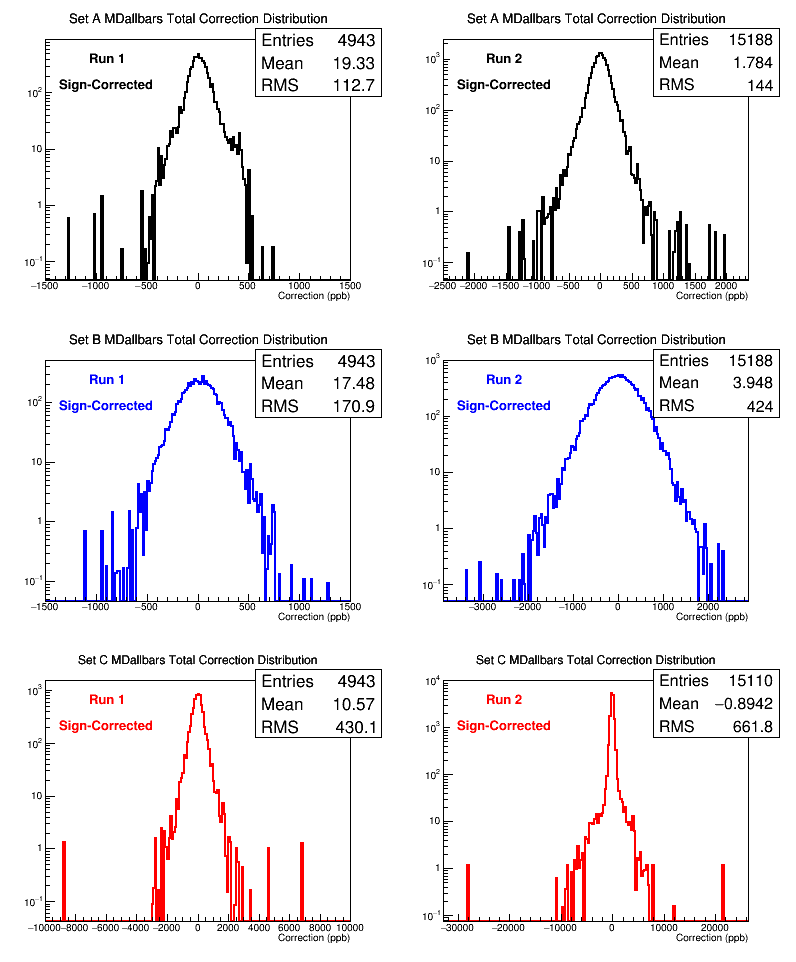
\includegraphics[width=5in]{Pictures/correction_distributions.png}}
\caption{Comparison of total correction  distributions for monitor Sets A, B and C. Each entry in the distributions represents the correction for approximately 5 minutes of data. Distributions are sign-corrected to remove the sign of the slow helicity reversals and are all weighted by the uncorrected ``MDallbars'' inverse variance for purposes of comparison.}
\label{fig:correction_distributions}
\end{figure}
 However, one might expect that the difference between corrections of two Sets to arise solely from differences in monitor resolution or noise which {\it is} statistical. Of course, monitor resolution of the position and angle on target as well as energy can change with beam tune so each difference in the distribution must be normalized to the time-dependent standard deviation of the difference distribution. An estimate of this standard deviation for a given time can be obtained from the quadrature difference of the corrected main detector error given by the two sets for that time period.
 The distribution of these normalized differences is called a pull plot and each entry is given by
\[
\frac{Correction_{(Set~i)}-Correction_{(Set~j)}}{\sqrt{\left|\frac{\sigma_{(Set~i)}^2}{N}-\frac{\sigma_{(Set~j)}^2}{N}\right|}},
\]
where $\sigma_{(Set~i)}$ is the main detector average (MDallbars) asymmetry width after modulation correction with monitor Set~i and $N$ is the number of samples averaged. If the differences in the applied corrections between the two analyses are consistent with statistics, the pull-plot of the distribution of the difference between the two sets will be consistent with a normal distribution with mean 0 and standard deviation 1.\begin{figure}[ht]

\centering
\framebox{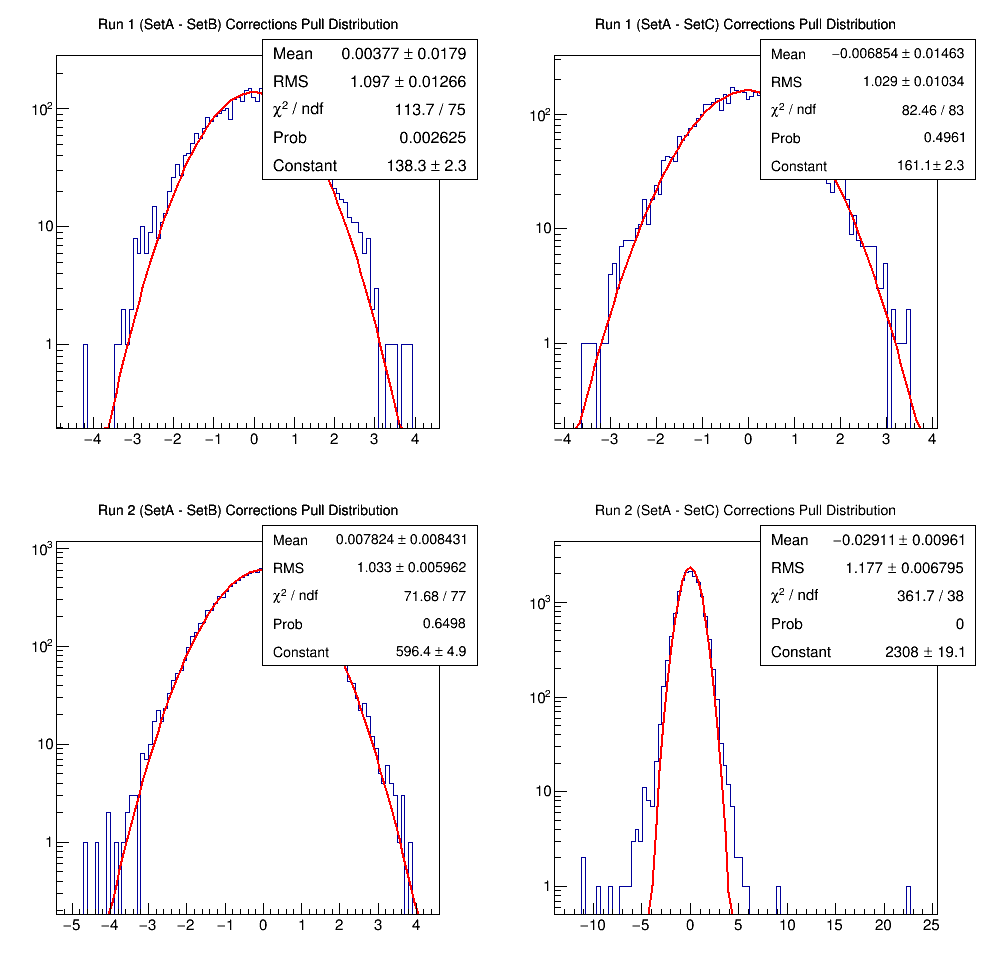
\includegraphics[width=4.5in]{Pictures/runlet_pull_plots.png}}
\caption{Pull plot distributions for difference in corrections provided by monitor Set A and those of Sets B and C. Each entry in the distributions is the average over a ``runlet'' and represents about 5 minutes of data and no sign-correction has been applied. The fit shown is for a Gaussian distribution with mean 0 and standard deviation 1 and with the scale factor as the only free parameter. From the probabilities it is clear that during Run 1 Sets A and C are statistically consistent whereas Sets A and B are not. In Run 2 the opposite appears to be true with Sets A and B statistically consistent and Sets A and C inconsistent.}
\label{fig:runlet_pull_plots}
\end{figure}
 Figure \ref{fig:runlet_pull_plots} shows the pull plot distributions for comparing corrections using monitor Set A with Sets B and C. The pull distributions have been fit with normal distribution curves. The probabilities clearly point to inconsistencies beyond statistics between Sets A and B in Run 1 and between Sets A and C in Run 2 at least at this averaging timescale ($\sim 5$~minutes). On the other hand, the results of Sets A and C are statistically consistent during Run 1 as are Sets A and B during Run 2. The pull plots further indicate that the non-normality of the pull distributions arises from an under-estimated width whereas their means are nearly consistent with 0. 

Over longer averaging periods the inconsistencies between monitor sets disappears. This can be clearly seen in Figure \ref{fig:slug_pull_plots} which shows a set of pull plots similar to those in Figure \ref{fig:runlet_pull_plots} but with each entry in the pull histograms representing the average over  $\sim 8$~hours. The pull distributions indicate that at this timescale all three monitor sets give consistent results within statistics.  
\begin{figure}[ht]

\centering
\framebox{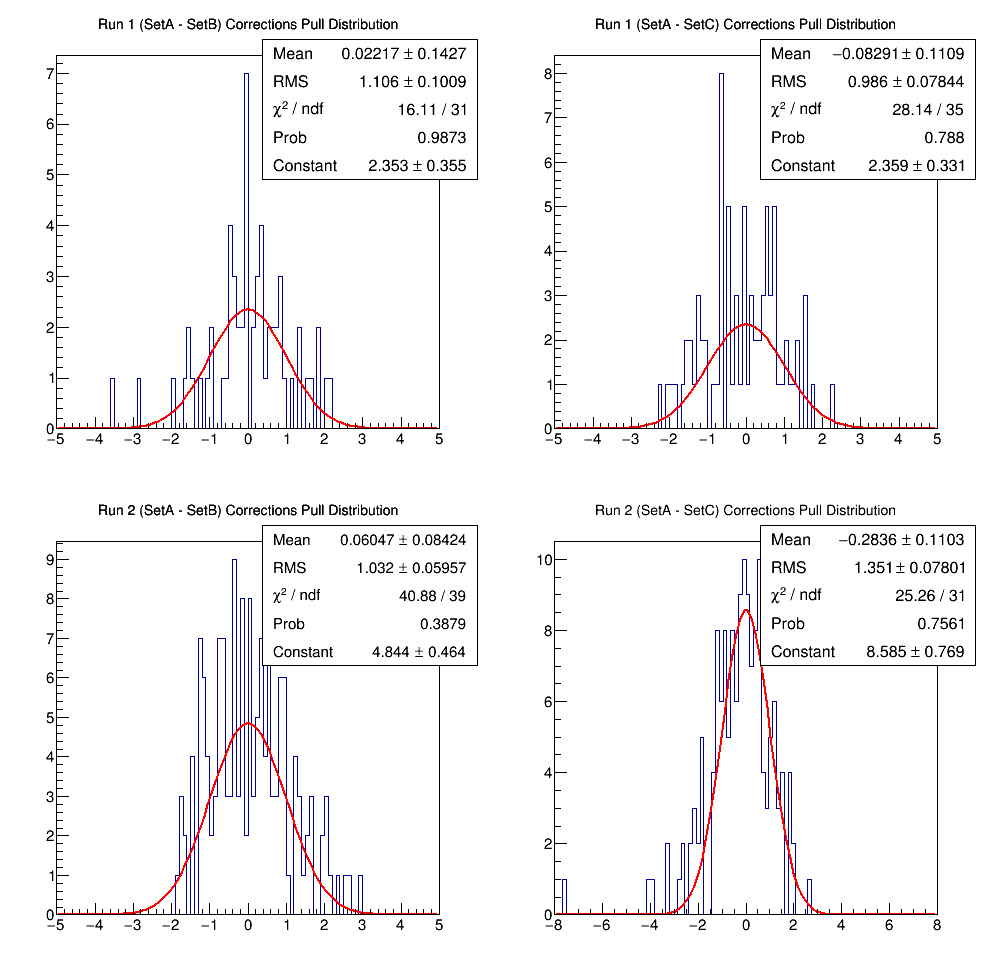
\includegraphics[width=5in]{Pictures/slug_pull_plots.png}}
\caption{Pull plot distributions for difference in corrections provided by monitor Set A and those of Sets B and C.  Each entry in the distributions is the average over a ``slug'' and represents about 8 hours of data. No sign-correction has been applied. The fit shown is for a Gaussian distribution with mean 0 and standard deviation 1 and with the scale factor as the only free parameter. At this averaging timescale, all monitor sets appear to give statistically consistent corrections. }
\label{fig:slug_pull_plots}
\end{figure}
 
A final test of the consistency can be made by comparing the fully corrected main detector averages using the three monitor sets. Once again the expected statistical variation between analyses can be estimated using the quadrature difference of the main detector average asymmetry error between analyses with different monitor sets. Table \ref{tab:physics_diff_mon_sets} shows the variation along with the expected statistical variation consistent with the asymmetry error change. Differences in the final physics asymmetries using the three monitor sets appear to be statistically consistent. 

\begin{table}[!h]
\caption{\label{tab:physics_diff_mon_sets}Comparison of average corrected physics asymmetries as given using the three different monitor sets. All values are in parts per billion (ppb). ``Statistical Difference'' refers to the quadrature difference between the asymmetry errors in the first two columns and is an estimate of the expected statistical variation consistent with the change in the asymmetry distribution width between two analyses. Asymmetry values shown for purposes of comparison and are not expected to precisely match those of the final \Qs dataset.  }
\begin{center}
\begin{tabular}[h]{|l|c|c|c|c|}\hline
~&Set A&Set B & Difference & Statistical \\ 
~&Asymmetry&Asymmetry&Set A - Set B&Difference\\ \hline
Run 1 & -218.2$\pm$12.7 & -220.1$\pm$12.9 & 1.9 &  $\pm$2.3 \\ \hline
Run 2 & -156.8$\pm$8.2  & -154.4$\pm$8.8&-2.4   & $\pm$3.2 \\ \hline
~&~&~&~&~\\
~&Set A&Set C & Difference & Statistical \\ 
~&Asymmetry&Asymmetry&Set A - Set C&Difference\\ \hline
Run 1 & -218.2$\pm$12.7 & -227.4$\pm$14.1 & 7.3 & $\pm$6.1\\ \hline
Run 2 & -156.8$\pm$8.2  & -159.2$\pm$9.7  & 4.8 & $\pm$5.2\\ \hline
\end{tabular}
\end{center}
\end{table}

The conclusion of this study is that short-timescale non-statistical differences between modulation analyses using different monitor set disappear over longer timescale averaging and are not apparent in the final corrected physics asymmetries. The most accurate results come from the default monitor set, Set A, which uses the target variables and BPM3c12X. 

\subsection{Long Timescale Detector to Monitor Sensitivity}
\label{sctn:residual_correlations}
The modulation analysis is meant to remove false asymmetries associated with helicity-correlated beam properties from the main detector data. The final corrected main detector data is expected to be uncorrelated with the monitors sensitive to those beam properties. However, noise such as electronics pickup, common to both the monitors and detectors will create false correlations that disappear with sufficient averaging. Therefore, one place to look for the success or failure of the modulation correction is in correlations between the main detector and beam monitors averaged over long timescales. Slug-level averaging was chosen for this correlation study where a ``slug'' is the amount of data taken on a specific HWP slow reversal state and is about 8 hours of data. Correlations of the main detector average (MDallbars) asymmetry were found by plotting the slug averages of the main detector versus the slug averages of the monitors over all Run 1 and Run 2. All asymmetries and monitor differences have been sign-corrected to remove the unwanted effects of the slow reversals. It is important to point out that this method is subject to false correlations arising from long-timescale changes in beam conditions. Long timescale drifts in charge or background asymmetries could create false long-timescale correlations. Since changes in beam conditions such as these are expected to be small, the residual correlations are a useful source of information; however, it is important to keep in mind that this method of determining residual correlations is intended only as a tool for finding large and well-determined residuals, not as a fine-resolution tool for distinguishing between plausible datasets. Tables \ref{tab:run1_residual_correlations_table} and  \ref{tab:run2_residual_correlations_table} show the residual correlations of the MDallbars asymmetry to the five monitors of interest to the modulation analysis as well as to the average current or charge measurement. A few schemes show large residual correlations to the beam monitors and can quickly be eliminated as unreliable. 

Fortunately, tables \ref{tab:run1_residual_correlations_table} and  \ref{tab:run2_residual_correlations_table} paint a rather unequivocal picture. Schemes that produce significant residual correlations to monitors are generally quite obvious with $>4\sigma$ significance and with more than one monitor showing large correlations. The residual charge correlation is not considered in this cutoff since it is not part of the modulation correction.  Cutting only the obviously problematic schemes eliminates the following schemes: ``Omit 0,3'', ``Omit 0,8'', ``Omit 3,5''\footnote{Scheme ``Omit 3,5'' has hints of residual correlations in Run 2 but the evidence for its removal is not conclusive. Choosing to remove or retain it does not change any of the arguments ahead.}, ``Omit 3,8'', ``Omit 5,8''\footnote{Scheme ``Omit 5,8'' is removed from Run 1 due to high residual correlations to monitors and from Run 2 because it does not contain sufficient information to find useful slopes for slugs 160-170 in Run 2.} and ``Omit 3''.  ``Omit 0'' must be removed from from Run 2 only, due to high residual correlations. Scheme ``Omit 1,4'' must also be eliminated from consideration for the entire dataset due the high level of instability in the correction slopes for this analysis. These eliminated schemes are shown as grayed out in tables \ref{tab:run1_dithering_corrections_table} - \ref{tab:run2_null_corrections_table}. 

It is tempting to try to further distinguish between modulation schemes using residual correlations as a measure of ``correctness''. For example, one might be tempted to choose the ``Omit 0,5'' scheme for Run 1 and the ``Omit 5'' scheme for Run 2 since the results of these alternate schemes appear to be better consistent with 0 correlations than the full 10-Coil scheme. As previously mentioned, these long-timescale residual correlations are not reliable as a fine-resolution tool for distinguishing the quality of schemes.

A case may be made for choosing the Omit 0,5 scheme based upon residual correlations to beam modulation and to the final corrected main detector width. When coils 0 and 5 are omitted from the analysis, the residual correlations for the other modulation coils are nearly consistent with 0 (see Figure \ref{fig:md_omit05_residuals}). This means that evidence for inconsistency between modulation coils is absent in this scheme. Although it could be argued that the number of X-type modulation coils has now been reduced to 3 which forces a 0 residual on the system, this argument does not stand up to scrutiny. This idea suggests that the system can be modeled by a block-diagonal matrix structure with essentially a $3\times3$ block with $X$, $X^{\prime}$ and $E$ mixing only with each other and a $2\times2$ block with $Y$ and $Y^{\prime}$ mixing. Thus using only 3 modulation coils for the X-type block forces the system of equations to have 0 residual sensitivity to X-type modulation coils. This is not the case. There is mixing between X-type and Y-type sensitivities meaning that X-type monitors are slightly sensitive to Y-type modulations and vice versa. Furthermore, not all schemes that remove two X-type coils successfully zero the residual sensitivities to the remaining X-type coils. So the argument for using the Omit 0,5 scheme is as follows: ``Inconsistency between modulation coils evidenced by residual correlations to the coils shows that there is a problem with one or more coils. This inconsistency mainly affects the X-type modulation and goes away for some schemes by removing two X-type coils. Using long timescale residual correlations of the main detector to beam monitors to further inform the choice of schemes leaves the Omit 0,5 as the only scheme with both residual correlations to monitors and residual sensitivity to modulation coils (when only the coils used in the analysis are considered) consistent with zero." 

Furthermore, the ``Omit 0,5'' scheme slightly reduces the corrected main detector asymmetry width beyond what the 10-Coil scheme does. Figure \ref{fig:md_width_compared} compares the width reduction of the MDallbars asymmetry distributions given by the two modulation schemes. The 10-Coil corrections increase the width of the MDallbars asymmetry for a large fraction of the \Qs dataset, whereas after slug 70 the Omit 0,5 corrections almost always reduce the width or leave it unchanged.
\begin{landscape}
\begin{table}[!h]

\caption{Run 1 residual correlations of MDallbars asymmetry to various beam monitors after dithering corrections. Blue colored correlations are $>3\sigma$ from 0 and Red are  $>4\sigma$.}
\begin{center}
\begin{tabular}[h]{|l|c|c|c|c|c|c|}\hline
Dithering&targetX&targetY&targetXSlope&targetYSlope&bpm3c12X&charge\\
~Scheme&(ppb/nm)&(ppb/nm)&(ppb/nrad)&(ppb/nrad)&(ppb/nm)&(ppb/ppb)\\\hline
10-Coil& +0.53$\pm$0.20& -0.65$\pm$0.30& +7.7$\pm$5.4& -10.9$\pm$6.4& +0.06$\pm$0.15& \color{red}+0.30$\pm$0.06\\\hline
Omit 0,3& \color{red}-1.07$\pm$0.20& \color{red}-2.55$\pm$0.30& \color{red}-48.7$\pm$5.4& \color{red}-60.2$\pm$6.4& \color{red}-1.30$\pm$0.15& \color{red}+0.27$\pm$0.06\\\hline
Omit 0,5& +0.31$\pm$0.20& -0.62$\pm$0.30& +5.8$\pm$5.4& -9.9$\pm$6.4& +0.15$\pm$0.15& \color{red}+0.29$\pm$0.06\\\hline
Omit 0,8& \color{blue}-0.61$\pm$0.20& \color{red}-1.25$\pm$0.30& \color{blue}-20.0$\pm$5.5& \color{red}-26.9$\pm$6.4& -0.43$\pm$0.15& \color{blue}+0.21$\pm$0.06\\\hline
Omit 3,5& -0.07$\pm$0.20& \color{red}-1.64$\pm$0.30& \color{blue}-17.4$\pm$5.4& \color{red}-34.9$\pm$6.4& \color{red}-0.68$\pm$0.15& \color{red}+0.30$\pm$0.06\\\hline
Omit 3,8& -0.55$\pm$0.20& \color{red}-2.27$\pm$0.30& \color{red}-39.1$\pm$5.4& \color{red}-52.2$\pm$6.4& \color{red}-1.41$\pm$0.15& \color{red}+0.27$\pm$0.06\\\hline
Omit 5,8& \color{red}+0.83$\pm$0.20& -0.32$\pm$0.30& \color{blue}+18.4$\pm$5.4& -2.7$\pm$6.4& +0.36$\pm$0.15& \color{red}+0.32$\pm$0.06\\\hline
Omit 1,4& -0.30$\pm$0.20& \color{red}-2.65$\pm$0.30& \color{red}-34.1$\pm$5.4& \color{red}-80.8$\pm$6.4& \color{red}-0.90$\pm$0.15& \color{red}+0.54$\pm$0.06\\\hline
Omit 1,6& \color{blue}+0.72$\pm$0.20& -0.54$\pm$0.30& +11.1$\pm$5.4& -9.1$\pm$6.4& +0.06$\pm$0.15& \color{red}+0.29$\pm$0.06\\\hline
Omit 1,9& +0.53$\pm$0.20& -0.64$\pm$0.30& +7.8$\pm$5.4& -10.7$\pm$6.4& +0.06$\pm$0.15& \color{red}+0.30$\pm$0.06\\\hline
Omit 4,6& +0.52$\pm$0.20& -0.59$\pm$0.30& +7.4$\pm$5.4& -9.8$\pm$6.4& +0.05$\pm$0.15& \color{red}+0.30$\pm$0.06\\\hline
Omit 4,9& +0.52$\pm$0.20& -0.69$\pm$0.30& +7.3$\pm$5.4& -11.8$\pm$6.4& +0.04$\pm$0.15& \color{red}+0.30$\pm$0.06\\\hline
Omit 6,9& \color{blue}+0.60$\pm$0.20& -0.29$\pm$0.30& +10.7$\pm$5.4& -2.9$\pm$6.4& +0.10$\pm$0.15& \color{red}+0.28$\pm$0.06\\\hline
Omit 2,7& \color{blue}+0.63$\pm$0.20& -0.67$\pm$0.30& +9.4$\pm$5.4& -11.5$\pm$6.4& +0.10$\pm$0.15& \color{red}+0.33$\pm$0.06\\\hline
Omit 0& -0.15$\pm$0.20& \color{blue}-0.95$\pm$0.30& -7.7$\pm$5.4& -18.9$\pm$6.4& -0.17$\pm$0.15& \color{red}+0.25$\pm$0.06\\\hline
Omit 1& +0.53$\pm$0.20& -0.64$\pm$0.30& +7.8$\pm$5.4& -10.7$\pm$6.4& +0.06$\pm$0.15& \color{red}+0.30$\pm$0.06\\\hline
Omit 2& +0.58$\pm$0.20& -0.66$\pm$0.30& +7.9$\pm$5.4& -11.1$\pm$6.4& +0.00$\pm$0.15& \color{red}+0.31$\pm$0.06\\\hline
Omit 3& -0.53$\pm$0.20& \color{red}-2.20$\pm$0.30& \color{red}-37.4$\pm$5.4& \color{red}-50.3$\pm$6.4& \color{red}-1.34$\pm$0.15& \color{red}+0.28$\pm$0.06\\\hline
Omit 4& +0.52$\pm$0.20& -0.67$\pm$0.30& +7.3$\pm$5.4& -11.5$\pm$6.4& +0.05$\pm$0.15& \color{red}+0.30$\pm$0.06\\\hline
Omit 5& \color{blue}+0.79$\pm$0.20& -0.38$\pm$0.30& \color{blue}+16.9$\pm$5.4& -4.0$\pm$6.4& +0.32$\pm$0.15& \color{red}+0.32$\pm$0.06\\\hline
Omit 6& +0.54$\pm$0.20& -0.62$\pm$0.30& +7.9$\pm$5.4& -10.3$\pm$6.4& +0.06$\pm$0.15& \color{red}+0.30$\pm$0.06\\\hline
Omit 7& +0.53$\pm$0.20& -0.65$\pm$0.30& +7.7$\pm$5.4& -10.8$\pm$6.4& +0.06$\pm$0.15& \color{red}+0.30$\pm$0.06\\\hline
Omit 8& +0.55$\pm$0.20& -0.62$\pm$0.30& +8.4$\pm$5.4& -10.2$\pm$6.4& +0.08$\pm$0.15& \color{red}+0.30$\pm$0.06\\\hline
Omit 9& +0.53$\pm$0.20& -0.65$\pm$0.30& +7.7$\pm$5.4& -10.9$\pm$6.4& +0.05$\pm$0.15& \color{red}+0.30$\pm$0.06\\\hline
\end{tabular}
\end{center}
\label{tab:run1_residual_correlations_table}
\end{table}

\begin{table}[!h]

\caption{Run 2 residual correlations of MDallbars asymmetry to various beam monitors after dithering corrections.}
\begin{center}
\begin{tabular}[h]{|l|c|c|c|c|c|c|}\hline
Dithering&targetX&targetY&tgtXSlope&tgtYSlope&bpm3c12X&charge\\
~Scheme&(ppb/nm)&(ppb/nm)&(ppb/nrad)&(ppb/nrad)&(ppb/nm)&(ppb/ppb)\\\hline
10-Coil& -0.14$\pm$0.14& -0.42$\pm$0.30& -4.6$\pm$5.5& -24$\pm$11& -0.00$\pm$0.29& +0.02$\pm$0.05\\\hline
Omit 0,3& \color{red}-1.00$\pm$0.17& \color{red}-2.72$\pm$0.45& \color{red}-37.7$\pm$6.1& \color{red}-93$\pm$15& \color{red}-1.83$\pm$0.34& -0.08$\pm$0.05\\\hline
Omit 0,5& -0.18$\pm$0.14& -0.47$\pm$0.30& -6.1$\pm$5.4& -26$\pm$11& -0.03$\pm$0.29& +0.02$\pm$0.05\\\hline
Omit 0,8& \color{red}-1.28$\pm$0.15& \color{red}-2.09$\pm$0.30& \color{red}-48.5$\pm$5.5& \color{red}-94$\pm$11& \color{red}-1.73$\pm$0.30& -0.10$\pm$0.05\\\hline
Omit 3,5& \color{blue}-0.45$\pm$0.14& -0.88$\pm$0.30& \color{blue}-16.9$\pm$5.5& \color{blue}-42$\pm$11& -0.50$\pm$0.30& -0.02$\pm$0.05\\\hline
Omit 3,8& \color{red}-1.00$\pm$0.15& \color{red}-1.70$\pm$0.30& \color{red}-38.3$\pm$5.5& \color{red}-75$\pm$11& \color{red}-1.37$\pm$0.30& -0.08$\pm$0.05\\\hline
Omit 5,8& +0.24$\pm$0.17& +0.42$\pm$0.44& +9.1$\pm$6.0& -2$\pm$14& +0.33$\pm$0.34& +0.08$\pm$0.05\\\hline
Omit 1,4& -0.18$\pm$0.15& -0.54$\pm$0.30& -5.2$\pm$5.5& \color{blue}-38$\pm$11& +0.05$\pm$0.30& +0.04$\pm$0.05\\\hline
Omit 1,6& -0.13$\pm$0.14& -0.42$\pm$0.30& -4.4$\pm$5.5& -23$\pm$11& +0.02$\pm$0.29& +0.02$\pm$0.05\\\hline
Omit 1,9& -0.14$\pm$0.14& -0.42$\pm$0.30& -4.6$\pm$5.5& -24$\pm$11& -0.00$\pm$0.29& +0.03$\pm$0.05\\\hline
Omit 4,6& -0.14$\pm$0.14& -0.44$\pm$0.30& -4.7$\pm$5.5& -24$\pm$11& +0.00$\pm$0.29& +0.02$\pm$0.05\\\hline
Omit 4,9& -0.15$\pm$0.14& -0.44$\pm$0.30& -4.8$\pm$5.5& -24$\pm$11& -0.01$\pm$0.29& +0.02$\pm$0.05\\\hline
Omit 6,9& -0.11$\pm$0.14& -0.36$\pm$0.30& -3.4$\pm$5.5& -21$\pm$11& +0.05$\pm$0.29& +0.02$\pm$0.05\\\hline
Omit 2,7& -0.05$\pm$0.14& -0.17$\pm$0.30& -1.6$\pm$5.5& -14$\pm$11& +0.04$\pm$0.30& +0.02$\pm$0.05\\\hline
Omit 0& \color{red}-0.71$\pm$0.14& \color{red}-1.26$\pm$0.30& \color{red}-26.7$\pm$5.5& \color{red}-59$\pm$11& -0.88$\pm$0.29& -0.04$\pm$0.05\\\hline
Omit 1& -0.14$\pm$0.14& -0.43$\pm$0.30& -4.7$\pm$5.5& -24$\pm$11& -0.01$\pm$0.29& +0.02$\pm$0.05\\\hline
Omit 2& -0.12$\pm$0.14& -0.38$\pm$0.30& -3.7$\pm$5.5& -22$\pm$11& +0.13$\pm$0.30& +0.02$\pm$0.05\\\hline
Omit 3& \color{red}-0.90$\pm$0.15& \color{red}-1.55$\pm$0.30& \color{red}-34.7$\pm$5.5& \color{red}-69$\pm$11& \color{red}-1.24$\pm$0.30& -0.07$\pm$0.05\\\hline
Omit 4& -0.14$\pm$0.14& -0.43$\pm$0.30& -4.7$\pm$5.5& -24$\pm$11& -0.00$\pm$0.29& +0.02$\pm$0.05\\\hline
Omit 5& +0.05$\pm$0.14& -0.13$\pm$0.30& +3.0$\pm$5.5& -12$\pm$11& +0.31$\pm$0.29& +0.05$\pm$0.05\\\hline
Omit 6& -0.14$\pm$0.14& -0.42$\pm$0.30& -4.5$\pm$5.5& -23$\pm$11& +0.01$\pm$0.29& +0.02$\pm$0.05\\\hline
Omit 7& -0.14$\pm$0.14& -0.42$\pm$0.30& -4.6$\pm$5.5& -24$\pm$11& -0.00$\pm$0.29& +0.02$\pm$0.05\\\hline
Omit 8& -0.13$\pm$0.14& -0.42$\pm$0.30& -4.2$\pm$5.5& -23$\pm$11& +0.03$\pm$0.29& +0.03$\pm$0.05\\\hline
Omit 9& -0.15$\pm$0.14& -0.43$\pm$0.30& -4.8$\pm$5.5& -24$\pm$11& -0.01$\pm$0.29& +0.02$\pm$0.05\\\hline
\end{tabular}
\end{center}
\label{tab:run2_residual_correlations_table}
\end{table}
\begin{figure}[ht]
%~/thesis_plot_macros/omit05_residuals_vs_slug.C
\centering
\framebox{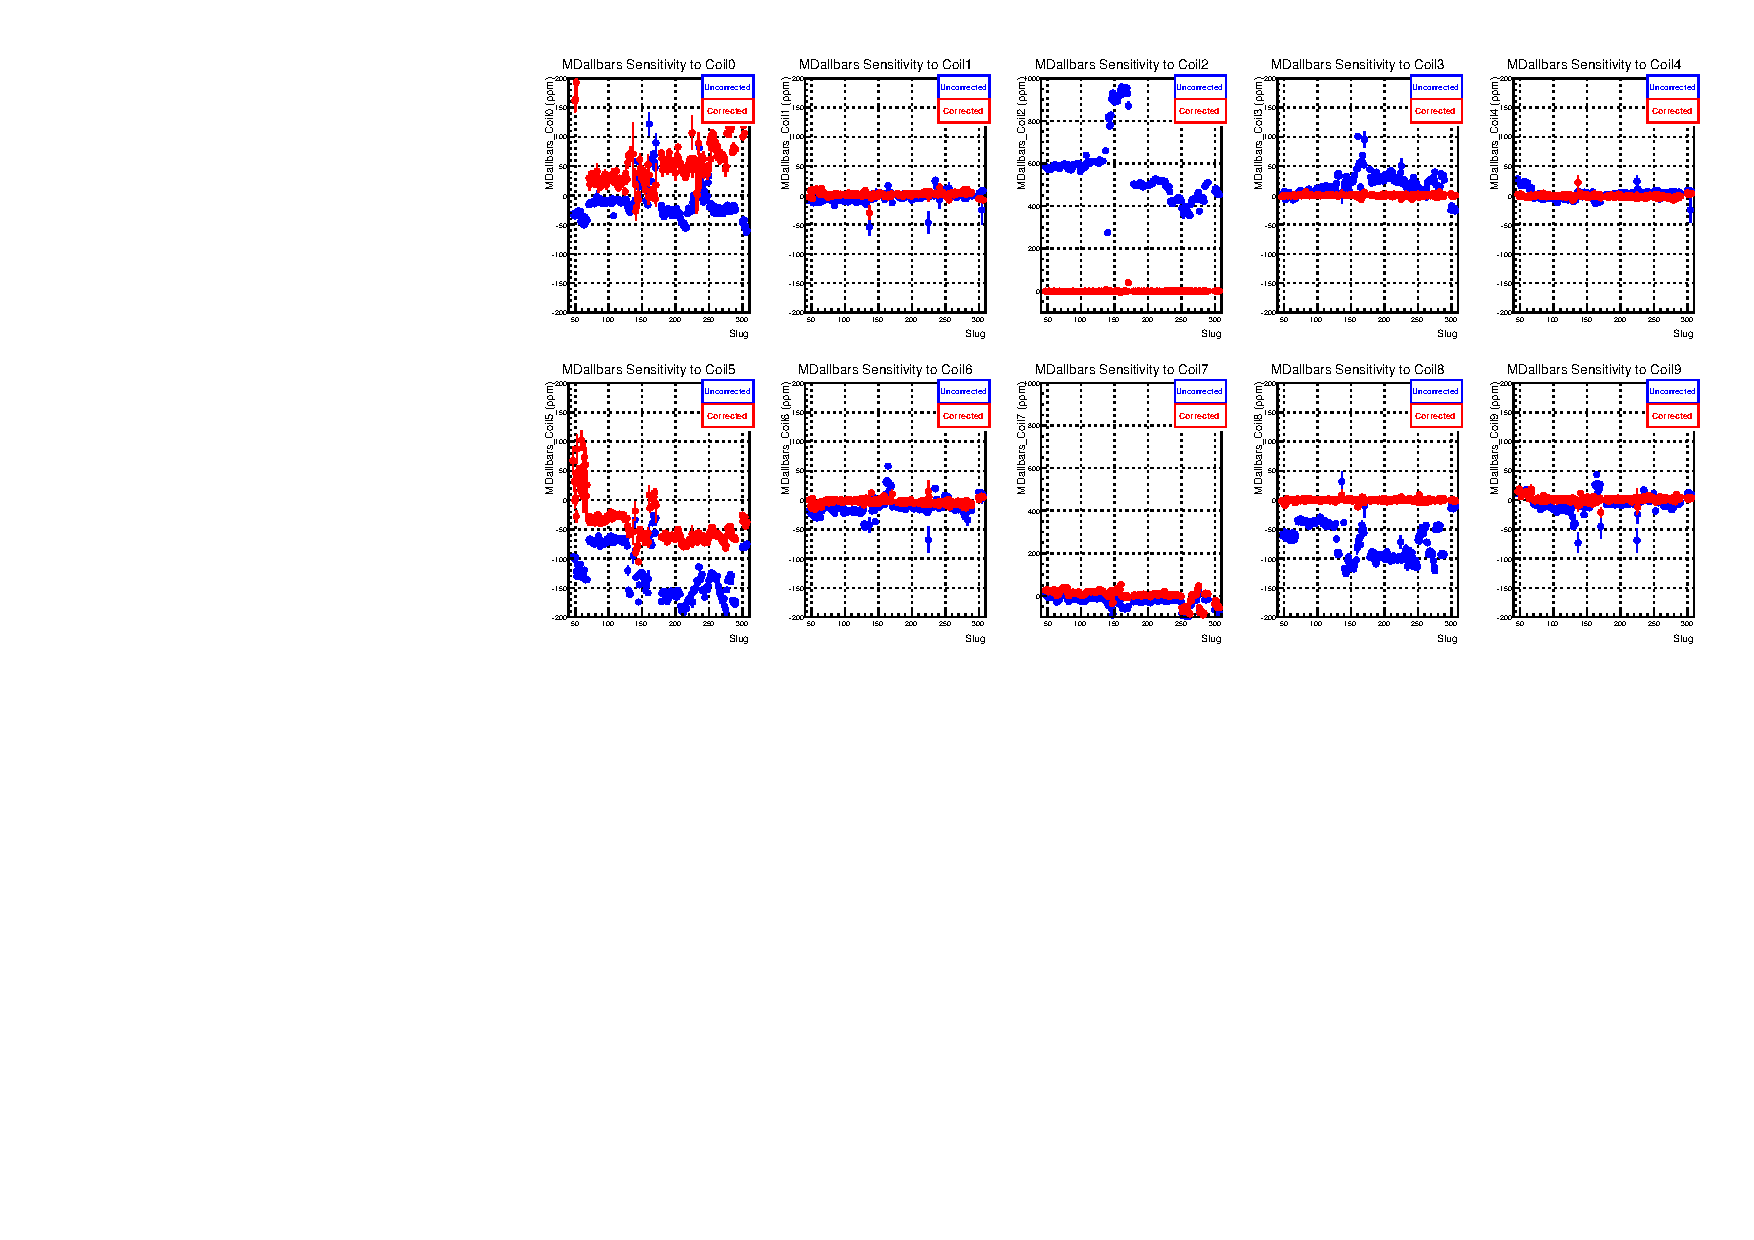
\includegraphics[width=8.9in]{Pictures/omit05_residuals.pdf}}
\caption{Residual sensitivity of MDallbars to modulation coils for modulation scheme omitting coils 0 and 5 (``Omit 0,5'' scheme) from the analysis. The residual sensitivities remain large to  coils 0 and 5 as expected, but go to nearly 0 for the other X-type coils 3 and 8. Sensitivities to Y-type coils are small before correction and remain small after correction}
\label{fig:md_omit05_residuals}
\end{figure}
\end{landscape}

\begin{figure}[ht]

\centering
\framebox{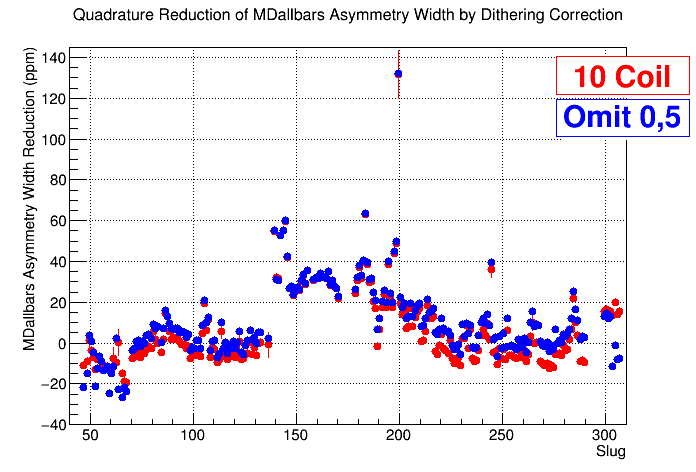
\includegraphics[width=5in]{Pictures/MD_width_compared.png}}
\caption{Shown is the width reduction of MDallbars asymmetry quartet distribution for ``10-Coil'' and ``Omit 0,5'' schemes. Width reduction is calculated as the quadrature difference of the width of the uncorrected and modulation corrected MDallbars asymmetry distributions. The sign of the quadrature difference is assigned such that negative numbers means the modulation correction increased the width.}
\label{fig:md_width_compared}
\end{figure}

Having established at least a plausible argument for using the ``Omit 0,5'' corrections perhaps it would be prudent to look at variations around the ``Omit 0,5'' results that occur from omitting various Y-like coils in addition to coils 0 and 5. 

Tables \ref{tab:run1_om05_residual_correlations_table} and \ref{tab:run2_om05_residual_correlations_table} show the residual correlations for various Y-type coil omissions paired with omitting coils 0 and 5. The only elimination that can be made at the $3\sigma$ level is the scheme that omits coils 0, 1, 4 and 5 (``Omit 0,5,1,4'') and that only during Run 1. The last row of these tables shows an example of a five coil analysis where Coil 7 (out-of-phase energy modulation) is also omitted in addition to two X-type and two Y-type coils, which produces zero-residuals in the five coils used by definition. No further distinction can be made between the remaining schemes using these residual correlations. 


\begin{table}[!h]
\caption{Run 1 residual correlations of MDallbars asymmetry to various beam monitors after dithering corrections using various coil selections. Blue-colored cells have residual correlations with $3\sigma$ significance and  red-colored cells have residual correlations with $4\sigma$ significance.}
\begin{center}
\begin{tabular}[h]{|l|c|c|c|c|c|}\hline
Dithering&targetX&targetY&targetXSlope&targetYSlope&bpm3c12X\\
~Scheme&(ppb/nm)&(ppb/nm)&(ppb/nrad)&(ppb/nrad)&(ppb/nm)\\\hline
Omit0,5& 0.31$\pm$0.20& -0.62$\pm$0.30& 5.9$\pm$5.4& -9.9$\pm$6.4& 0.15$\pm$0.15\\\hline
Omit0,5,1,4&\color{blue} 0.60$\pm$0.20& 0.18$\pm$0.29& \color{red}21.5$\pm$5.4&\color{blue} 20.7$\pm$6.4& 0.37$\pm$0.15\\\hline
Omit0,5,1,6& 0.15$\pm$0.20& -0.66$\pm$0.30& 3.5$\pm$5.4& -10.3$\pm$6.4& 0.18$\pm$0.15\\\hline
Omit0,5,1,9& 0.30$\pm$0.20& -0.63$\pm$0.30& 5.9$\pm$5.4& -9.8$\pm$6.4& 0.15$\pm$0.15\\\hline
Omit0,5,4,6& 0.31$\pm$0.20& -0.59$\pm$0.30& 5.7$\pm$5.4& -9.4$\pm$6.4& 0.14$\pm$0.15\\\hline
Omit0,5,4,9& 0.29$\pm$0.20& -0.67$\pm$0.30& 5.3$\pm$5.4& -11.1$\pm$6.4& 0.14$\pm$0.15\\\hline
Omit0,5,6,9& 0.27$\pm$0.20& -0.54$\pm$0.30& 5.1$\pm$5.4& -8.7$\pm$6.4& 0.12$\pm$0.15\\\hline
Omit0,5,6,7,9& 0.26$\pm$0.20& -0.55$\pm$0.30& 5.0$\pm$5.4& -8.8$\pm$6.4& 0.12$\pm$0.15\\\hline
\end{tabular}
\end{center}
\label{tab:run1_om05_residual_correlations_table}
\end{table}
\begin{table}[!h]
\caption{Run 2 residual correlations of MDallbars asymmetry to various beam monitors after dithering corrections using various coil selections.}
\begin{center}
\begin{tabular}[h]{|l|c|c|c|c|c|}\hline
Dithering&targetX&targetY&targetXSlope&targetYSlope&bpm3c12X\\
~Scheme&(ppb/nm)&(ppb/nm)&(ppb/nrad)&(ppb/nrad)&(ppb/nm)\\\hline
Omit0,5& -0.18$\pm$0.14& -0.47$\pm$0.30& -6.1$\pm$5.5& -26$\pm$11& -0.03$\pm$0.29\\\hline
Omit0,5,1,4& -0.16$\pm$0.14& -0.42$\pm$0.30& -5.4$\pm$5.5& -23$\pm$11& -0.01$\pm$0.30\\\hline
Omit0,5,1,6& -0.19$\pm$0.14& -0.50$\pm$0.30& -6.4$\pm$5.5& -27$\pm$11& -0.04$\pm$0.29\\\hline
Omit0,5,1,9& -0.18$\pm$0.14& -0.48$\pm$0.30& -6.1$\pm$5.5& -26$\pm$11& -0.04$\pm$0.29\\\hline
Omit0,5,4,6& -0.19$\pm$0.14& -0.50$\pm$0.30& -6.5$\pm$5.5& -27$\pm$11& -0.04$\pm$0.29\\\hline
Omit0,5,4,9& -0.19$\pm$0.14& -0.48$\pm$0.30& -6.2$\pm$5.5& -26$\pm$11& -0.04$\pm$0.29\\\hline
Omit0,5,6,9& -0.19$\pm$0.14& -0.49$\pm$0.30& -6.5$\pm$5.5& -26$\pm$11& -0.05$\pm$0.29\\\hline
Omit0,5,6,7,9& -0.19$\pm$0.14& -0.48$\pm$0.30& -6.4$\pm$5.5& -26$\pm$11& -0.05$\pm$0.29\\\hline
\end{tabular}
\end{center}
\label{tab:run2_om05_residual_correlations_table}
\end{table}

Tables \ref{tab:run1_dithering_corrections_table} and \ref{tab:run2_dithering_corrections_table} show that omitting various combinations Y-type coils (1, 4, 6, and 9) while using all X-type coils creates a spread of total corrections around the 10-Coil values. For Run 1 the 10-Coil correction is -19.2~ppb. The values for omitting various Y coils are approximately centered on this value with a range of -16.7~ppb to  22.0~ppb. For Run 2 there is a similar spread centered on the 10-Coil correction of -1.7~ppb with a range from -1.5~ppb to -1.8~ppb from analyses omitting different combinations of Y-type coils. A similar analysis ``centered on'' the ``Omit 0,5'' scheme reveals a similar spread. Tables \ref{tab:run1_om05_dithering_corrections} and \ref{tab:run2_om05_dithering_corrections} show similar results for omitting Y-coils in addition to omitting coils 0 and 5. For Run 1 the total correction for ``Omit 0,5'' is -13.6~ppb with a range from -12.4~ppb to -16.1~ppb for schemes with additional Y-coil omissions. Similarly for Run 2 the ``Omit 0,5'' correction is -2.4~ppb with a range from -2.1~ppb to -2.6~ppb for schemes with further Y-coil omissions.
\begin{table}[!h]

\caption{\label{tab:run1_om05_dithering_corrections}Run 1 dithering corrections for MDallbars asymmetry compared for different coil selections. ``Omit0,5,1,4'' results grayed out due to large residual correlations seen in Table \ref{tab:run1_om05_residual_correlations_table}}
\begin{center}
\begin{tabular}[h]{|l||c|c|c|c|c||c|}\hline
Dithering& Wien 1& Wien 2& Wien 3& Wien 4& Wien 5& Total\\
~Scheme&(ppb)&(ppb)&(ppb)&(ppb)&(ppb)&(ppb)\\\hline\hline
Omit0,5& -19.2& +21.6& -43.9& -16.9& -14.9& -13.6\\\hline
{\color{Gray}Omit0,5,1,4}&{\color{Gray} -30.6}&{\color{Gray} +35.1}&{\color{Gray} -36.9}&{\color{Gray} +46.2}&{\color{Gray} -8.9}&{\color{Gray} +3.4}\\\hline
Omit0,5,1,6& -17.9& +26.1& -45.1& -16.3& -14.7& -12.4\\\hline
Omit0,5,1,9& -19.2& +20.2& -45.1& -17.5& -15.2& -14.3\\\hline
Omit0,5,4,6& -35.5& +22.0& -45.2& -15.8& -15.7& -16.1\\\hline
Omit0,5,4,9& -13.4& +18.8& -45.2& -17.6& -16.1& -14.0\\\hline
Omit0,5,6,9& -19.2& +20.6& -44.8& -14.5& -15.1& -13.6\\\hline
Omit0,5,6,7,9& -19.2& +20.3& -44.6& -14.4& -15.4& -13.6\\\hline
\end{tabular}
\end{center}
\end{table}
\begin{table}[!h]

\caption{\label{tab:run2_om05_dithering_corrections}Run 2 dithering corrections for MDallbars asymmetry compared for different coil selections.}
\begin{center}
\begin{tabular}[h]{|l||c|c|c|c|c|c||c|}\hline
Dithering& Wien 6& Wien 7& Wien 8a& Wien 8b& Wien 9a& Wien 9b& Total\\
~Scheme&(ppb)&(ppb)&(ppb)&(ppb)&(ppb)&(ppb)&(ppb)\\\hline\hline
Omit0,5& -24.7& +36.0& -13.9& -5.3& +1.7& +0.2& -2.4\\\hline
Omit0,5,1,4& -31.3& +31.6& -11.8& -1.1& +2.1& +0.9& -2.1\\\hline
Omit0,5,1,6& -24.5& +38.2& -13.9& -4.7& +0.8& +0.2& -2.3\\\hline
Omit0,5,1,9& -24.4& +35.9& -13.9& -4.7& +0.9& +0.1& -2.5\\\hline
Omit0,5,4,6& -24.4& +38.1& -14.1& -4.7& +0.7& +0.3& -2.4\\\hline
Omit0,5,4,9& -24.2& +36.0& -14.3& -5.0& +0.8& +0.2& -2.6\\\hline
Omit0,5,6,9& -24.9& +36.6& -13.8& -4.7& +0.8& +0.3& -2.5\\\hline
Omit0,5,6,7,9& -24.9& +36.7& -13.8& -4.6& +0.7& +0.3& -2.4\\\hline
\end{tabular}
\end{center}
\end{table}

Thus it appears that there are two clusters of modulation results-- a cluster formed by various Y-coil omissions centered on the 10-Coil result and a cluster formed by various Y-coil omissions centered on the ``Omit 0,5'' result. The ``10-Coil'' and ``Omit 0,5'' results are good representatives of these two clusters both of which produce MDallbars results with residual correlations to beam monitors that are consistent with zero. 

\subsection{Signature of the Inconsistency}
Before attempting to determine a final modulation correction and assign a systematic error it is important to look at a key feature of the failure or inconsistency of the modulation analysis. Considering the azimuthal arrangement of the main detector bars (see Figure \ref{fig:octant_coords}) allows one to qualitatively predict responses of individual bars. For example, the response of bar 1 should be equal and opposite of that of bar 5 to horizontal position and angle modulation, whereas bars 3 and 7 should see small but equal responses to horizontal modulations. The response of the main detector to position or angle modulation as a function of the octant angle around the azimuth should have an approximately sinusoidal pattern. These sinusoidal patterns are referred to as ``dipoles'' and in the jargon of \Qs when the maximum response is in the vertical direction (maximum response on bars 3 and 7) it is referred to  as a ``vertical dipole''. Likewise when the maximum response is in the horizontal direction (maximum response on bars 1 and 5), it is called a ``horizontal dipole''. Thus, X-type modulations will create horizontal dipole responses and Y-type modulations are expected to produce vertical dipole responses. Any effect that creates equal responses in all detector bars is called a ``monopole response''. Shifts in energy and charge are candidates for monopole responses. Examples of dipole and monopole responses to the various types of X and Y modulations before and after correction  can be seen in figures \ref{fig:Run2_10coil_Xdipoles} and \ref{fig:Run2_10coil_Ydipoles}. The dipole response is given by the amplitude of the sinusoid, while the monopole is the offset. While a more detailed analysis of the main detector dipole and monopole response patterns is investigated in Appendix \ref{AppendixD}, the most significant observations are as follows:\\
1. The failure mode of the beam modulation analysis affects all the main detectors equally. A monopole residual sensitivity is evident whereas the dipoles are removed.\\
2. The successful removal of dipoles is a feature of even of coil schemes deemed untrustworthy due to large residual correlations to monitors they produce. Expected geometric sensitivities are removed but failure to remove the source of monopole sensitivity is evident for all schemes, although not equally.\\
3. The residual monopole responses are largest for the X-coils. Omitting coils 0 and 5 shrinks the monopole responses in the other two X-coils (3 and 8) to be consistent with zero while enlarging the monopole response in the omitted coils (coils 0 and 5). However, even for coils omitted from the analysis, the residual dipole response is consistent with zero.\\ 

It is tempting to consider the energy correction as a possible source of this monopole residual, since the energy response in a detector system with perfect azimuthal symmetry would be monopole. However, the evidence against this hypothesis is threefold. First, in the analysis where beam monitors were corrected using the same modulation analysis toolset, energy sensitive BPM's did not show residual sensitivities. Second, the \qtor spectrometer and detector system do not manifest perfect azimuthal symmetry. The combination of mean beam position and angle, differences in the magnetic field from octant to octant in the spectrometer, as well as small errors in the positioning of the detectors, conspire to create an energy response that is far from monopole in the main detector. The characteristic response pattern of the main detector to energy modulation is seen in Figure \ref{fig:Run2_10coil_Edipole}. Third, changing the BPM used in the modulation analysis from one in a horizontally dispersive region to one with less sensitivity and in a vertically dispersive region showed no evidence of statistically different corrections averaged over slug timescales or over the entire dataset.

\begin{figure}[!ht]
\begin{center}
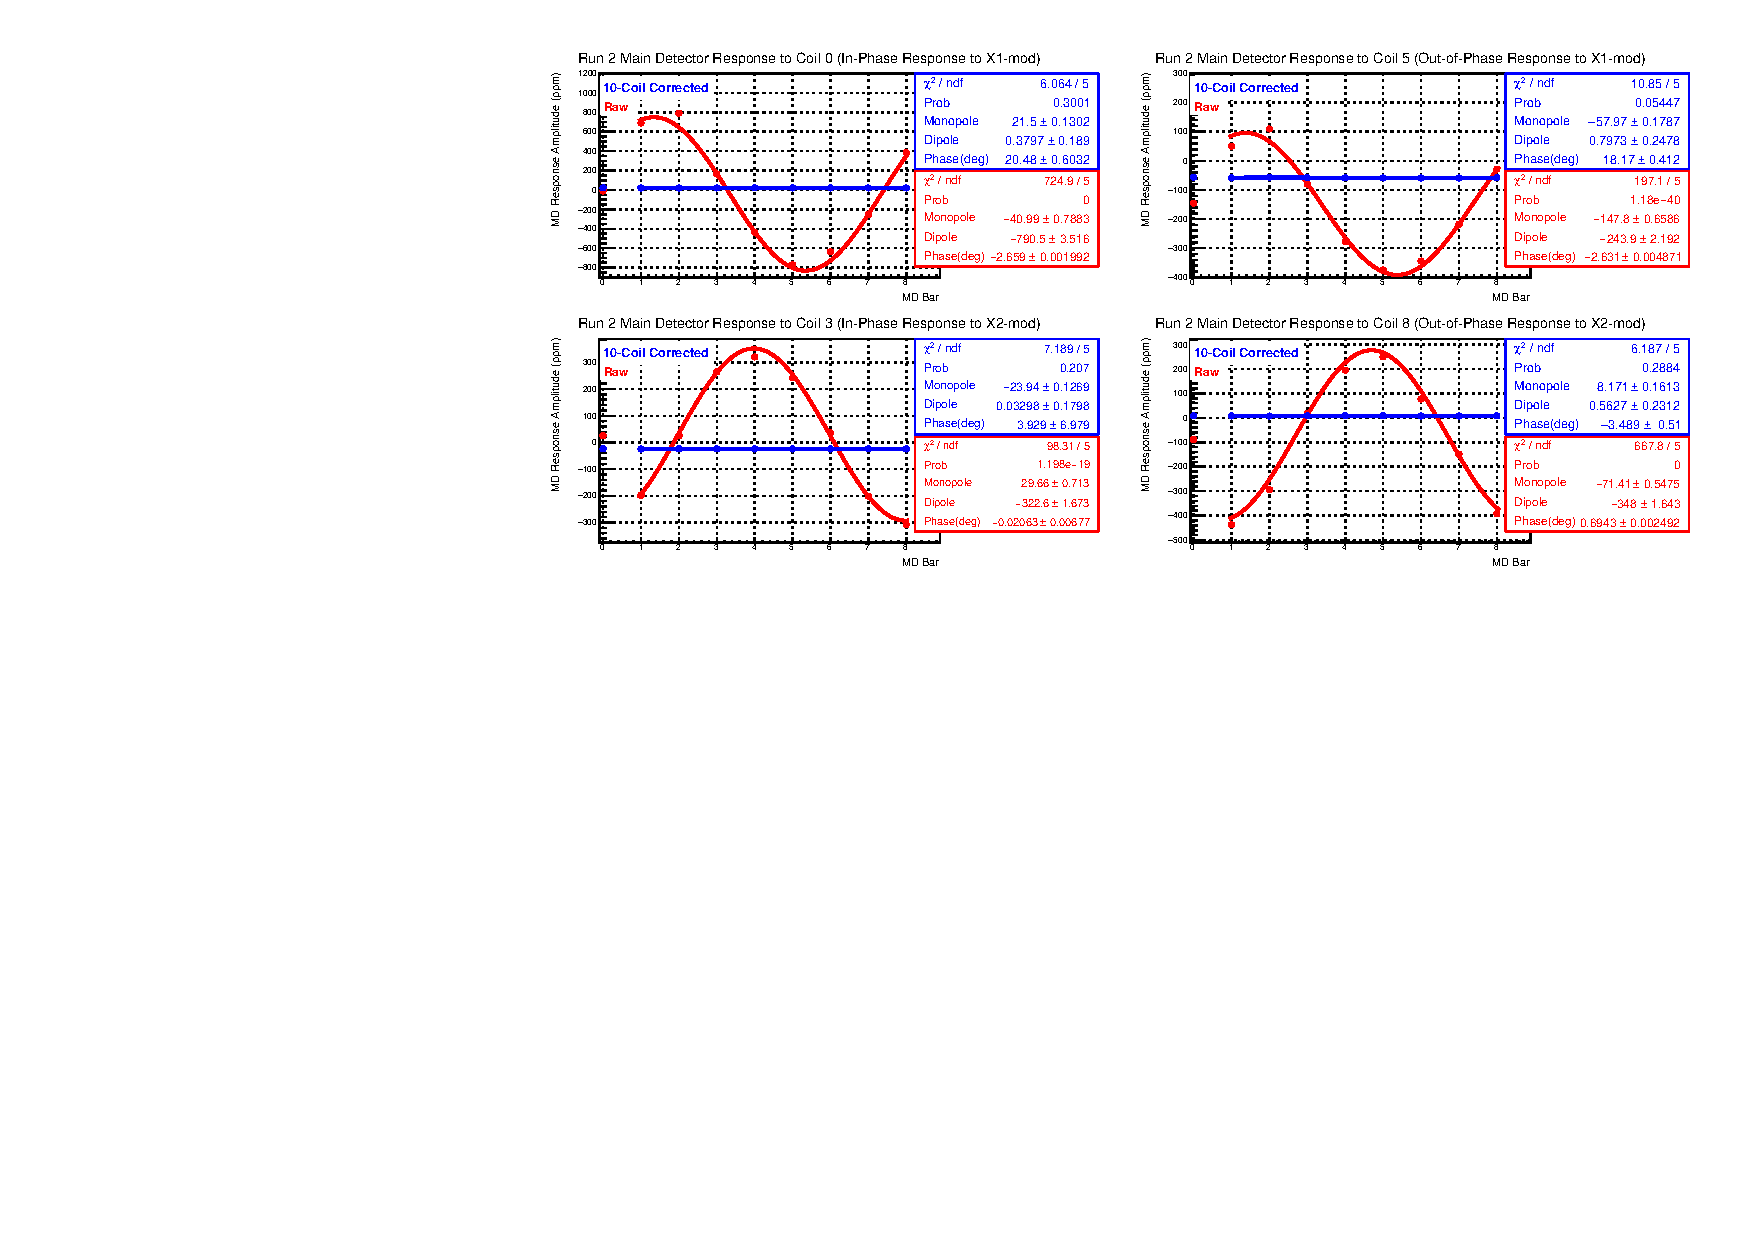
\includegraphics[width=5.9in]{./Pictures/Run2_X_dipole10-Coil.pdf}
\caption{\label{fig:Run2_10coil_Xdipoles}Responses of individual main detector bars averaged over Run 2 to X-type modulation coils before correction and after correction using a full 10-Coil analysis. The dipole response is given by the amplitude of the sinusoid while the monopole is the offset. The response of MDallbars is given by the point at Bar 0.}
\end{center}
\end{figure}
\begin{figure}[!ht]
\begin{center}
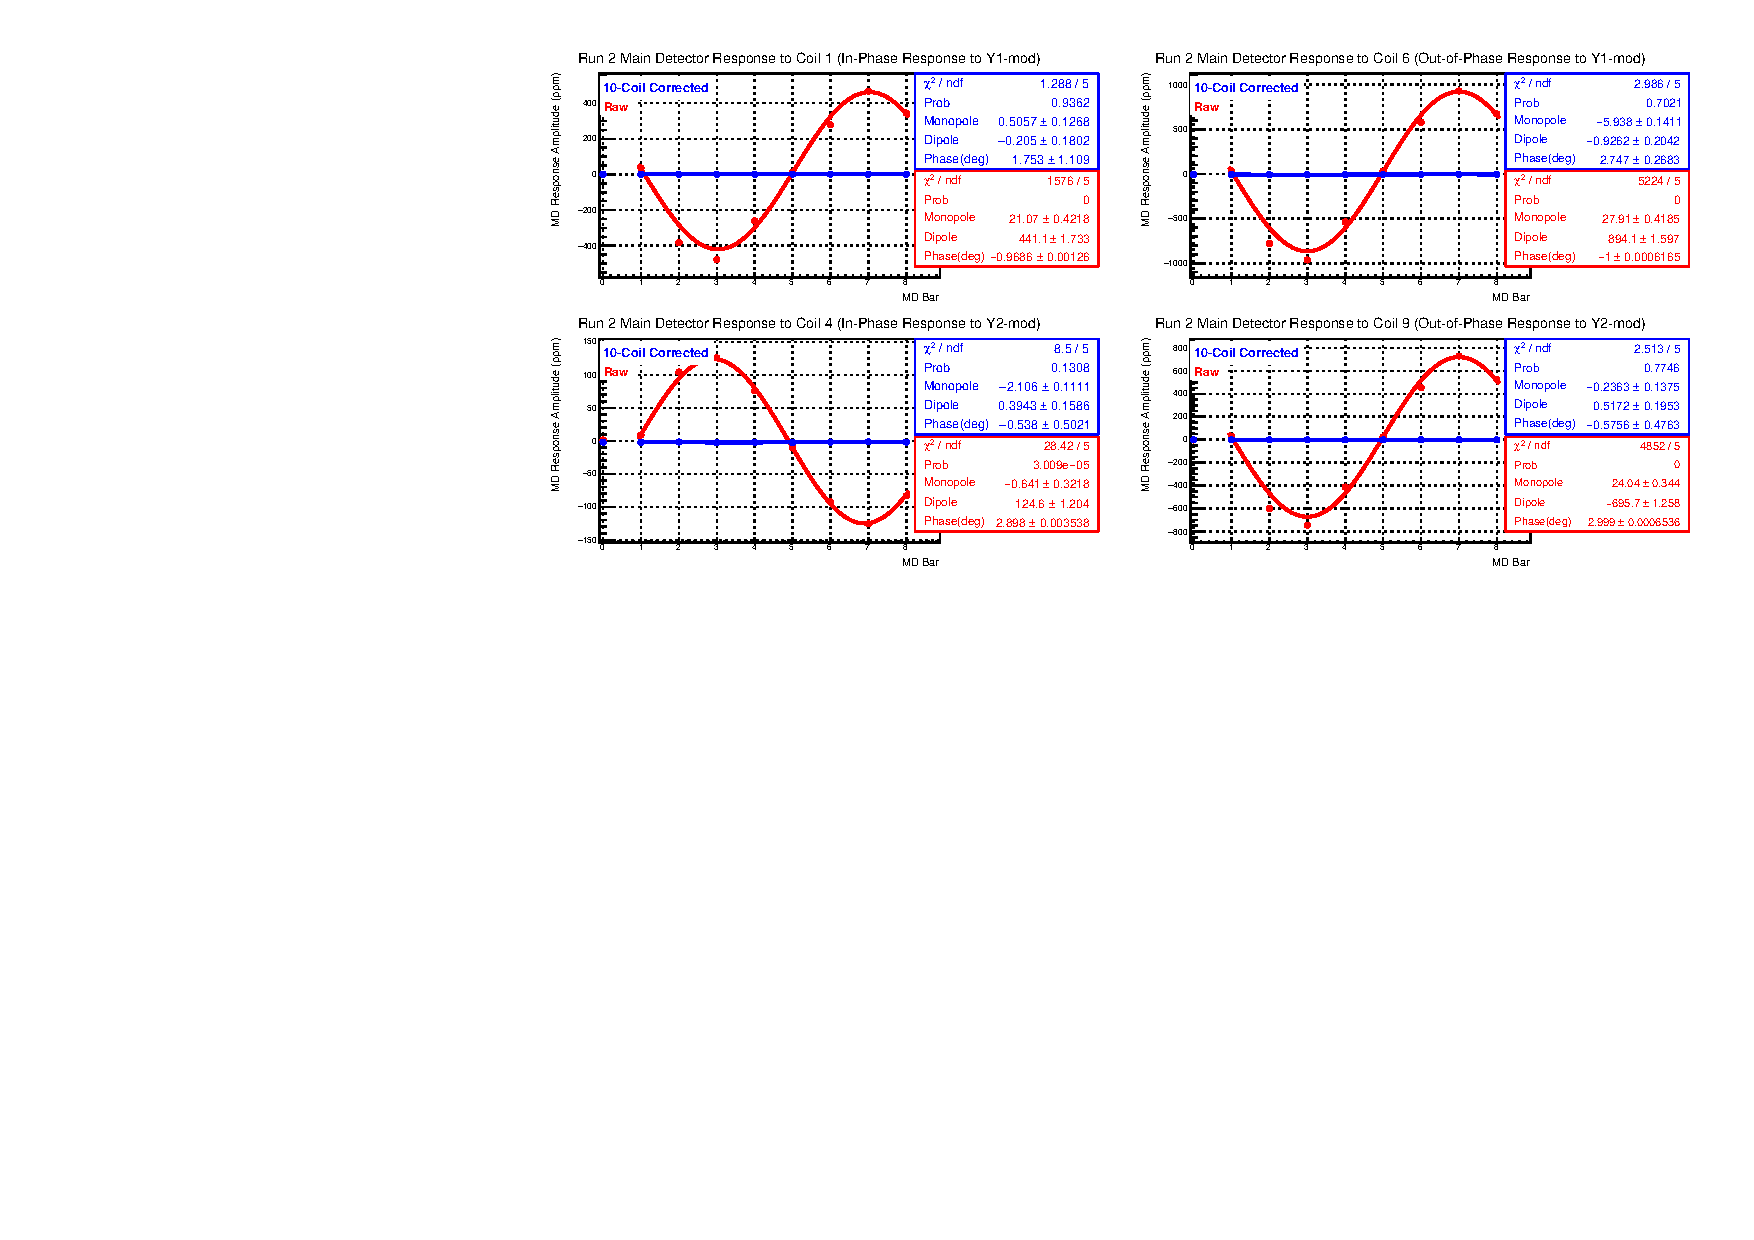
\includegraphics[width=5.9in]{./Pictures/Run2_Y_dipole10-Coil.pdf}
\caption{\label{fig:Run2_10coil_Ydipoles}Responses of individual main detector bars averaged over Run 2 to Y-type modulation coils before correction and after correction using a full 10-Coil analysis. The dipole response is given by the amplitude of the sinusoid while the monopole is the offset. The response of MDallbars is given by the point at Bar 0.}
\end{center}
\end{figure}

\begin{figure}[!ht]
\begin{center}
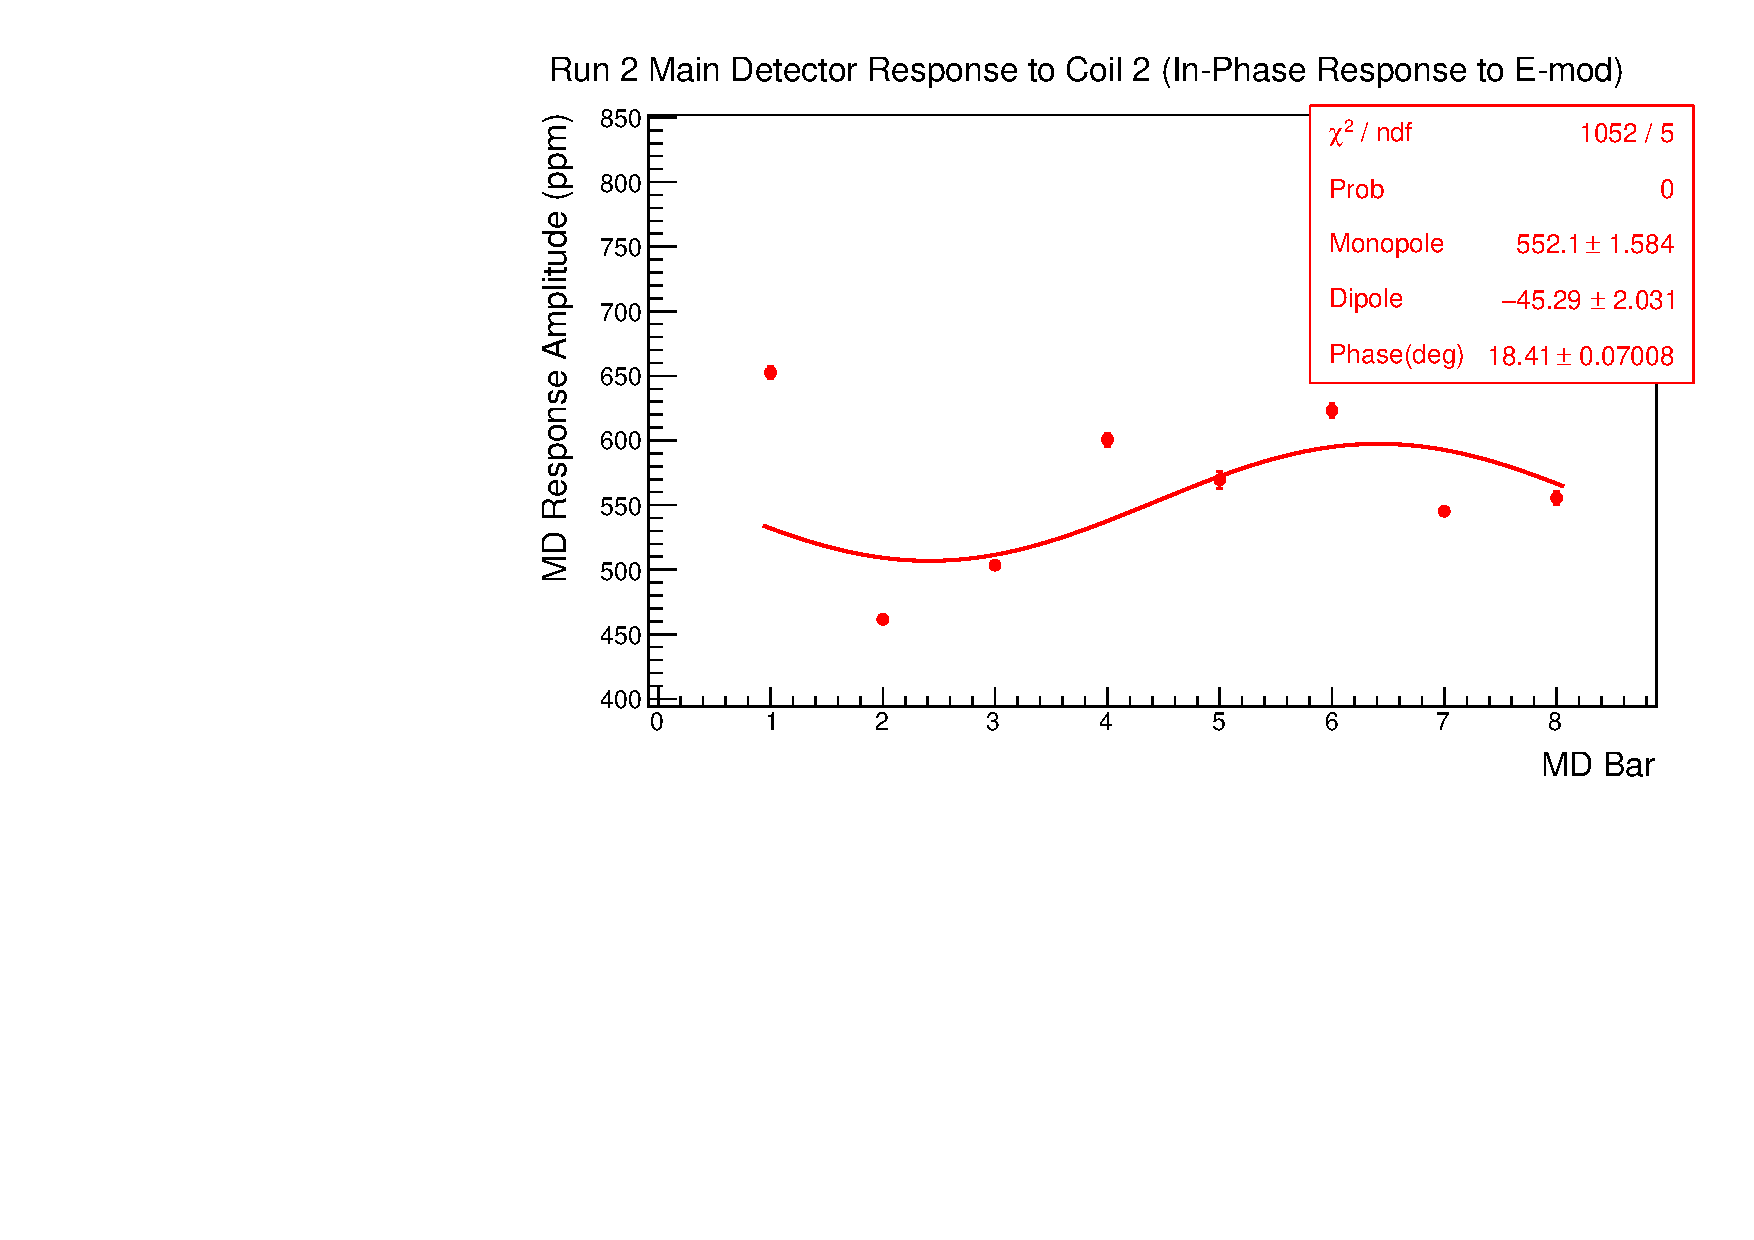
\includegraphics[width=4in]{./Pictures/Run2_E-response_10coil.pdf}
\caption{\label{fig:Run2_10coil_Edipole}Responses of individual main detector bars averaged over Run 2 to energy modulation. Although dipole and monopole values are shown, the shape is not well characterized by either and instead gets its characteristic pattern from broken azimuthal symmetry in the electron beam/spectrometer/detector system.}
\end{center}
\end{figure}

A final potential failure mode that needs to be ruled out as a candidate for producing the monopole residual responses is charge or current. Although all detectors are normalized to the charge and are not expected to be sensitive to charge fluctuations to first order, there are subtle ways in which charge could still create monopole residuals. Imagine, for example, the BCM(s) used for charge normalization somehow picking up the modulation signal. This would not be visible on the battery or source channels previously monitored since they are not normalized to charge. To test the ``monopole residuals from charge'' hypothesis, a full analysis was done using main detector signals that were not normalized to charge. Figure \ref{fig:no_Q_norm_slopes}  compares the correction slopes found using normalized and unnormalized detectors and although small shifts are evident, these do not remove the residual sensitivities to modulation coils (see Figure \ref{fig:no_Q_norm_residuals}). Apparently charge is not the culprit either.
\begin{landscape}
\begin{figure}[!ht]
\begin{center}
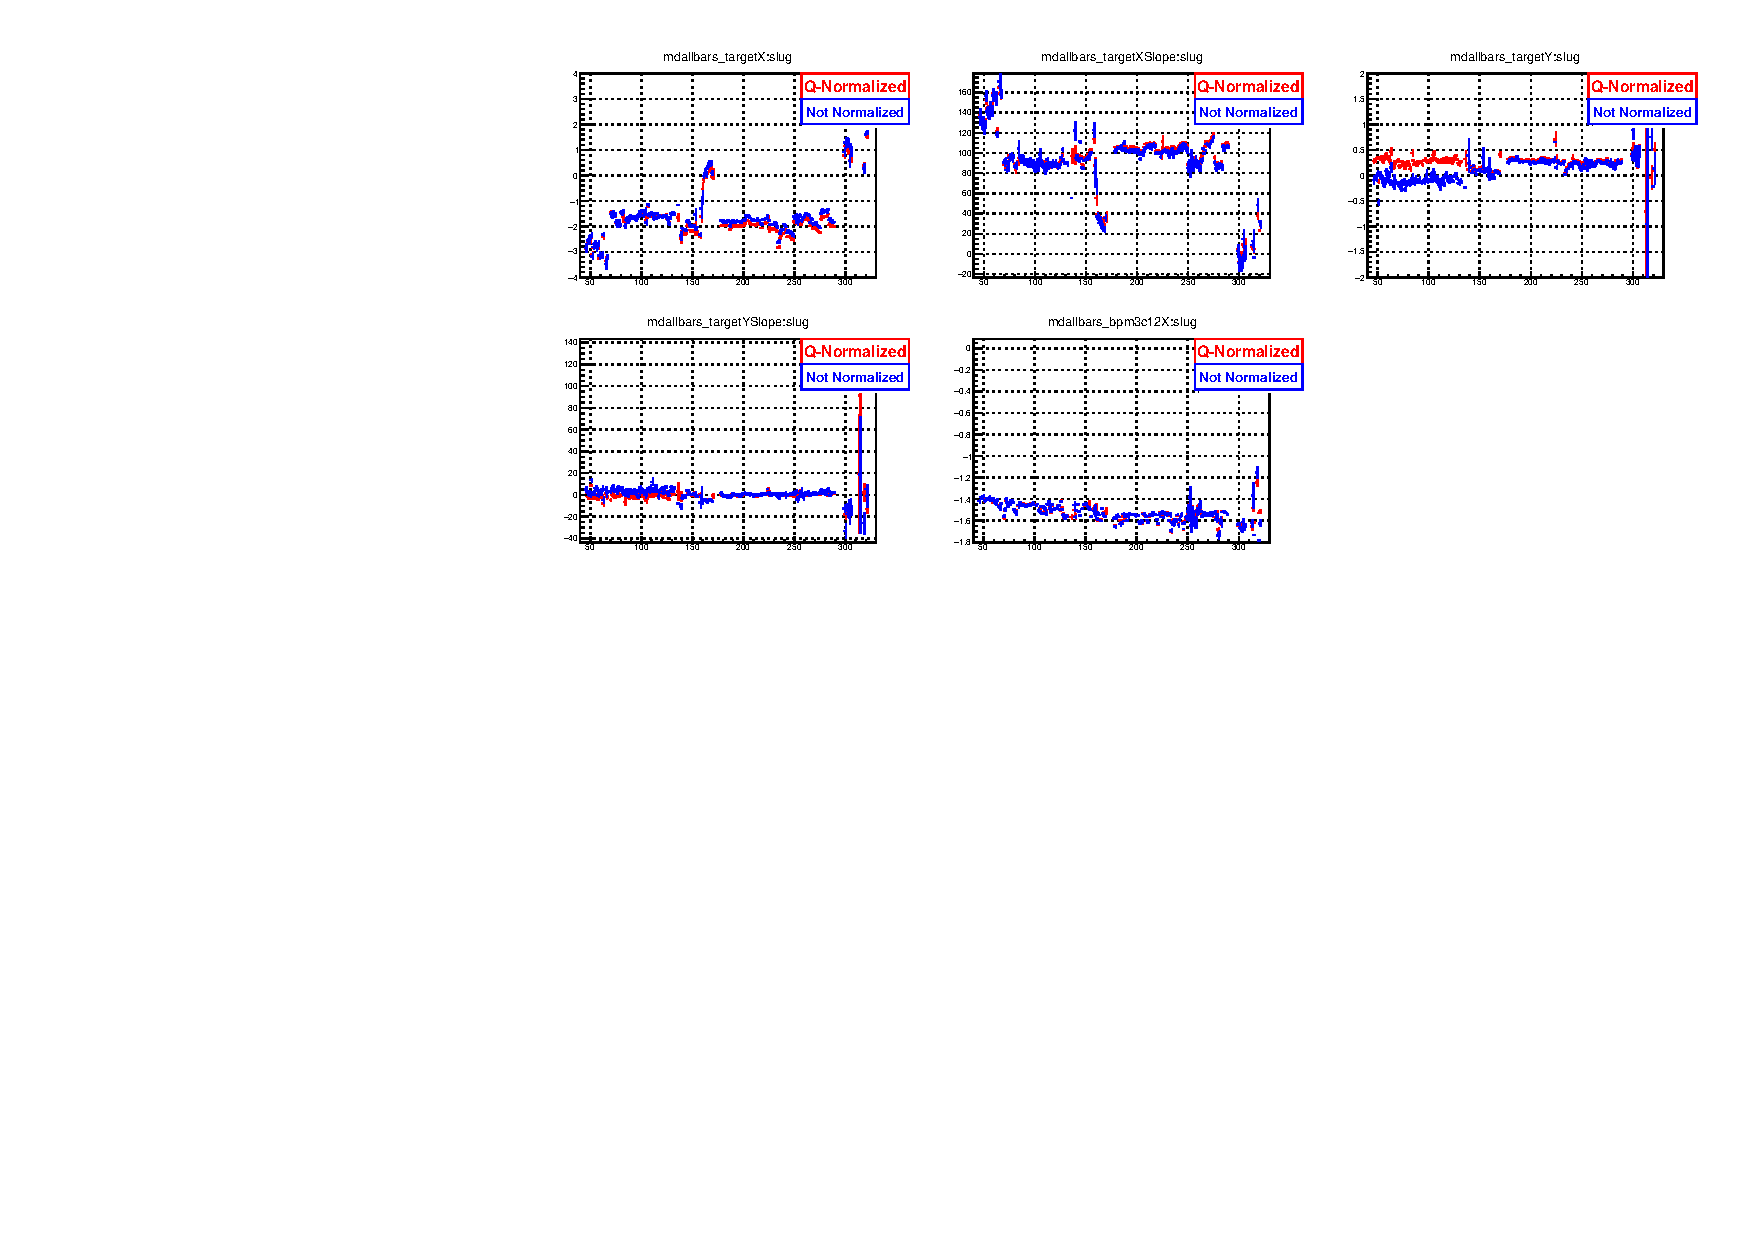
\includegraphics[width=9in]{./Pictures/NoQnorm_slopes.pdf}
\caption{\label{fig:no_Q_norm_slopes}Comparison of MDallbars correction slopes using a charge-normalized main detector and an unnormalized main detector signal. Both show equal residual sensitivities.}
\end{center}
\end{figure}


\begin{figure}[!ht]
\begin{center}
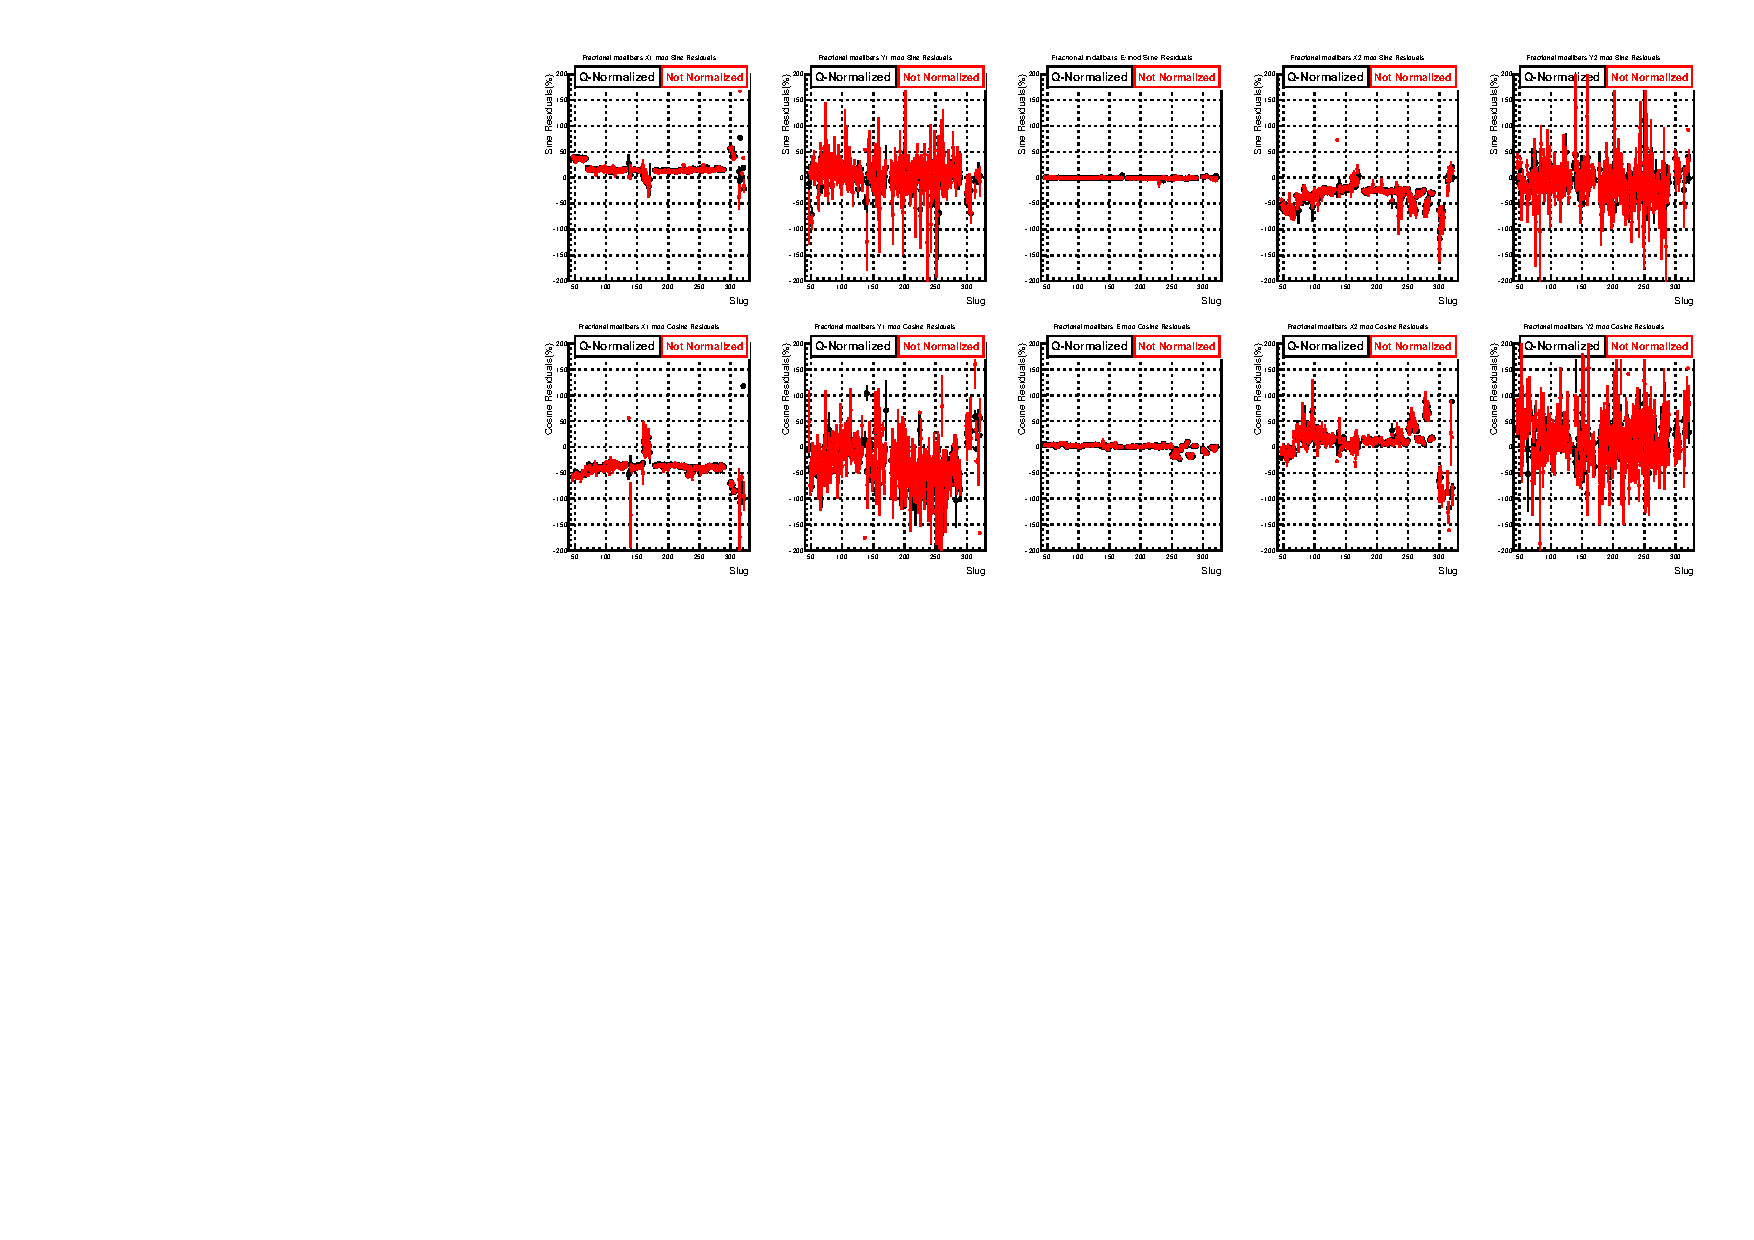
\includegraphics[width=8.9in]{./Pictures/NoQnorm_residuals.pdf}
\caption{\label{fig:no_Q_norm_residuals}Comparison of residual responses of MDallbars to modulation coils after correction using a charge-normalized main detector and an un-normalized main detector signal. Both show equal residual sensitivities.}
\end{center}
\end{figure}
\end{landscape}

\section{Determining a Beam Modulation Correction and Error}
Although the source of monopole residual sensitivity to coils after beam modulation correction remains undetermined, the signature of the inconsistency greatly limits the possible failure modes. Whatever is causing it must equally affect all main detector bars and be invisible to the beam monitors since they correct well with the same modulation analysis procedure. This signature points to an effect beyond the 5 degrees of freedom originally included in the simple linear beamline model. Something like an intrinsic beam spot size or halo modulation would seem like good candidates. These models are not completely unrealistic\footnote{Imagine a small quadrupole or higher order component to the dipole magnets driving the modulation or even electronics pickup of the modulation signal by a focusing quadrupole. These could easily change the beam spot size but it would be very difficult to detect.} but are difficult to prove. Since the modulation analysis is only correcting detectors using beam monitors, it is impossible to remove an effect to which the monitors are not sensitive. At this point it is important to find a way of deciding what correction to apply and what error to assign that reflects the uncertainty associated with inconsistencies in the analysis. The remainder of this section is devoted to developing a method for choosing a correction and assigning a systematic and statistical error to that correction.

In Section \ref{sctn:residual_correlations} almost two dozen beam modulation schemes using different coils selections were compared. It was determined that a few of these needed to be eliminated for creating residual correlations to beam monitors over long timescales or because they produced unreliable/unstable correction slopes. Much larger variations were observed in the subset of schemes where only X-type coils were omitted than in the subset omitting Y-like coils. Similarly, the residual correlations to modulation coils is much larger in the X-type coils. One scheme ``Omit 0,5'' stood out because it was the only scheme which simultaneously showed no evidence of residual sensitivity to X-type modulation coils used in the analysis and had no significant long-timescale residual correlations to beam monitors. However, the default ``10-Coil'' analysis also showed no evidence of significant long-timescale residual correlations to beam monitors. When various Y-coils were omitted from the ``10-Coil'' and ``Omit 0,5'' schemes there appeared to be two families of solutions more or less centered on the ``10-Coil'' and ``Omit 0,5'' results. Without further evidence favoring one or the other of these solutions the author proposes a straight average of the two. An estimate of the systematic error arising from the inconsistency in this analysis can be made using the spread of the data. The author proposes a conservative estimate provided by the difference from the average of the ``10-Coil'' and ``Omit 0,5'' corrections to the correction with the largest variation from this average. Looking back at tables \ref{tab:run1_dithering_corrections_table} and \ref{tab:run1_om05_dithering_corrections} for Run 1 shows the spread in total corrections to be  -11.8~ppb to -22.0~ppb. Similarly for Run 2, the spread from tables \ref{tab:run2_dithering_corrections_table} and \ref{tab:run2_om05_dithering_corrections} is -1.4~ppb to -2.6~ppb. Table \ref{tab:total_corrections} below summarizes the proposed corrections and systematic error.

\begin{table}[ht]
\caption{\label{tab:total_corrections}Proposed corrections using the average of the corrections prescribed by the ``10-Coil'' and ``Omit 0,5'' schemes. The systematic error comes from the maximum variation of other schemes from this average. Statistical error calculated from statistical spread of the correction slopes.}
\begin{center}
\Large
\begin{tabular}{|l||c|}\hline
~&~\\
\large Run 1&$\frac{-13.6-19.2}{2}=-16.4\pm 0.8(stat)\pm 5.6(syst)$~ppb\\
~&~\\
\large Run 2&$\frac{-1.7-2.4}{2}=-2.1\pm 0.3(stat)\pm 0.7(syst)$~ppb\\~&~\\\hline
\end{tabular}
\end{center}
\end{table}

In addition to the systematic error quoted above, an additional statistical error associated with the correction slopes must also be assigned. Correction slopes $\frac{\partial Detector}{\partial Monitor}$ were determined approximately every 10 minutes or as soon as sufficient information was collected to determine all the monitor and detector sensitivities to the modulation coils. One type of modulation was active for four seconds of each minute with an attempt made to cycle through all the modulation types successively. Each time a completely independent set of coil sensitivities was collected a new set of correction slopes was calculated. These short-timescale slopes were then averaged over slugs (HWP states lasting about 8~hours) and a statistical error calculated from the standard deviation divided by the square root of the number of slopes in the slug. 

The modulation correction is given by $C=\sum_j\sum_{i=1}^5w_j\left(\frac{\partial D}{\partial X_{ij}}\right)\Delta X_{ij}$ where $C$ is the correction $\frac{\partial D}{\partial X_i}$ is the correction slope of the detector to the $i$'th monitor in the $j$'th slug and $\Delta X_{ij}$ is the average of the $i$'th monitor differences over $j$'th slug. The $w_j's$ are weights applied to the corrections by slug and are the same as the main detector error weights used for calculating the average main detector asymmetry. These weights are the inverse variance of the corrected main detector asymmetry distributions divided by the number of quartet measurements in the slug ($\frac{1}{\sigma_{MD}^2/N}$). 

Using standard propagation of errors along with the main detector asymmetry error weights assigned to the main data set for each slug, allows one to calculate an estimate for the statistical error arising from the slopes. Although usual propagation of errors would involve two terms one with the error in slope times the monitor difference plus one with the error in the monitor times the slope only the former of these needs to be calculated since the latter is already included in error associated with the main detector statistical width. Propagation of errors for the first term gives
\begin{equation}
\label{eq:stat_error_cor}
\sigma_C^2=\frac{\sum_jw_j^2\sum_i\left(\delta_{ij}^{(s)} \Delta X_{ij}\right)^2}{\left(\sum_jw_j\right)^2},
\end{equation}
where $\delta_i^{(s)}$ are the statistical errors in the detector to monitor slopes at the slug level. Equation \ref{eq:stat_error_cor} assumes that the correction slopes are uncorrelated. This is clearly not the case for the monitor set used in this analysis. Slopes to targetX and targetXSlope as well as targetY and targetYSlope are highly correlated. For the purposes of estimating this error, linear combinations of these monitors were used which produced slopes that were much less correlated. Table \ref{tab:uncorrelated_monitors} shows the linear combinations used. Using slopes and statistical errors from these uncorrelated monitors gives a statistical error of 0.8~ppb for the Run 1 correction and 0.3~ppb for the Run 2 correction. These statistical errors are taken from the ``Omit 0,5'' scheme which has a larger statistical spread in its slopes. Details of a more sophisticated analysis with completely uncorrelated variables will be provided in a future thesis showing these statistical errors to be conservative \cite{Peng}.

\begin{table}[h]\
\caption{\label{tab:uncorrelated_monitors} Linear combinations of monitors used to produce semi-uncorrelated correction slopes. Units of $\mu$m for targetX(Y) and $\mu$rad for targetXSlope(YSlope) are assumed.}
\begin{center}
\begin{tabular}{l|c|c}
~&Monitor Name&Linear Combination\\\hline
Run 1 & MX1 & targetX$+35\times$targetXSlope\\
~     & MX2 & targetX$-35\times$targetXSlope\\
~     & MY1 & targetY$+29\times$targetYSlope\\
~     & MY2 & targetY$-29\times$targetYSlope\\\hline
Run 2 & MX1 & targetX$+37\times$targetXSlope\\
~     & MX2 & targetX$-37\times$targetXSlope\\
~     & MY1 & targetY$+29\times$targetYSlope\\
~     & MY2 & targetY$-29\times$targetYSlope\\
\end{tabular}
\end{center}
\end{table}
